\PassOptionsToPackage{svgnames,dvipsnames,svgnames}{xcolor}
%% For double-blind review submission
%\documentclass[acmsmall,review]{acmart}
%%% Note: arxiv does not want line numbers (they are detected somehow, and are not allowed)
\documentclass[acmsmall]{acmart}
%\settopmatter{printfolios=false,printccs=false,printacmref=false}
\settopmatter{printccs=false,printacmref=false}
\setcopyright{none}
\renewcommand\footnotetextcopyrightpermission[1]{} % removes footnote with conference information in first column

%% For single-blind review submission
%\documentclass[acmlarge,review]{acmart}\settopmatter{printfolios=true}
%% For final camera-ready submission
%\documentclass[acmlarge]{acmart}\settopmatter{}

%% Note: Authors migrating a paper from PACMPL format to traditional
%% SIGPLAN proceedings format should change 'acmlarge' to
%% 'sigplan,10pt'.

% \bibliographystyle{ACM-Reference-Format}


%% Some recommended packages.
\usepackage{booktabs}   %% For formal tables:
                        %% http://ctan.org/pkg/booktabs
\usepackage{subcaption} %% For complex figures with subfigures/subcaptions
                        %% http://ctan.org/pkg/subcaption

%% Cyrus packages
\usepackage{microtype}
\usepackage{mdframed}
\usepackage{colortab}
\usepackage{mathpartir}
\usepackage{enumitem}
\usepackage{bbm}
\usepackage{stmaryrd}
\usepackage{mathtools}
\usepackage{leftidx}
\usepackage{todonotes}
\usepackage{xspace}
\usepackage{wrapfig}


\usepackage{listings}%
\lstloadlanguages{ML}
\lstset{tabsize=2, 
basicstyle=\footnotesize\ttfamily, 
% keywordstyle=\sffamily,
commentstyle=\itshape\ttfamily\color{gray}, 
stringstyle=\ttfamily\color{purple},
mathescape=false,escapechar=\#,
numbers=left, numberstyle=\scriptsize\color{gray}\ttfamily, language=ML, showspaces=false,showstringspaces=false,xleftmargin=15pt, 
morekeywords={string, float, int},
classoffset=0,belowskip=\smallskipamount, aboveskip=\smallskipamount,
moredelim=**[is][\color{red}]{SSTR}{ESTR}
}
\newcommand{\li}[1]{\lstinline[basicstyle=\ttfamily\fontsize{9pt}{1em}\selectfont]{#1}}
\newcommand{\lismall}[1]{\lstinline[basicstyle=\ttfamily\fontsize{9pt}{1em}\selectfont]{#1}}

%% Joshua Dunfield macros
\def\OPTIONConf{1}%
\usepackage{joshuadunfield}

%% Can remove this eventually
\usepackage{blindtext}

\usepackage{enumitem}

%%%%%%%%%%%%%%%%%%%%%%%%%%%%%%%%%%%%%%%%%%%%%%%%%%%%%%%%%%%%%%%%%%%%%%%%%%%%%
%% Matt says: Cyrus, this package `adjustbox` seems directly related
%% to the `clipbox` error; To get rid of the error, I moved it last
%% (after other usepackages) and I added the line just above it, which
%% permits it to redefine `clipbox` (apparently also defined in
%% `pstricks`, and due to latex's complete lack of namespace
%% management, these would otherwise names clash).
\let\clipbox\relax
\usepackage[export]{adjustbox}% http://ctan.org/pkg/adjustbox
%%%%%%%%%%%%%%%%%%%%%%%%%%%%%%%%%%%%%%%%%%%%%%%%%%%%%%%%%%%%%%%%%%%%%%%%%%%%%%%%%


%%%%%%%%%%%%%%%%%%%%%%%%%%%%%%%%%%%%%%%%%%%%%%%%%%%%%%%%%%%%%%%%%%%%%%%%%%%%%%%%%
%\usepackage{draftwatermark}
%\SetWatermarkText{DRAFT}
%\SetWatermarkScale{1}
%%%%%%%%%%%%%%%%%%%%%%%%%%%%%%%%%%%%%%%%%%%%%%%%%%%%%%%%%%%%%%%%%%%%%%%%%%%%%%%%%


% A macro for the name of the system being described by ``this paper''
\newcommand{\HazelnutLive}{\textsf{Hazelnut Live}\xspace}
\newcommand{\Hazelnut}{\textsf{Hazelnut}\xspace}
% The mockup, work-in-progress system.
\newcommand{\Hazel}{\textsf{Hazel}\xspace}

% \newtheorem{theorem}{Theorem}[chapter]
% \newtheorem{lemma}[theorem]{Lemma}
% \newtheorem{corollary}[theorem]{Corollary}
% \newtheorem{definition}[theorem]{Definition}
% \newtheorem{assumption}[theorem]{Assumption}
% \newtheorem{condition}[theorem]{Condition}

\newtheoremstyle{slplain}% name
  {.15\baselineskip\@plus.1\baselineskip\@minus.1\baselineskip}% Space above
  {.15\baselineskip\@plus.1\baselineskip\@minus.1\baselineskip}% Space below
  {\slshape}% Body font
  {\parindent}%Indent amount (empty = no indent, \parindent = para indent)
  {\bfseries}%  Thm head font
  {.}%       Punctuation after thm head
  { }%      Space after thm head: " " = normal interword space;
        %       \newline = linebreak
  {}%       Thm head spec
\theoremstyle{slplain}
\newtheorem{thm}{Theorem}  % Numbered with the equation counter
\numberwithin{thm}{section}
\newtheorem{defn}[thm]{Definition}
\newtheorem{lem}[thm]{Lemma}
\newtheorem{prop}[thm]{Proposition}
% \newtheorem{cor}[section]{Corollary}     
% \newtheorem{lem}[section]{Lemma}         
% \newtheorem{prop}[section]{Proposition}  

% \setlength{\abovedisplayskip}{0pt}
% \setlength{\belowdisplayskip}{0pt}
% \setlength{\abovedisplayshortskip}{0pt}
% \setlength{\belowdisplayshortskip}{0pt}



\makeatletter\if@ACM@journal\makeatother
%% Journal information (used by PACMPL format)
%% Supplied to authors by publisher for camera-ready submission
\acmJournal{PACMPL}
\acmVolume{1}
\acmNumber{1}
\acmArticle{1}
\acmYear{2018}
\acmMonth{3}
\acmDOI{10.1145/nnnnnnn.nnnnnnn}
\startPage{1}
\else\makeatother
%% Conference information (used by SIGPLAN proceedings format)
%% Supplied to authors by publisher for camera-ready submission
% \acmConference[]{ACM SIGPLAN Conference on Programming Languages}{January 01--03, 2017}{New York, NY, USA}

\acmYear{2018}
\acmISBN{978-x-xxxx-xxxx-x/YY/MM}
\acmDOI{10.1145/nnnnnnn.nnnnnnn}
\startPage{1}
\fi


%% Copyright information
%% Supplied to authors (based on authors' rights management selection;
%% see authors.acm.org) by publisher for camera-ready submission
\setcopyright{none}             %% For review submission
%\setcopyright{acmcopyright}
%\setcopyright{acmlicensed}
%\setcopyright{rightsretained}
%\copyrightyear{2017}           %% If different from \acmYear


\fancyfoot{} % suppresses the footer (also need \thispagestyle{empty} after \maketitle below)


%% Bibliography style
\bibliographystyle{ACM-Reference-Format}
%% Citation style
%% Note: author/year citations are required for papers published as an
%% issue of PACMPL.
\citestyle{acmauthoryear}   %% For author/year citations

% !TEX root = main.tex

\newcommand{\mynote}[3]{\textcolor{#3}{\textsf{{#2}}}}
\newcommand{\rkc}[1]{\mynote{rkc}{#1}{blue}}
\newcommand{\cy}[1]{\mynote{cy}{#1}{purple}}
\newcommand{\mah}[1]{\mynote{cy}{#1}{green}}

\newcommand{\cvert}{{\,{\vert}\,}}

%% https://tex.stackexchange.com/questions/9796/how-to-add-todo-notes
\newcommand{\rkcTodo}[1]{\todo[linecolor=blue,backgroundcolor=blue!25,bordercolor=blue]{#1}}

\newcommand{\mattTodo}[1]{\todo[linecolor=green,backgroundcolor=green!2,bordercolor=green]{\tiny\textit{#1}}}
\newcommand{\mattOmit}[1]{\colorbox{yellow}{(Matt omitted stuff here)}}

%% SPACING HACKS
\def\parahead#1{\vspace{-8pt}\paragraph{{\textbf{#1}.}}}
\def\paraheadNoDot#1{\vspace{-8pt}\paragraph{{\textbf{#1}}}}
\def\subparahead#1{\vspace{-13pt}\paragraph{}\textit{#1.}}
\def\paraheadindent#1{\vspace{-13pt}\paragraph{}\textit{#1.}}
\def\paraheadindentnodot#1{\vspace{-13pt}\paragraph{}\textit{#1}}

% \newcommand{\ie}{{\emph{i.e.}}}
% \newcommand{\eg}{{\emph{e.g.}}}
% \newcommand{\etc}{{\emph{etc.}}}
% \newcommand{\cf}{{\emph{cf.}}}
% \newcommand{\etal}{{\emph{et al.}}}

%% \newcommand{\hazel}{\ensuremath{\textsc{Hazel}}}
%% \newcommand{\sns}{\ensuremath{\textsc{Sketch-n-Sketch}}}
%% \newcommand{\deuce}{\ensuremath{\textsc{Deuce}}}
\newcommand{\hazel}{\ensuremath{\textrm{Hazel}}}
\newcommand{\sns}{\ensuremath{\textrm{Sketch-n-Sketch}}}
\newcommand{\deuce}{\ensuremath{\textrm{Deuce}}}

\newcommand{\sectionDescription}[1]{\section{#1}}
\newcommand{\subsectionDescription}[1]{\subsection{#1}}
\newcommand{\subsubsectionDescription}[1]{\subsubsection{#1}}
%% \newcommand{\subsectionDescription}[1]{\subsection*{#1}}

\newcommand{\matt}{PI Hammer}
\newcommand{\ravi}{PI Chugh}
\newcommand{\cyrus}{Postdoc Omar}
%% \newcommand{\cuStudent}{CU Boulder Student}
%% \newcommand{\ucStudent}{UChicago Student}

\newcommand{\eap}{action suggestion panel\xspace}
\newcommand{\Eap}{Action suggestion panel\xspace}

\newcommand{\trackOne}{Track~1\xspace}
\newcommand{\trackTwo}{Track~2\xspace}
\newcommand{\trackThree}{Track~3\xspace}
\newcommand{\trackFour}{Track~4\xspace}
\newcommand{\subtrackOne}[1]{{#1}.1}
\newcommand{\subtrackTwo}[1]{{#1}.2}
\newcommand{\subtrackThree}[1]{{#1}.3}
\newcommand{\subtrackFour}[1]{{#1}.4}
\newcommand{\tracks}{Tracks}

\newcommand{\trackNameOne}{A Static Semantics for Typed Holes}
%% \newcommand{\trackNameOneOne}{Static Semantics for Incomplete Programs}
%% \newcommand{\trackNameOneTwo}{Dynamic Semantics for Incomplete Programs}

\newcommand{\trackNameTwo}{Live Programming with Typed Holes}

\newcommand{\trackNameThree}{Editing with Typed Holes}

\newcommand{\trackNameFour}{Direct Manipulation Programming with Typed Holes}
%% \newcommand{\trackNameFourOne}{Typed Projections}
%% \newcommand{\trackNameFourTwo}{Live Typed Projections}

%% \newcommand{\trackNameTwo}{Semantic Foundations for Transforming Incomplete Programs}
%% \newcommand{\trackNameTwoOne}{Edit Action Semantics}
%% \newcommand{\trackNameTwoTwo}{Structured Program Transformations} 

%% \newcommand{\trackNameThree}{Practical Applications of Interactive Structured Editing}
%% \newcommand{\trackNameThreeOne}{\hazel{}: A Hybrid Text and Structure Editor}
%% \newcommand{\trackNameThreeTwo}{Structured Editing in the Classroom}

\newcommand{\myfootnote}[1]{\footnote{ #1}}

\def\sectionautorefname{Section}
\def\subsectionautorefname{Section}
\def\subsubsectionautorefname{Section}

\newcommand{\code}[1]{\lstinline{#1}}

\newcommand{\codeSize}
  %% {\footnotesize}
  {\small}

%%%%%%%%%%%%%%%%%%%%%%%%%%%%%%%%%%%%%%%%%%%%%%%%%%%%%%%%%%%%%%%%%%%%%%%%%%%%%%%%
%% Spacing

\newcommand{\sep}{\hspace{0.06in}}
\newcommand{\sepPremise}{\hspace{0.20in}}
\newcommand{\hsepRule}{\hspace{0.20in}}
\newcommand{\vsepRuleHeight}{0.12in}
\newcommand{\vsepRule}{\vspace{\vsepRuleHeight}}
\newcommand{\miniSepOne}{\hspace{0.01in}}
\newcommand{\miniSepTwo}{\hspace{0.02in}}
\newcommand{\miniSepThree}{\hspace{0.03in}}
\newcommand{\miniSepFour}{\hspace{0.04in}}
\newcommand{\miniSepFive}{\hspace{0.05in}}

%%%%%%%%%%%%%%%%%%%%%%%%%%%%%%%%%%%%%%%%%%%%%%%%%%%%%%%%%%%%%%%%%%%%%%%%%%%%%%%%

% \lstset{
% %mathescape=true,basicstyle=\fontsize{8}{9}\ttfamily,
% literate={=>}{$\Rightarrow$}2
%          {<=}{$\leq$}2
%          {->}{${\rightarrow}$}1
%          {\\\\=}{\color{red}{$\lambda$}}2
%          {\\\\}{$\lambda$}2
%          {**}{$\times$}2
%          {*.}{${\color{blue}{\texttt{*.}}}$}2
%          {+.}{${\color{blue}{\texttt{+.}}}$}2
%          {<}{${\color{green}{\lhd}}$}1
%          {>?}{${\color{green}{\rhd}}$?}2
%          {<<}{${\color{green}{\blacktriangleleft}}$}1
%          {>>?}{${\color{green}{\blacktriangleright}}$?}2
%          {\{}{${\color{blue}{\{}}$}1
%          {\}}{${\color{blue}{\}}}$}1
%          {[}{${\color{purple}{[}}$}1
%          {]}{${\color{purple}{]}}$}1
%          {(}{${\color{darkgray}{\texttt{(}}}$}1
%          {)}{${\color{darkgray}{\texttt{)}}}$}1
%          {]]}{${\color{gray}{\big(}}$}1
%          {]]}{${\color{gray}{\big)}}$}1
% }

% !TEX root = hazelnut-dynamics.tex

% Violet hotdogs; highlight color helps distinguish them
\newcommand{\llparenthesiscolor}{\textcolor{violet}{\llparenthesis}}
\newcommand{\rrparenthesiscolor}{\textcolor{violet}{\rrparenthesis}}
% \newcommand{\llparenthesiscolor}{\textcolor{red}{\lfloor}}
% \newcommand{\rrparenthesiscolor}{\textcolor{red}{\rfloor}}

%% TODO if feeling really obsessive, use the following two in place of x and u
\newcommand{\varVar}{x}
\newcommand{\varHole}{u}

% HTyp and HExp
\newcommand{\hcomplete}[1]{#1~\mathsf{complete}}

% HTyp
\newcommand{\htau}{\tau}
\newcommand{\tarr}[2]{#1 \rightarrow #2}
\newcommand{\tprod}[2]{#1 \times #2}
\newcommand{\tnum}{\texttt{num}}
\newcommand{\tb}{\texttt{b}}
\newcommand{\tehole}{\llparenthesiscolor\rrparenthesiscolor}
\newcommand{\tsum}[2]{{#1} + {#2}}

\newcommand{\tconsistent}[2]{#1 \sim #2}
\newcommand{\tinconsistent}[2]{#1 \nsim #2}

% HExp
\newcommand{\hexp}{e}
\newcommand{\hlam}[2]{\lambda #1.#2}
\newcommand{\halam}[3]{\lambda #1{:}#2.#3}
\newcommand{\hap}[2]{#1(#2)}
\newcommand{\hapP}[2]{(#1)~(#2)} % Extra paren around function term
\newcommand{\hpair}[2]{(#1, #2)}
\newcommand{\hprj}[2]{\mathsf{prj}_{#1}(#2)}
\newcommand{\lblL}{\mathsf{L}}
\newcommand{\lblR}{\mathsf{R}}
\newcommand{\hnum}[1]{\underline{#1}}
\newcommand{\hadd}[2]{#1 + #2}
\newcommand{\hehole}[1]{\llparenthesiscolor\rrparenthesiscolor^{#1}}
% \newcommand{\hhole}[1]{\setlength{\fboxsep}{0pt}\fcolorbox{red}{white}{\vphantom{)}$#1$}}
\newcommand{\hhole}[2]{\llparenthesiscolor#1\rrparenthesiscolor^{#2}}
% \newcommand{\hhole}[1]{
  % \setlength{\fboxsep}{0pt}
  % \colorbox{violet!10!white!100}{\ensuremath{\llparenthesiscolor#1\rrparenthesiscolor}}}
\newcommand{\hindet}[1]{\lceil#1\rceil}
\newcommand{\hinj}[2]{\texttt{inj}_{#1}({#2})}
\newcommand{\hcase}[5]{\texttt{case}({#1},{#2}.{#3},{#4}.{#5})}

\newcommand{\hGamma}{\Gamma}
\newcommand{\domof}[1]{\text{dom}(#1)}
\newcommand{\hsyn}[3]{#1 \vdash #2 \Rightarrow #3}
\newcommand{\hana}[3]{#1 \vdash #2 \Leftarrow #3}

% ZTyp and ZExp
\newcommand{\zlsel}[1]{{\bowtie}{#1}}
\newcommand{\zrsel}[1]{{#1}{\bowtie}}

%\newcommand{\zwsel}[1]{\adjustbox{cframe=blue}{\ensuremath{{\textcolor{blue}{\triangleright}}{#1}{\textcolor{blue}{\triangleleft}}}}}
\newcommand{\zwsel}[1]{
  \setlength{\fboxsep}{0pt}
  \colorbox{green!10!white!100}{
    \ensuremath{{{\textcolor{Green}{{\hspace{-2px}\triangleright}}}}{#1}{\textcolor{Green}{\triangleleft{\vphantom{\tehole}}}}}}
}
%\newcommand{\zwsel}[1]{{\triangleright}{#1}{\triangleleft}}

\newcommand{\removeSel}[1]{#1^{\diamond}}

% ZTyp
\newcommand{\ztau}{\hat{\tau}}

% ZExp
\newcommand{\zexp}{\hat{e}}

% Direction
\newcommand{\dParent}{\mathtt{parent}}
\newcommand{\dChild}{\mathtt{firstChild}}
\newcommand{\dNext}{\mathtt{nextSib}}
\newcommand{\dPrev}{\mathtt{prevSib}}

% Action
\newcommand{\aMove}[1]{\mathtt{move}~#1}
	\newcommand{\zrightmost}[1]{\mathsf{rightmost}(#1)}
	\newcommand{\zleftmost}[1]{\mathsf{leftmost}(#1)}
\newcommand{\aSelect}[1]{\mathtt{sel}~#1}
\newcommand{\aDel}{\mathtt{del}}
\newcommand{\aReplace}[1]{\mathtt{replace}~#1}
\newcommand{\aConstruct}[1]{\mathtt{construct}~#1}
\newcommand{\aConstructx}[1]{#1}
\newcommand{\aFinish}{\mathtt{finish}}

\newcommand{\performAna}[5]{#1 \vdash #2 \xlongrightarrow{#4} #5 \Leftarrow #3}
\newcommand{\performAnaI}[5]{#1 \vdash #2 \xlongrightarrow{#4}\hspace{-3px}{}^{*}~ #5 \Leftarrow #3}
\newcommand{\performSyn}[6]{#1 \vdash #2 \Rightarrow #3 \xlongrightarrow{#4} #5 \Rightarrow #6}
\newcommand{\performSynI}[6]{#1 \vdash #2 \Rightarrow #3 \xlongrightarrow{#4}\hspace{-3px}{}^{*}~ #5 \Rightarrow #6}
\newcommand{\performTyp}[3]{#1 \xlongrightarrow{#2} #3}
\newcommand{\performTypI}[3]{#1 \xlongrightarrow{#2}\hspace{-3px}{}^{*}~#3}

\newcommand{\performMove}[3]{#1 \xlongrightarrow{#2} #3}
\newcommand{\performDel}[2]{#1 \xlongrightarrow{\aDel} #2}

% Form
\newcommand{\farr}{\mathtt{arrow}}
\newcommand{\fnum}{\mathtt{num}}
\newcommand{\fsum}{\mathtt{sum}}

\newcommand{\fasc}{\mathtt{asc}}
\newcommand{\fvar}[1]{\mathtt{var}~#1}
\newcommand{\flam}[1]{\mathtt{lam}~#1}
\newcommand{\fap}{\mathtt{ap}}
\newcommand{\farg}{\mathtt{arg}}
\newcommand{\fnumlit}[1]{\mathtt{lit}~#1}
\newcommand{\fplus}{\mathtt{plus}}
\newcommand{\fhole}{\mathtt{hole}}
\newcommand{\fnehole}{\mathtt{nehole}}

\newcommand{\finj}[1]{\mathtt{inj}~#1}
\newcommand{\fcase}[2]{\mathtt{case}~#1~#2}

% Talk about formal rules in example
\newcommand{\refrule}[1]{\textrm{Rule~(#1)}}

\newcommand{\herase}[1]{\left|#1\right|_\textsf{erase}}

\newcommand{\arrmatch}[2]{#1 \blacktriangleright_{\rightarrow} #2}
\newcommand{\prodmatch}[2]{#1 \blacktriangleright_{\times} #2}
\newcommand{\summatch}[2]{#1 \blacktriangleright_{+} #2}


\newcommand{\TABperformAna}[5]{#1 \vdash & #2                & \xlongrightarrow{#4} & #5 & \Leftarrow #3}
\newcommand{\TABperformSyn}[6]{#1 \vdash & #2 \Rightarrow #3 & \xlongrightarrow{#4} & #5 \Rightarrow #6}
\newcommand{\TABperformTyp}[3]{& #1 & \xlongrightarrow{#2} & #3}

\newcommand{\TABperformMove}[3]{#1 & \xlongrightarrow{#2} & #3}
\newcommand{\TABperformDel}[2]{#1 \xlongrightarrow{\aDel} #2}

\newcommand{\sumhasmatched}[2]{#1 \mathrel{\textcolor{black}{\blacktriangleright_{+}}} #2}

%%%% DYNAMICS %%%%
%% TODO remove these macros
%% marks for eval
\newcommand{\unevaled}{\times}
\newcommand{\evaled}{\checkmark}
\newcommand{\markname}{m}

\newcommand{\mvar}[0]{u}
\newcommand{\subst}[0]{\sigma}
\newcommand{\dexp}[0]{d}
\newcommand{\dconst}[0]{c}
\newcommand{\dval}[0]{\ddot{v}}
%% TODO remove this macro
\newcommand{\dcast}[2]{\langle #1 \rangle ~ #2}
%% TODO make the following two look better
\newcommand{\dcasttwo}[3]{#1 \langle{#2}\Rightarrow{#3}\rangle}
\newcommand{\dcastthree}[4]{#1 \langle{#2}\Rightarrow{#3}\Rightarrow{#4}\rangle}
\newcommand{\dcastfail}[4]{#1 \langle{#2}\Rightarrow{#3}\not\Rightarrow{#4}\rangle}
\newcommand{\dlam}[3]{\lambda #1:#2.#3}
\newcommand{\dap}[2]{#1(#2)}
\newcommand{\dapP}[2]{(#1)(#2)} % Extra paren around function term
\newcommand{\dnum}[1]{\underline{#1}}
\newcommand{\dadd}[2]{#1 + #2}
\newcommand{\dehole}[3]{\leftidx{^{#3}}{\llparenthesiscolor\rrparenthesiscolor}{^{#1}_{#2}}}
\newcommand{\dhole}[4]{\leftidx{^{#4}}{\llparenthesiscolor#1\rrparenthesiscolor}{^{#2}_{#3}}}
\newcommand{\dindet}[1]{\lceil#1\rceil}
\newcommand{\dinj}[2]{\texttt{inj}_{#1}({#2})}
\newcommand{\dcase}[5]{\texttt{case}({#1},{#2}.{#3},{#4}.{#5})}

\newcommand{\expandAna}[6]{#1 \vdash #2 \Leftarrow #3 \leadsto #4 : #5 \dashv #6}
\newcommand{\expandSyn}[5]{#1 \vdash #2 \Rightarrow #3 \leadsto #4 \dashv #5}
\newcommand{\hasType}[4]{#1; #2 \vdash #3 : #4}
\newcommand{\isValue}[1]{#1~\mathsf{val}}
\newcommand{\isIndet}[1]{#1~\mathsf{indet}}
\newcommand{\isFinal}[1]{#1~\mathsf{final}}
\newcommand{\isErr}[2]{#1 \vdash #2~\mathsf{err}}
%% \newcommand{\stepsTo}[2]{#1 \mapsto_{\Delta} #2}
\newcommand{\stepsToD}[3]{#1 \vdash #2 \mapsto #3}

%% TODO if feeling obsessive, replace direct uses of \Delta
\newcommand{\hDelta}{\Delta}
\newcommand{\Dunion}[2]{#1 \cup #2}
\newcommand{\idof}[1]{\mathsf{id}(#1)}
\newcommand{\Dbinding}[3]{#1 :: [#2]#3}

% Contextual dynamics
\newcommand{\evalctx}{\mathcal{E}}
\newcommand{\evalhole}{\circ}
\newcommand{\isevalctx}[1]{#1~\mathsf{evalCtx}}
\newcommand{\reducesE}[3]{#1 \vdash #2 \longrightarrow #3}
\newcommand{\selectEvalCtxR}[2]{#1\{#2\}}
\newcommand{\selectEvalCtx}[3]{#1=\selectEvalCtxR{#2}{#3}}


\setlength{\abovecaptionskip}{4pt plus 3pt minus 2pt} % Chosen fairly arbitrarily
\setlength{\belowcaptionskip}{-4pt plus 3pt minus 2pt} % Chosen fairly arbitrarily


\begin{document}

%% Title information
\title{Live Functional Programming with Typed Holes}         %% [Short Title] is optional;
                                        %% when present, will be used in
                                        %% header instead of Full Title.
% \titlenote{with title note}             %% \titlenote is optional;
                                        %% can be repeated if necessary;
                                        %% contents suppressed with 'anonymous'
% \subtitle{Subtitle}                     %% \subtitle is optional
% \subtitlenote{with subtitle note}       %% \subtitlenote is optional;
                                        %% can be repeated if necessary;
                                        %% contents suppressed with 'anonymous'


%% Author information
%% Contents and number of authors suppressed with 'anonymous'.
%% Each author should be introduced by \author, followed by
%% \authornote (optional), \orcid (optional), \affiliation, and
%% \email.
%% An author may have multiple affiliations and/or emails; repeat the
%% appropriate command.
%% Many elements are not rendered, but should be provided for metadata
%% extraction tools.

%% Author with single affiliation.
\author{Cyrus Omar}
% \authornote{with author1 note}          %% \authornote is optional;
                                        %% can be repeated if necessary
% \orcid{nnnn-nnnn-nnnn-nnnn}             %% \orcid is optional
\affiliation{
  % \position{Position1}
  % \department{Department1}              %% \department is recommended
  \institution{University of Chicago}            %% \institution is required
  % \streetaddress{Street1 Address1}
  % \city{City1}
  % \state{State1}
  % \postcode{Post-Code1}
  % \country{Country1}
}
\email{comar@cs.uchicago.edu}          %% \email is recommended

\author{Ian Voysey}
% \authornote{with author1 note}          %% \authornote is optional;
                                        %% can be repeated if necessary
% \orcid{nnnn-nnnn-nnnn-nnnn}             %% \orcid is optional
\affiliation{
  % \position{Position1}
  % \department{Department1}              %% \department is recommended
  \institution{Carnegie Mellon University}            %% \institution is required
  % \streetaddress{Street1 Address1}
  % \city{City1}
  % \state{State1}
  % \postcode{Post-Code1}
  % \country{Country1}
}
\email{iev@cs.cmu.edu}          %% \email is recommended

\author{Ravi Chugh}
% \authornote{with author1 note}          %% \authornote is optional;
                                        %% can be repeated if necessary
% \orcid{nnnn-nnnn-nnnn-nnnn}             %% \orcid is optional
\affiliation{
  % \position{Position1}
  % \department{Department1}              %% \department is recommended
  \institution{University of Chicago}            %% \institution is required
  % \streetaddress{Street1 Address1}
  % \city{City1}
  % \state{State1}
  % \postcode{Post-Code1}
  % \country{Country1}
}
\email{rchugh@cs.uchicago.edu}          %% \email is recommended

\author{Matthew A. Hammer}
% \authornote{with author1 note}          %% \authornote is optional;
                                        %% can be repeated if necessary
% \orcid{nnnn-nnnn-nnnn-nnnn}             %% \orcid is optional
\affiliation{
  % \position{Position1}
  % \department{Department1}              %% \department is recommended
  \institution{University of Colorado Boulder}            %% \institution is required
  % \streetaddress{Street1 Address1}
  % \city{City1}
  % \state{State1}
  % \postcode{Post-Code1}
  % \country{Country1}
}
\email{matthew.hammer@colorado.edu}          %% \email is recommended


% %% Author with two affiliations and emails.
% \author{First2 Last2}
% \authornote{with author2 note}          %% \authornote is optional;
%                                         %% can be repeated if necessary
% \orcid{nnnn-nnnn-nnnn-nnnn}             %% \orcid is optional
% \affiliation{
%   \position{Position2a}
%   \department{Department2a}             %% \department is recommended
%   \institution{Institution2a}           %% \institution is required
%   \streetaddress{Street2a Address2a}
%   \city{City2a}
%   \state{State2a}
%   \postcode{Post-Code2a}
%   \country{Country2a}
% }
% \email{first2.last2@inst2a.com}         %% \email is recommended
% \affiliation{
%   \position{Position2b}
%   \department{Department2b}             %% \department is recommended
%   \institution{Institution2b}           %% \institution is required
%   \streetaddress{Street3b Address2b}
%   \city{City2b}
%   \state{State2b}
%   \postcode{Post-Code2b}
%   \country{Country2b}
% }
% \email{first2.last2@inst2b.org}         %% \email is recommended


%% Paper note
%% The \thanks command may be used to create a "paper note" ---
%% similar to a title note or an author note, but not explicitly
%% associated with a particular element.  It will appear immediately
%% above the permission/copyright statement.
% \thanks{with paper note}                %% \thanks is optional
                                        %% can be repeated if necesary
                                        %% contents suppressed with 'anonymous'


%% Abstract
%% Note: \begin{abstract}...\end{abstract} environment must come
%% before \maketitle command
% !TEX root = hazelnut-dynamics.tex

\begin{abstract}

  
%%%%%%%%%%%%%%%%%%%%%%%%%%%%%%%%%%%%%%%%%%%%%%%%%%%%%%%%%%%%%%%%%%%%%%%%%%%%%%%%%%%%%%%%%%%%%%
%% PAR 1: Live programming environments --- Problem statement
%%%%%%%%%%%%%%%%%%%%%%%%%%%%%%%%%%%%%%%%%%%%%%%%%%%%%%%%%%%%%%%%%%%%%%%%%%%%%%%%%%%%%%%%%%%%%%
  
Live programming environments aim to provide programmers (and sometimes audiences) 
with continuous feedback about a program's dynamic behavior as it is being edited. 
%
The problem is that programming languages typically assign dynamic meaning only 
 to programs that are \emph{complete}, i.e. syntactically well-formed and free
of type errors. Consequently,    
live feedback presented to the programmer exhibits temporal or perceptive gaps, i.e. it flickers out or it goes stale whenever the program becomes incomplete. 
% In some cases, these gaps persist over a substantial length of time.
%
% Defining a semantics for incomplete functional programs would help bridge the
% gap between well-formed states and allow live programming environments to
% provide continuous, uninterrupted, and meaningful feedback.

%%%%%%%%%%%%%%%%%%%%%%%%%%%%%%%%%%%%%%%%%%%%%%%%%%%%%%%%%%%%%%%%%%%%%%%%%%%%%%%%%%%%%%%%%%%%%%
%% PAR 2: This paper's approach: New (dynamic) semantics for incomplete programs
%%%%%%%%%%%%%%%%%%%%%%%%%%%%%%%%%%%%%%%%%%%%%%%%%%%%%%%%%%%%%%%%%%%%%%%%%%%%%%%%%%%%%%%%%%%%%%

This paper confronts this ``{gap problem}'' from type-theoretic first principles by developing 
\emph{a dynamic semantics for incomplete functional programs}, 
starting from the static semantics of \citet{popl-paper}. 
%
We model incomplete functional programs as expressions with \emph{holes}, 
with empty holes standing for missing expressions or types, and  non-empty holes 
operating as membranes around static and dynamic type inconsistencies. 
%
Rather than aborting when evaluation encounters any of these holes as in
some existing systems, evaluation proceeds around holes,
tracking the 
closure around each hole instance as it flows through the remainder of the program. Editor services can use the information in these hole closures 
to help the programmer develop and confirm their mental model of the behavior of the complete portions of the program as they decide how to fill the remaining holes. 
Hole closures also enable a \emph{fill-and-resume} operation that 
avoids the need to restart evaluation after edits that amount to hole filling. 
Formally, the semantics borrows machinery from both gradual type theory (to handle unfillable 
type holes) and contextual modal type theory (which supplies the
logical basis for hole closures), combining these and developing additional machinery necessary 
to continue evaluation past holes while maintaining type safety. We have mechanized the metatheory of the core calculus, called \HazelnutLive{}, using the Agda proof assistant.

%%%%%%%%%%%%%%%%%%%%%%%%%%%%%%%%%%%%%%%%%%%%%%%%%%%%%%%%%%%%%%%%%%%%%%%%%%%%%%%%%%%%%%%%%%%%%%
%% PAR 3: We have an implementation, and have proofs
%%%%%%%%%%%%%%%%%%%%%%%%%%%%%%%%%%%%%%%%%%%%%%%%%%%%%%%%%%%%%%%%%%%%%%%%%%%%%%%%%%%%%%%%%%%%%%

% , including 
% (1) a type safety property that accounts for expression holes (i.e. free metavariables, 
% from the perspective of CMTT) and cast failure holes (which provide a novel), and (2) a commutativity property that establishes that the
% ``edit-and-resume'' feature is sound.
%
%
We have also implemented these ideas into the \Hazel programming environment. The implementation inserts holes automatically, following the \Hazelnut edit action calculus of \citet{popl-paper}, to guarantee that every editor state has some (possibly incomplete)
type.
Taken together with this paper's type safety property, the 
% The 
result is  
a proof-of-concept live programming environment where rich dynamic feedback 
is truly available without gaps, i.e. for every reachable editor state.
% i.e. \emph{every edit state is guaranteed to have
% non-trivial static and dynamic meaning}.

%In our system, evaluation treats failed casts much like it treats expression holes (rather than immediately failing with a cast error, as in gradual type theory). Prior work on contextual modal type theory did not develop an operational semantics for programs with free metavariables, which correspond to programs with holes in our formulation. 


% These incomplete edit states are sometimes transient, but at other times, they persist for extended periods of time, e.g. when the programmer is filling in the branches of a large case analysis one-by-one, or when an edit causes type errors to appear throughout a program. %This gap can cause live programming services to lag behind the programmer's edits, in many cases for an extended period of time.
\end{abstract}



%% 2012 ACM Computing Classification System (CSS) concepts
%% Generate at 'http://dl.acm.org/ccs/ccs.cfm'.
% \begin{CCSXML}
% <ccs2012>
% <concept>
% <concept_id>10011007.10011006.10011008</concept_id>
% <concept_desc>Software and its engineering~General programming languages</concept_desc>
% <concept_significance>500</concept_significance>
% </concept>
% <concept>
% <concept_id>10003456.10003457.10003521.10003525</concept_id>
% <concept_desc>Social and professional topics~History of programming languages</concept_desc>
% <concept_significance>300</concept_significance>
% </concept>
% </ccs2012>
% \end{CCSXML}

% \ccsdesc[500]{Software and its engineering~General programming languages}
% \ccsdesc[300]{Social and professional topics~History of programming languages}
%% End of generated code


%% Keywords
%% comma separated list
% \keywords{keyword1, keyword2, keyword3}  %% \keywords is optional


%% \maketitle
%% Note: \maketitle command must come after title commands, author
%% commands, abstract environment, Computing Classification System
%% environment and commands, and keywords command.
\maketitle
\thispagestyle{empty} % suppresses the footer

% !TEX root = hazelnut-popl17.tex

%% There are some benefits to this approach, to be sure, but the structural
%% mismatch between programs and their textual representations also imposes
%% various burdens.  For example, the primitive edit actions available in a
%% text editor (e.g. inserting or deleting a character or word) do not
%% always correspond to sensible structural transformations.

% spj: describe the problem; state our contributions; STOP. one page max.

% When constructing a program or proof in a language with rich type
% structure, skilled programmers generally follow a \emph{type discipline}
% where they first determine the type of the expression that they are
% constructing in order to constrain the mental search space that they are
% operating within.

% For example, if the programmer knows that an expression of type
% $\tarr{\tnum}{\tnum}$ is needed, then it is often the case (though, of course, not
% necessarily the case) that the expression will take the form $$\hlam{\mathit{x}}{e}$$
% for some variable $x$ and function body $e$. If the programmer chooses this
% form, then after picking a suitable variable name, her focus will be on
% constructing a suitable body, $e$. Following the type discipline, $e$ must
% be of type $\tnum$, and so this process can begin anew.

% The problem is that when using a text
% editor to construct a program, it is easy, and indeed necessary, to deviate from this disciplined process.  Rather, text editors operate on sequences of
% characters (i.e. \emph{text}.) 

%Although programs can be represented as text, most text does not correspond to a syntactically well-formed and semantically well-defined program. 
% Programming languages, and therefore programs themselves, are rich mathematical structures.
Programmers typically construct and manipulate well-typed expressions only indirectly, by editing text that is first parsed according to a textual syntax and then typechecked according to a static semantics. This indirection has practical benefits, to be sure -- text editors and other text-based tools benefit from decades of development effort -- but it also introduces some fundamental complexity into the programming process. 

% Every day, programmers use text-based tools to construct and manipulate programs.  
% These programs are written in languages which defined by a textual syntax. 
% While textual syntax has proved to have practical utility, it also introduces some fundamental complexity into the programming process.

% It also complicates matters for tool designers because tools are often confronted with text that does not correspond to a well-formed, meaningful program\todo{mention YoungSeok's data here}. This may be because the programmer is in the midst of a sequence of 
% edit actions that leaves the text temporarily malformed or ill-typed, or because the programmer has made a mistake. The language definition is silent about these situations, so it is difficult for tools to help programmers determine and execute a corrective course of action (e.g. by providing \todo{cite study on benefits of syntax highlighting}syntax highlighting and semantics-aware code completion services\todo{cite something?}.)
%Doesn't really start out with a bang, IMHO. I like to start papers out with a "big" problem.
%Most programming languages define a textual syntax. This allows programmers to use text editors and other standard text-based tools to construct and manipulate programs. While this is of substantial practical utility, it also introduces some fundamental complexity into the programming process. 

First, it requires that programmers learn the subtleties of the textual syntax (e.g. the precedence of the various forms.) This can be particularly challenging for novices \cite{Altadmri:2015:MCI:2676723.2677258}. %For example, one study of novice programmers found syntax errors (e.g. unbalanced parentheses) to be the most common class of errors.
% Too much detail? 

The fact that not every sequence of characters corresponds to a meaningful program also complicates matters for tool designers. In particular, program editors must contend with meaningless text on a regular basis. In a dataset analyzed by Yoon and Myers consisting of 1460 hours of edit logs, 44.2\% of edit states were syntactically malformed \cite{6883030}. Some additional percentage of edit states were well-formed but ill-typed (the dataset did not contain enough information to determine the exact percentage.)  
Some of these meaningless edit states arose because the programmer was in the midst of a sequence of edits that left the edit state transiently meaningless, while others arose because the programmer made a logical mistake. Because the language definitions is silent about these edit states, it is difficult to design useful editor services, e.g. syntax highlighting~\cite{sarkar2015impact}, type-aware code completion~\cite{Mooty:2010:CCC:1915084.1916348,Omar:2012:ACC:2337223.2337324}, and refactoring support \cite{mens2004survey}. Editors must either disable these editor services when they encounter meaningless edit states or develop \emph{ad hoc} heuristics, which can be misleading. %, or because the programmer has made a mistake. 
% The syntax definition is silent about these situations, so it is difficult for tools to help programmers determine and execute a corrective course of action 

% Many editors have developed \emph{ad hoc} workarounds for this problem, e.g. they might attempt to use regular expressions to highlight malformed program text, insert closing delimiters automatically, use whitespace to guess where a delimiter is likely to appear, or continue past a type error by pretending that the type was as expected (if, indeed, an expected type can be determined.) These heuristic methods are often complex, and they can confuse or mislead the programmer. % This may also help explain why the error messages emitted by parsers and typecheckers are often quite baroque\todo{citations}.

% stuck editing a representation of the program instead of the structures
% themselves. The editor does not restrict what the programmer may do: you
% can delete characters that belong, insert ones that don't, forget things
% that were needed, and so. There's nothing stopping us from accidentally
% writing $$\lambda \mathit{x:num}.\mathit{(x,x)}$$ even though it's obvious
% that building a pair can't hope to form a natural number.

% The type structure of the language makes this sort of error obvious: it's
% not that you're adding characters that make your program incorrect, or even
% malformed; you're adding characters that can't possibly create a structure
% you want because of the type. Simply put, the primitive operations
% available in text editors do not always correspond to sensible
% transformations on the structure of the program.
These complications have motivated a long line of research into \emph{structure editors}, i.e. program editors where every edit state is a program structure. % Eliminating text eliminates the possibility of syntax errors.

Most structure editors are \emph{syntactic structure editors}, i.e. the edit state is a syntax tree with \emph{holes} that stand for branches of the tree that have yet to be constructed, and the edit actions are context-free tree transformations. For example, Scratch is a syntactic structure editor that has achieved success as a tool for teaching children how to program \cite{Resnick:2009:SP:1592761.1592779}. 

The Scratch language has a trivial static semantics, but researchers have also designed syntactic structure editors for  languages with a non-trivial static semantics. For example, \texttt{mbeddr} is an editor for a C-like language \cite{voelter_mbeddr:_2012}, TouchDevelop is an editor for an object-oriented language \cite{tillmann_touchdevelop:_2011} and Lamdu is an editor for a functional language similar to Haskell \cite{lamdu}. Each of these editors presents an innovative user interface, but the non-trivial type and binding structure of the underlying language complicates its design. The reason is that a syntactic structure editor does not guarantee that every edit state is statically meaningful -- only that it is syntactically well-formed. As in textual program editors, these syntactic structure editors must either disable key editor services when they encounter meaningless edit states or deploy \emph{ad hoc} heuristics.
%Indeed, it is not entirely clear what it should mean for terms with holes to be statically meaningful. 
% Consequently, heuristics analagous to those that pervade textual program editors also pervade these syntactic structure editors.

% \begin{itemize}
% \item 

% First, there is an all too familiar problem: these languages do not have a clear formal semantics and metatheory, i.e. ``the implementation is the specification''. This makes it difficult to reason methodically about types and binding, so, in turn, it is difficult to design reliable editor services.

% Even if a formal semantics and metatheory for the underlying language were forthcoming (e.g. following Standard ML \cite{Harper00atype-theoretic,mthm97-for-dart}), it would go only part of the way towards addressing the challenges faced by structure editor designers. First, a standard semantics assigns no formal meaning to \emph{incomplete terms}, i.e. terms with holes. Moreover, a syntactic structure editor  -- so incorporating holes into the static semantics would in any case be only a minor salve. Heuristics analagous to those that pervade textual program editors would still be needed to contend with the ill-typed edit states.

This paper develops a principled solution to this problem. We introduce Hazelnut,  a \emph{typed structure editor}  based on a bidirectionally typed lambda calculus extended to assign static meaning to expressions and types with {holes}, which we call \textbf{H-expressions} and \textbf{H-types}. Hazelnut's formal \emph{action semantics} maintains the invariant that every edit state is a statically meaningful (i.e. well-typed) H-expression with a single superimposed \emph{cursor}. We call H-expressions and H-types with a cursor \textbf{Z-expressions} and \textbf{Z-types} (so prefixed because our encoding follows Huet's \emph{zipper} pattern \cite{JFP::Huet1997}.) %ctions act relative to the H-expression or H-type under the cursor.% (which need not be a hole.)  %More specifically, actions are context-aware,  acting on an expression whose type is determined by its surroundings (e.g. a function argument), only actions consistent with that type are permitted. 

Na\"ively, enforcing an injunction on ill-typed edit states would force programmers to construct programs in a rigid ``outside-in'' manner. For example, the programmer would often need to construct the outer function application form before identifying the intended function. To address this problem, Hazelnut leaves newly constructed expressions \emph{inside} a hole if the expression's type is inconsistent with the expected type. This meaningfully defers the type consistency check until the expression inside the hole is \emph{finished}. In other words, holes appear both at the leaves and at the internal nodes of an H-expression that remain under construction. %In short, Hazelnut is a \emph{bidirectionally typed structure editor calculus}. %Actions act at a programmer-indicate subtree, called the \emph{focus} (which is defined following Huet's zipper pattern.) 

% By defining \emph{holes} as a language construct, for both expressions as types, Hazelnut enables type-aware actions that always leave the program in both a structurally and semantically well-defined state. 
%In Hazelnut, expressions and types with \emph{holes} have a well-defined static semantics. Edit actions are type-aware and leave the program in both a structurally and semantically well-defined state. 



%However, these syntactically correct states can be semantically meaningless (i.e. undefined), because the language definitions generally only give meaning to complete, well-typed terms. (e.g., when a branching element is introduced, the program does not become semantically correct until both branches are complete)
% This makes it difficult for humans and tools to reason about types and binding during the development process, even when using a structure editor.
% Similar to text editors, structure editors also can develop workarounds to try to help users, but these efforts can only extend so far, because of the underlying language definition.
%Some structure editors attempt stuff, but it is not clear what invariants are being maintained (e.g. Unison ; Scratch seems not to allow literals of the wrong type, but variables are not typed.)\todo{revise} %More sophisticated semantic reasoning principles thus remain .


 



The remainder of this paper is organized as follows:
\begin{itemize}[itemsep=0px,partopsep=2px,topsep=2px]
\item We begin in Sec. 
    \ref{sec:example} with two examples of edit sequences to develop the reader's intuitions.  
\item We then give a detailed overview of Hazelnut's semantics and metatheory, and our mechanization in the Agda proof assistant, in Sec.  \ref{sec:hazel}.
\item Hazelnut is a {foundational} calculus, i.e. a calculus that language and editor designers are expected to extend with higher level constructs. We extend Hazelnut with simple sum types in Sec.  \ref{sec:extending} to demonstrate how Hazelnut's rich metatheory guides such a development. 
\item In Sec.  \ref{sec:impl}, we briefly describe how Hazelnut's action semantics lends itself to efficient implementation as a functional reactive program. Our reference implementation is written using \lstinline{js_of_ocaml} and the OCaml \lstinline{React} library.
 
% \item However, we consider the space of possible evaluation strategies for incomplete expressions in Section \ref{sec:dynamics}. 
% so doing, we discover interesting connections with gradual typing and contextual modal type theory. The former provides an interpretation of type holes, and the latter provides a logical interpretation of expression holes. \todo{revise this one} 

\item In Sec.  \ref{sec:rw}, we summarize related work. In particular, much of the technical machinery needed to handle type holes coincides with machinery developed in the study of gradual type systems. Similarly, expression holes can be interpreted as the closures of contextual modal type theory, which, by its correspondence with contextual modal logic, lays logical foundations beneath our work. %This suggests a principled design for an ``edit and resume'' feature.

\item We conclude in Sec.  \ref{sec:future} by summarizing our vision of a principled science of structure editor design rooted in type theory, and suggest a number of future directions.
\end{itemize} 
The supplemental material includes 1) a typeset listing of Hazelnut's rules in definitional order; 2) the formalization of Hazelnut in Agda; and 3) our reference implementation of Hazelnut, both in source form and pre-compiled to JavaScript for use in a web browser.
% !TEX root = hazelnut-dynamics.tex
%% \newcommand{\examplesSec}{Live Functional Programming in Hazel, By Example}
%% \newcommand{\examplesSec}{Live Programming in \HazelnutLive, By Example}
\newcommand{\examplesSec}{Live Programming in Hazel}
\section{\protect\examplesSec} % don't like the all-caps thing that the template does, so protecting it from that
\label{sec:examples}

% !TEX root = hazelnut-dynamics.tex

\begin{figure}[t]
\begin{subfigure}[t]{\textwidth}
\centering
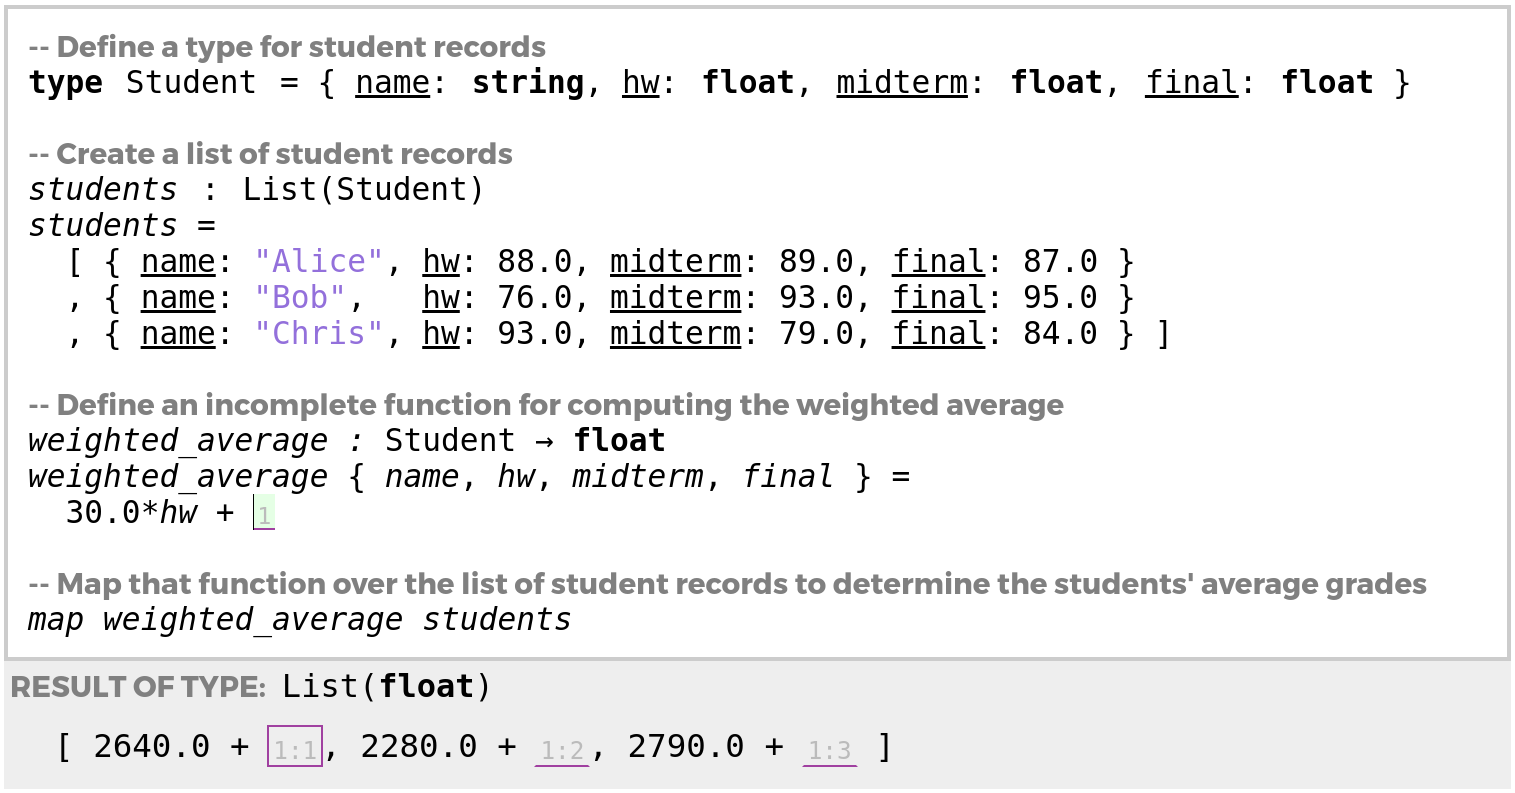
\includegraphics[width=0.8\textwidth,interpolate=false]{images/grades-cell-mockup.png}
\vspace{-3px}
\caption{Evaluating an incomplete functional program past the first hole}
\label{fig:grades-cell-mockup}
\end{subfigure}

\vspace{10px}

\begin{subfigure}[t]{\textwidth}
\centering
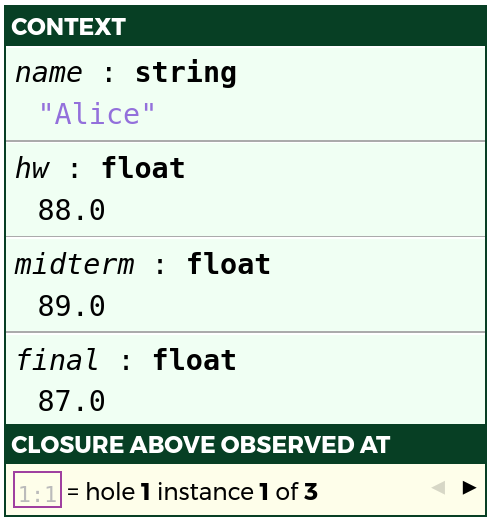
\includegraphics[width=0.29\textwidth,interpolate=false,valign=c]{images/grades-sidebar-1.png}
~${}^\blacktriangleright$
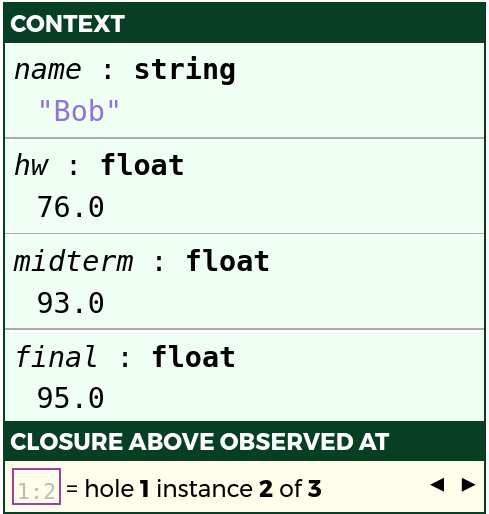
\includegraphics[width=0.29\textwidth,interpolate=false,valign=c]{images/grades-sidebar-2.png}
~${}^\blacktriangleright$
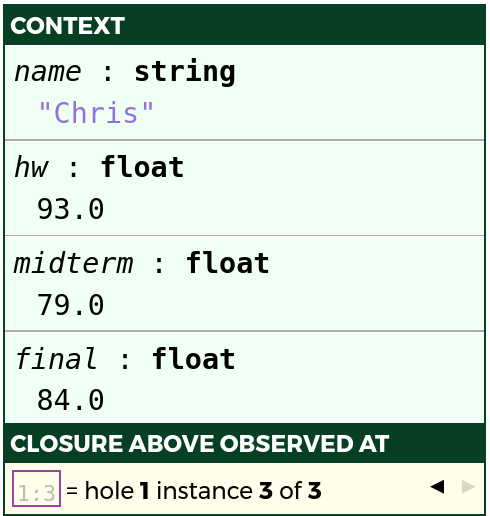
\includegraphics[width=0.29\textwidth,interpolate=false,valign=c]{images/grades-sidebar-3.png}
\caption{The live context inspector communicates relevant static \emph{and} dynamic information about variables in scope.}
\label{fig:grades-sidebar}
\end{subfigure}
% %% TODO once the code above is removed, scale up the screenshots
% 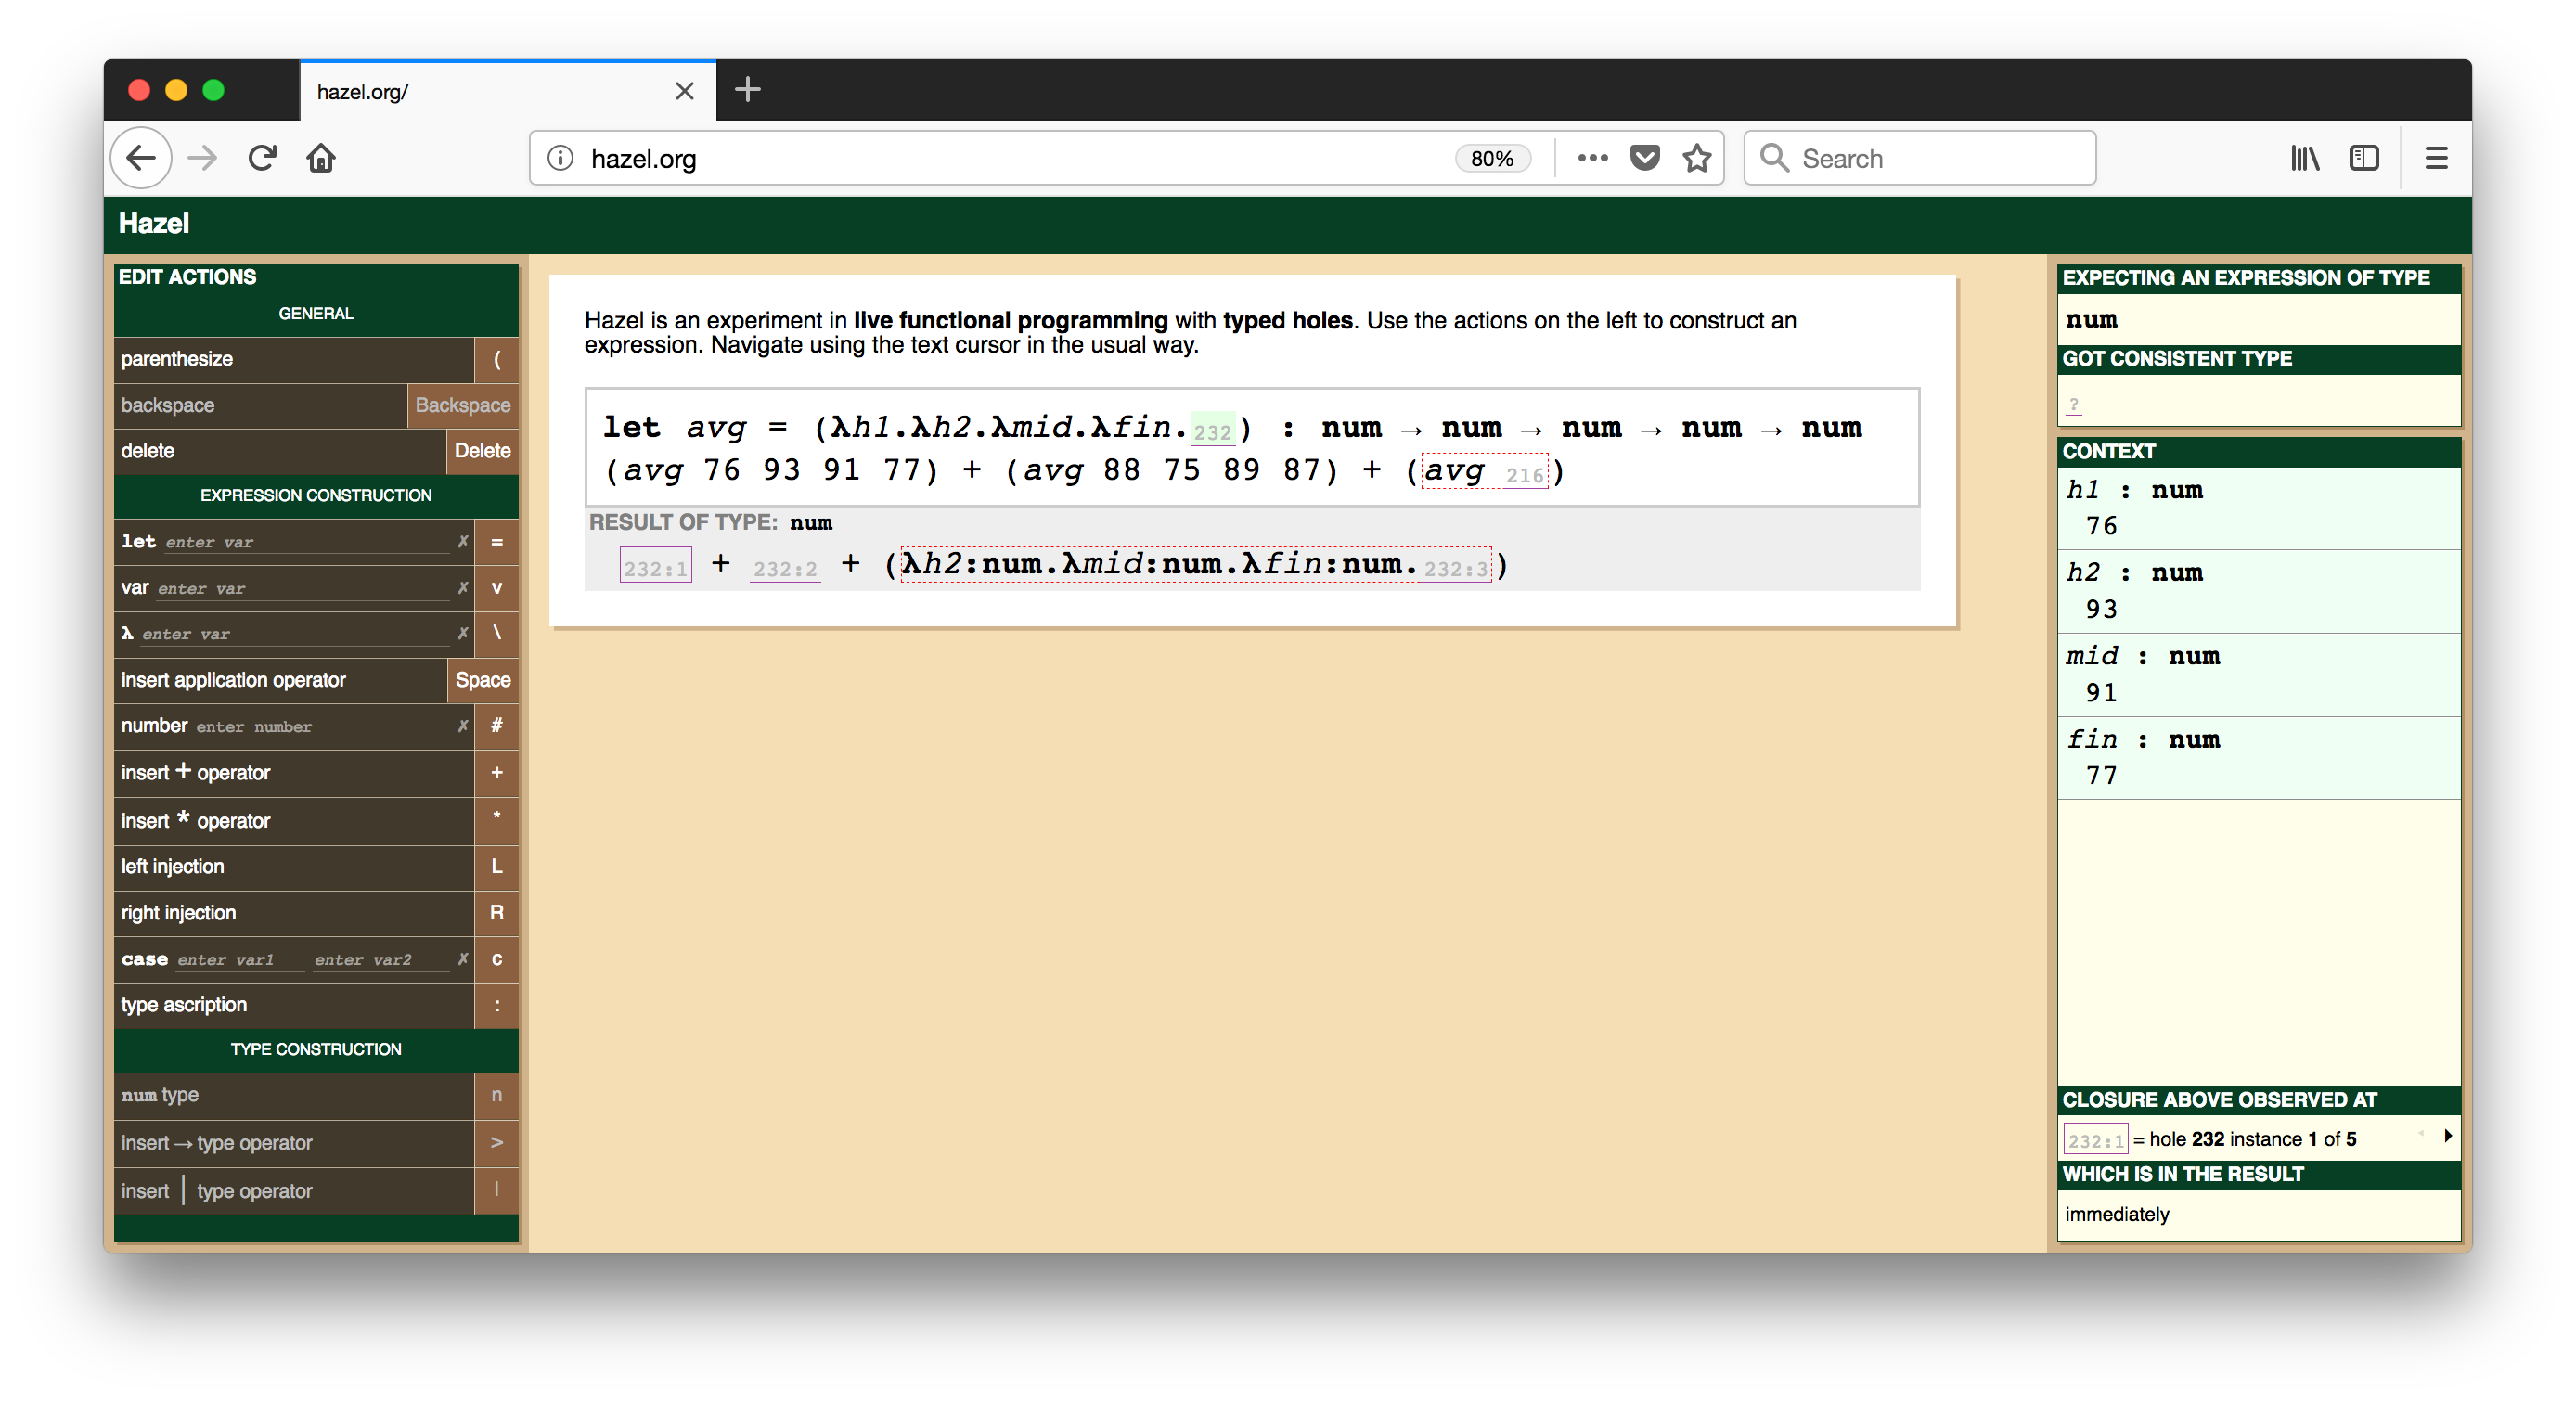
\includegraphics[scale=0.20]{images/hazel-placeholder-0.png}

% \rkc{Draw arrows and captions on the top figure to show how to get
% to the bottom figure.
% ser navigates to hole a, types + to create a plus, types * to create a
% multiplication, types \#10 to create 10, types vh1 to create variable use.}

% 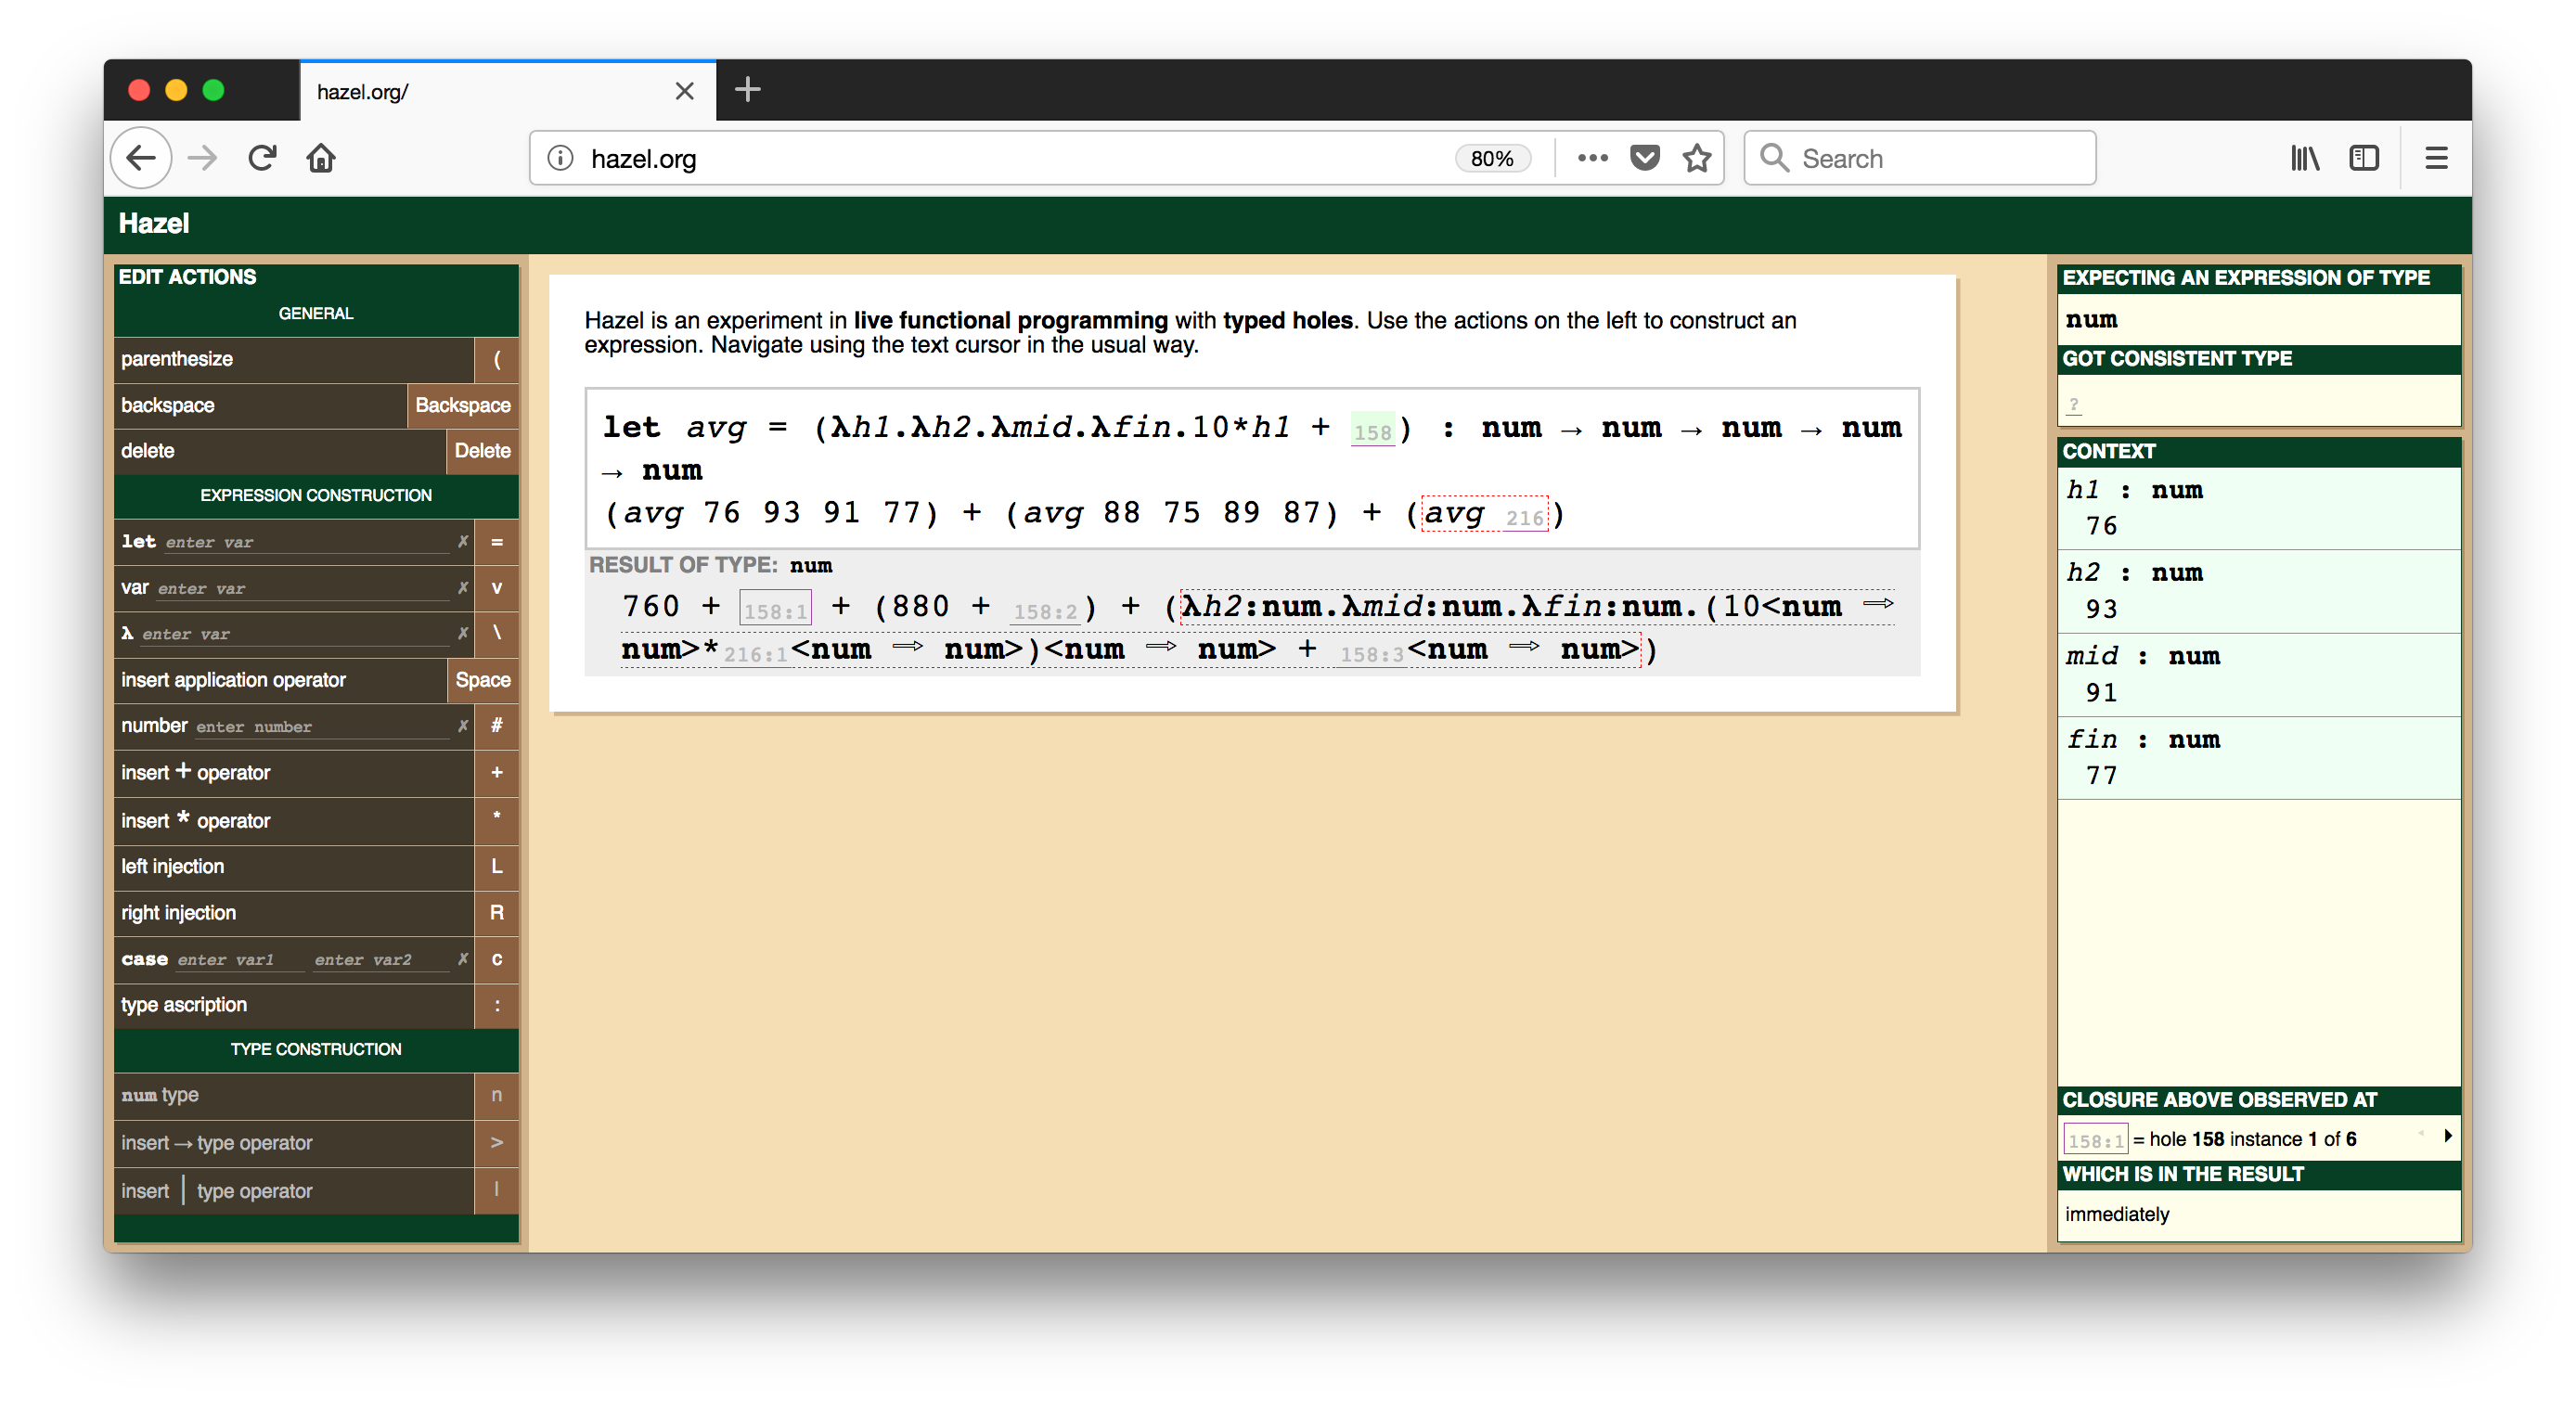
\includegraphics[scale=0.20]{images/hazel-placeholder-1a.png}
\vspace{3px}

\caption{Example 1: Grades}
\label{fig:grades-example}
\vspace{-5px}
\end{figure}



\newcommand{\overviewExample}[2]{\paragraph{Example {#1}: {#2}}}

Let us start with an example-driven overview of this paper's approach in \Hazel, a live programming environment being developed by \citet{HazelnutSNAPL}. The \Hazel user interface is based roughly on IPython/Jupyter \cite{PER-GRA:2007}, with a result appearing below each cell that contains an expression, and the \Hazel language is tracking toward feature parity with \Elm~(\url{elm-lang.org}) \cite{czaplicki2012elm,Elm}, a popular pure functional programming language similar to ``core ML'', with which we assume familiarity. \Hazel is intended initially for use by students and instructors in introductory functional programming courses (where \Elm~ has been successful \cite{DBLP:journals/corr/abs-1805-05125}). 
For the sake of 
exposition, we have post-processed the screenshots in this section after generating them in \Hazel to make use of  ``syntactic and semantic sugar'' from \Elm~that was not available in \Hazel (which, as of this writing, implements little more than the language features described in Sec.~\ref{sec:calculus} and the appendix). These conveniences are orthogonal to the contributions of this paper; all of the user interface features demonstrated in this section have been implemented and all of the computations can be expressed using standard ``encoding tricks''.

\subsection{Live Programming with Incomplete Expressions}

The process of writing new program fragments includes many states in which the
program under construction is, by definition, incomplete.
%
It is natural for a programmer to ``jump back and forth'' between different
places in the program, iteratively and alternately developing the missing
pieces.
%
The primary benefit of our approach is that such programs can be evaluated in
order to provide useful feedback during this editing workflow.

% !TEX root = hazelnut-dynamics.tex

\begin{figure}[t]
\begin{subfigure}[t]{\textwidth}
\centering
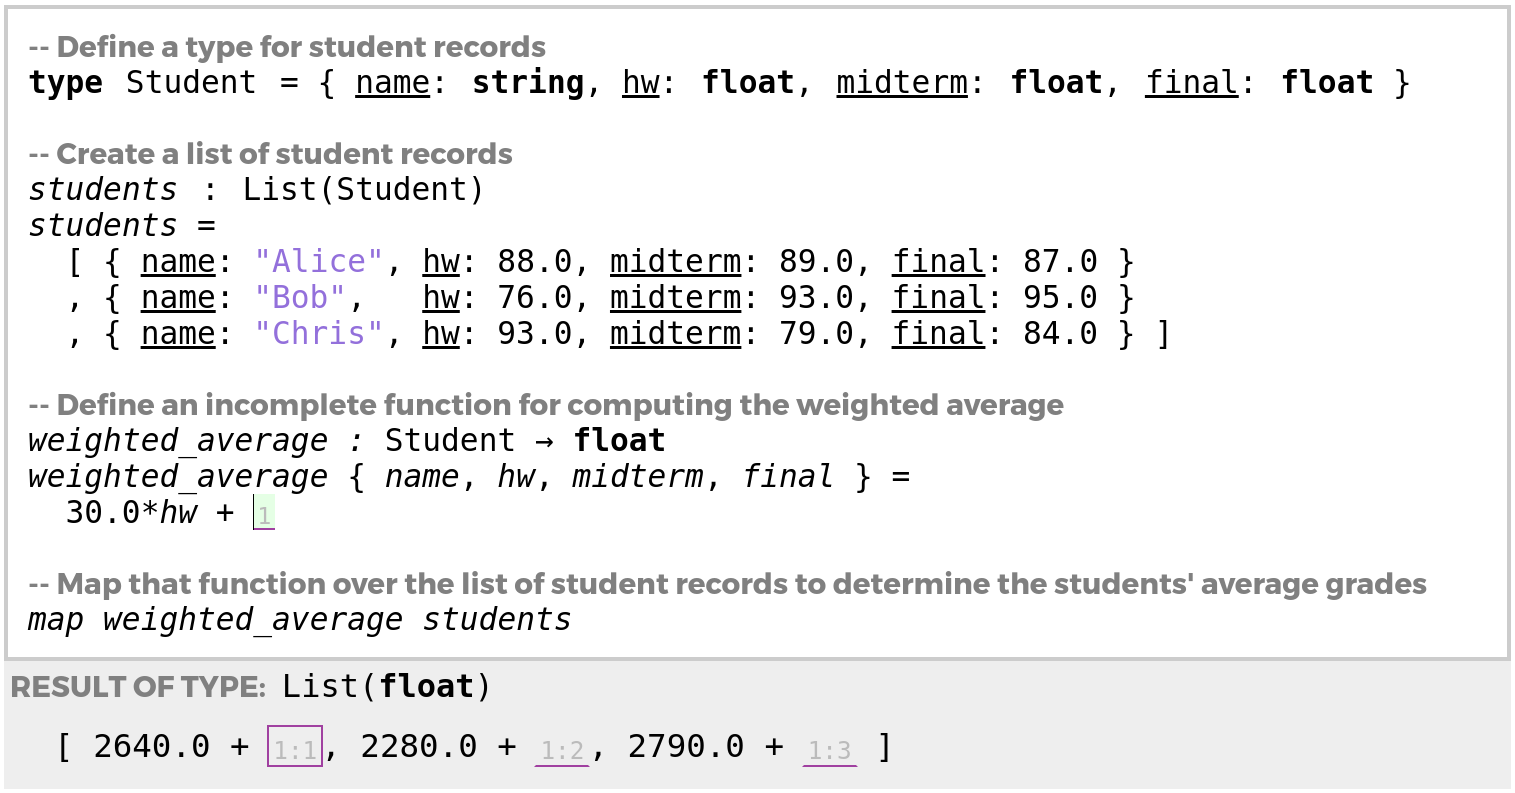
\includegraphics[width=0.8\textwidth,interpolate=false]{images/grades-cell-mockup.png}
\vspace{-3px}
\caption{Evaluating an incomplete functional program past the first hole}
\label{fig:grades-cell-mockup}
\end{subfigure}

\vspace{10px}

\begin{subfigure}[t]{\textwidth}
\centering
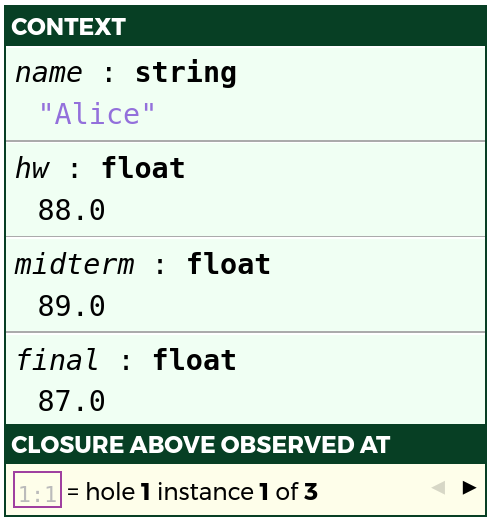
\includegraphics[width=0.29\textwidth,interpolate=false,valign=c]{images/grades-sidebar-1.png}
~${}^\blacktriangleright$
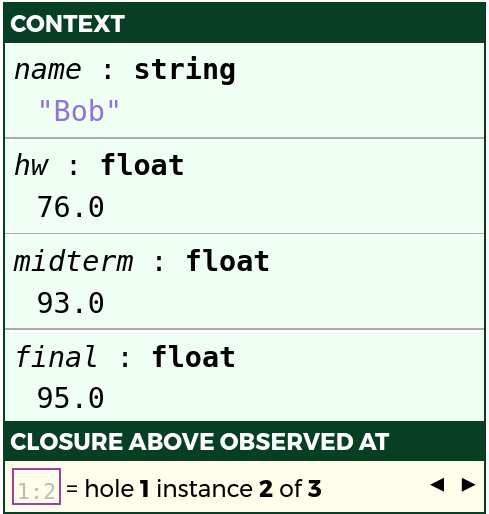
\includegraphics[width=0.29\textwidth,interpolate=false,valign=c]{images/grades-sidebar-2.png}
~${}^\blacktriangleright$
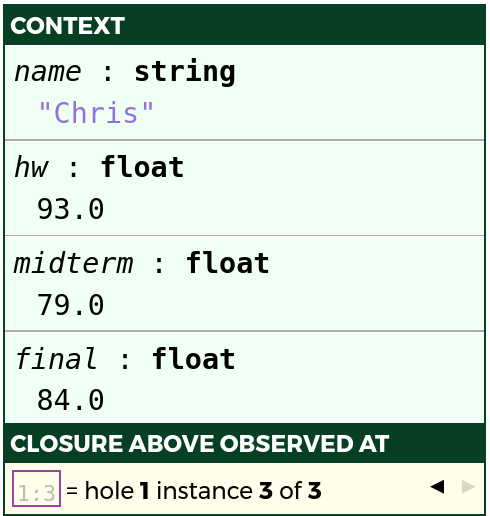
\includegraphics[width=0.29\textwidth,interpolate=false,valign=c]{images/grades-sidebar-3.png}
\caption{The live context inspector communicates relevant static \emph{and} dynamic information about variables in scope.}
\label{fig:grades-sidebar}
\end{subfigure}
% %% TODO once the code above is removed, scale up the screenshots
% 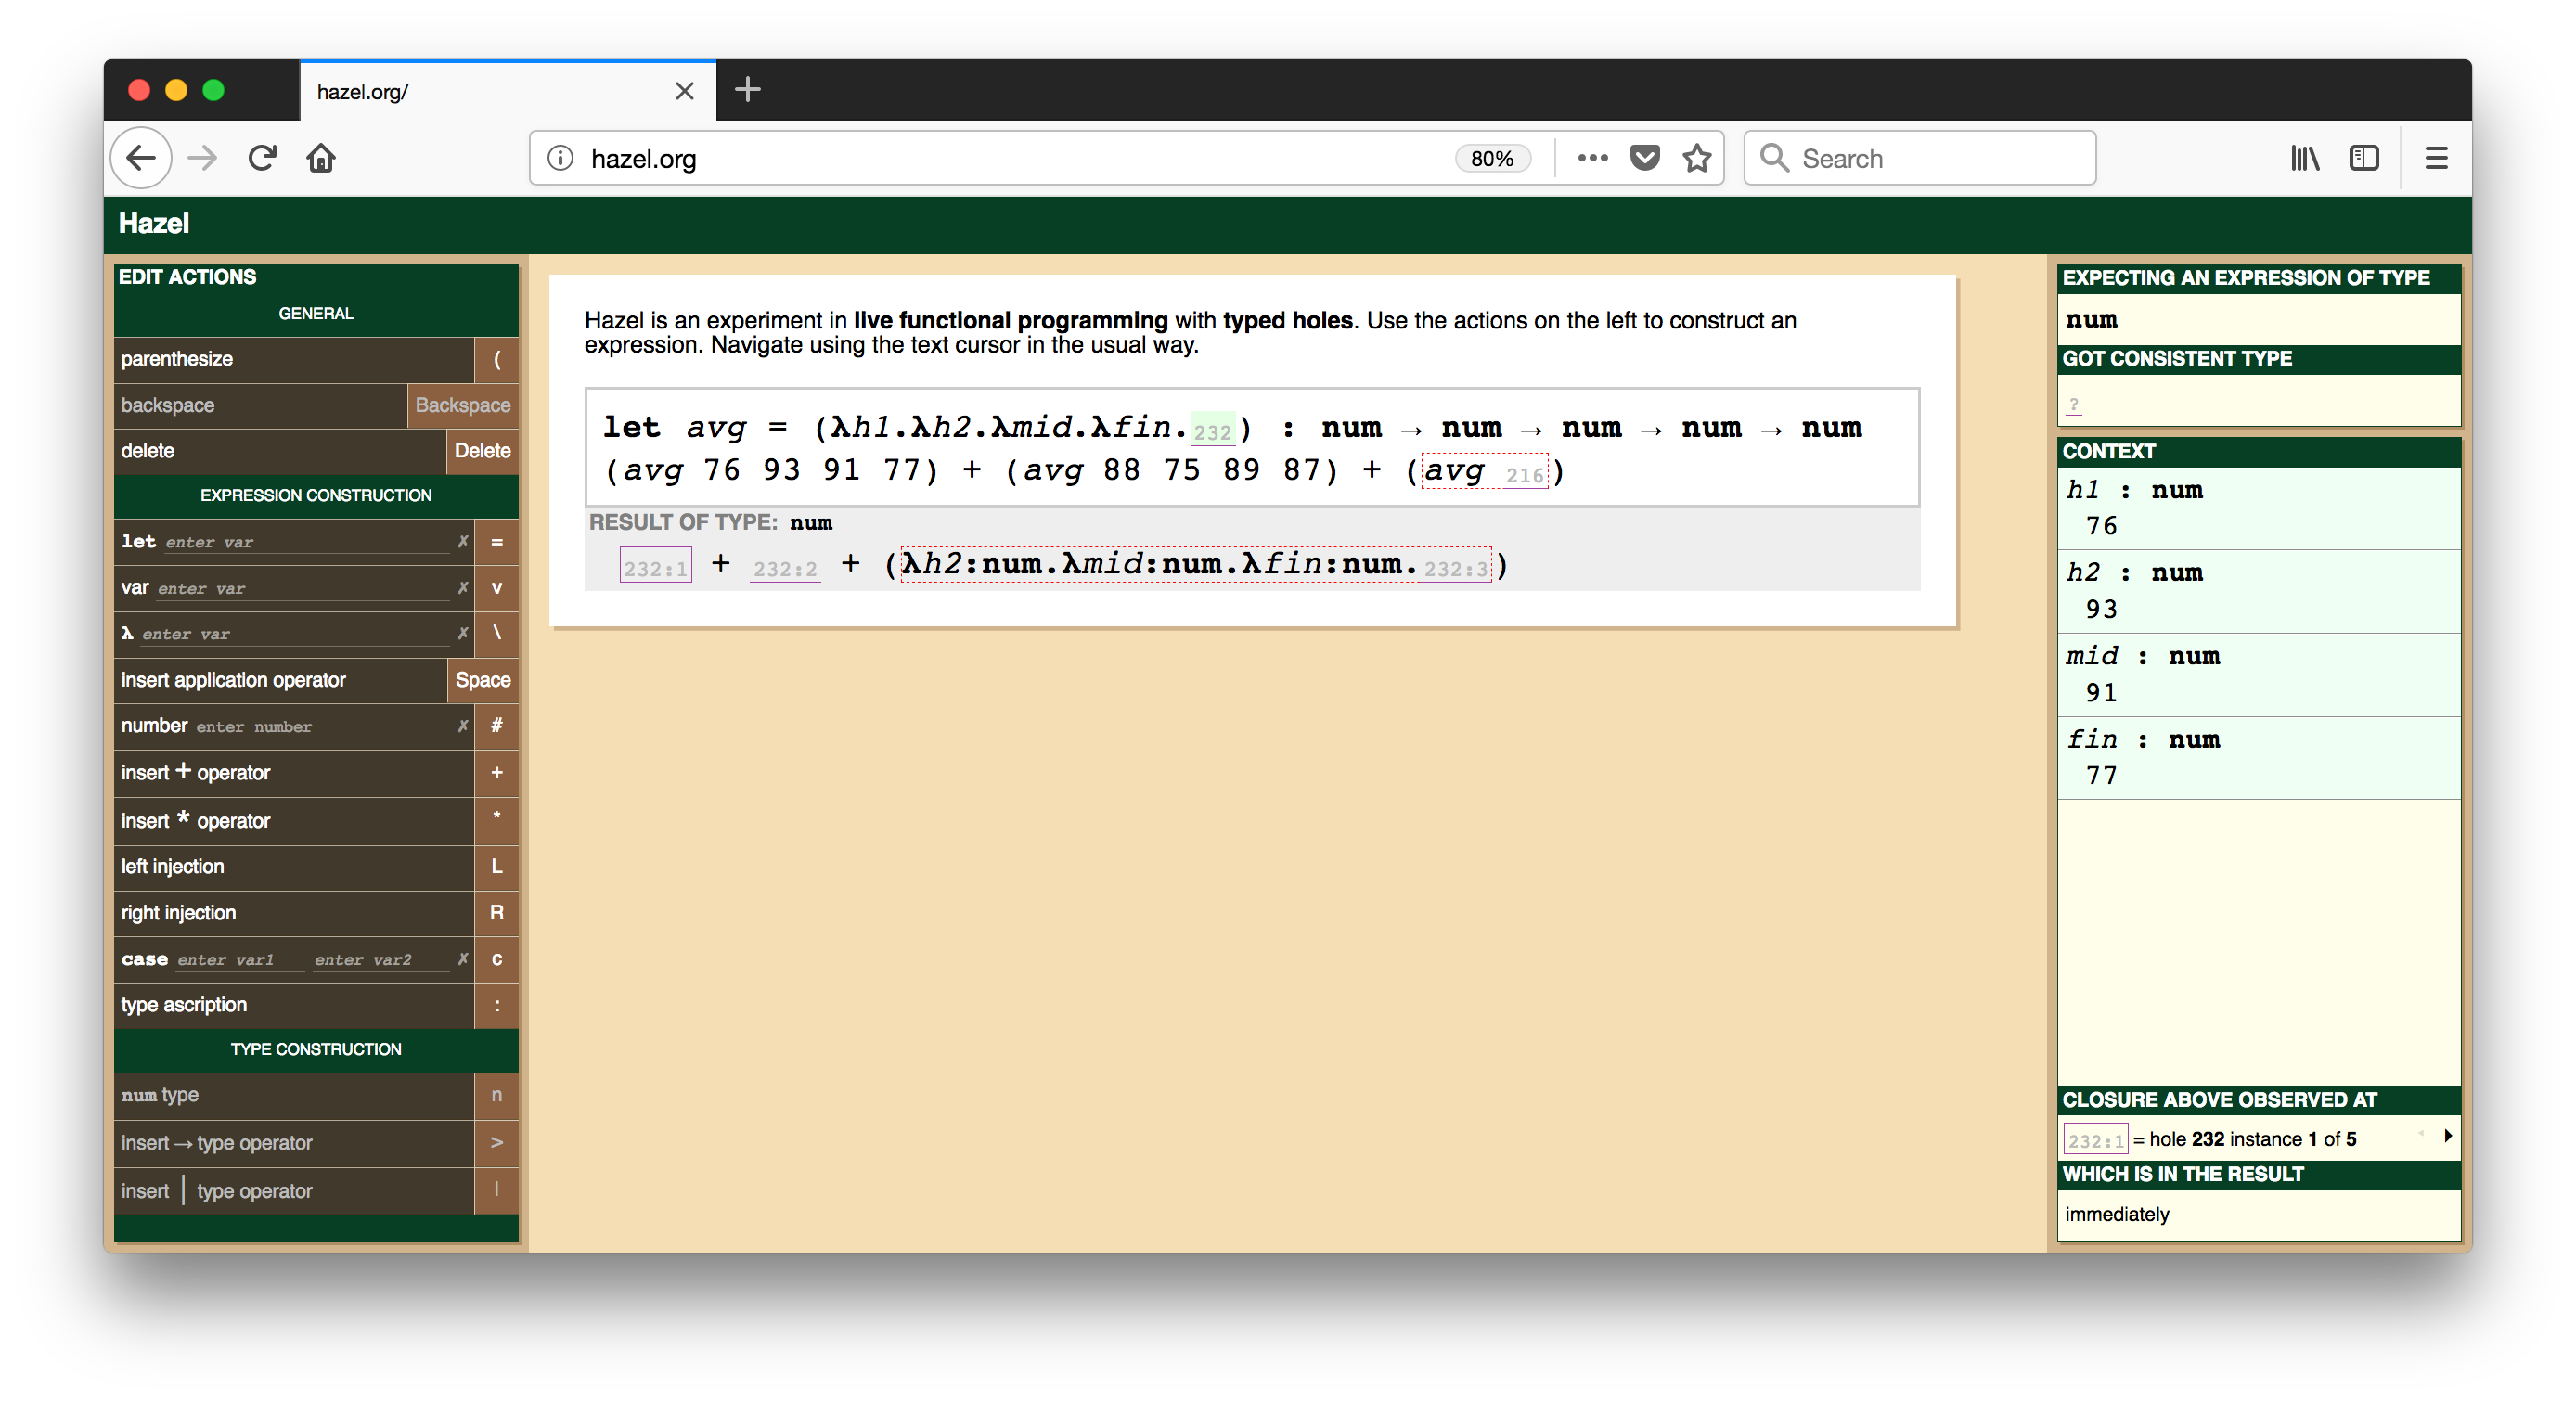
\includegraphics[scale=0.20]{images/hazel-placeholder-0.png}

% \rkc{Draw arrows and captions on the top figure to show how to get
% to the bottom figure.
% ser navigates to hole a, types + to create a plus, types * to create a
% multiplication, types \#10 to create 10, types vh1 to create variable use.}

% 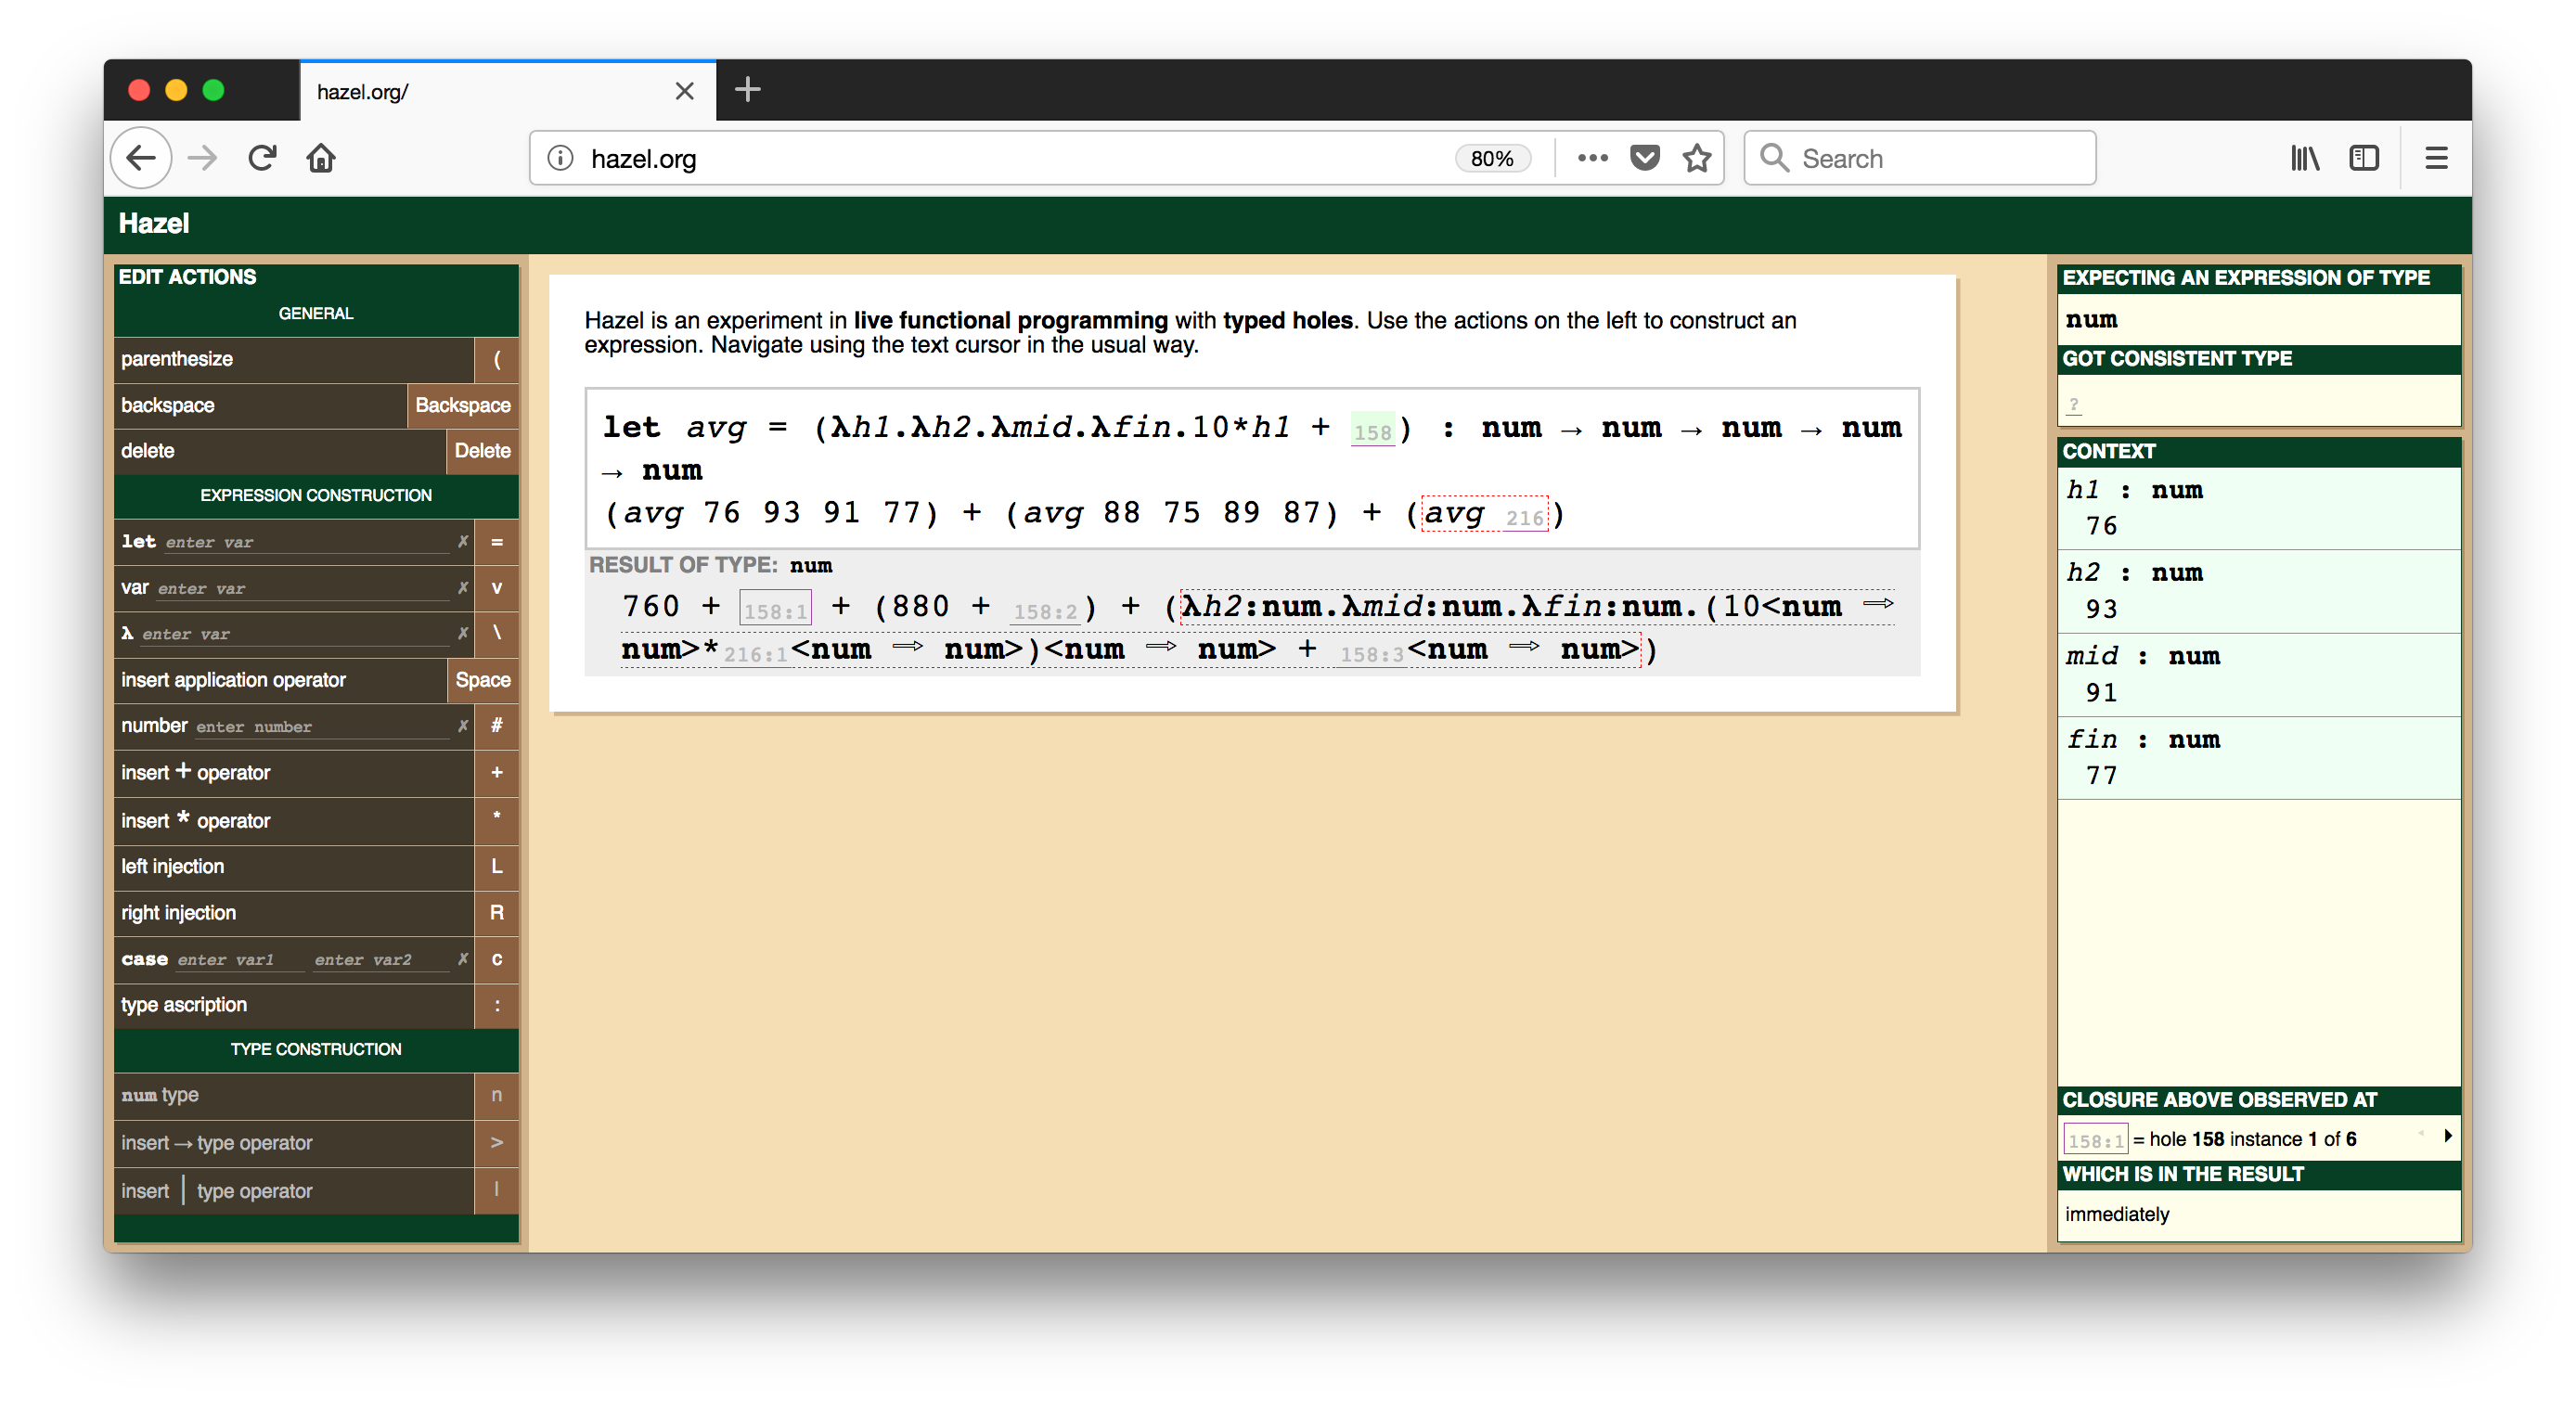
\includegraphics[scale=0.20]{images/hazel-placeholder-1a.png}
\vspace{3px}

\caption{Example 1: Grades}
\label{fig:grades-example}
\vspace{-5px}
\end{figure}


Consider a teacher who is in the midst of developing a \HazelnutLive{} notebook
(depicted in \autoref{fig:grades-example}) to compute final student grades at
the end of a term.
%
In the first cell in \autoref{fig:grades-example}, the teacher defines a record
type, \li{student_data}, for each student's course data.
%
In our simplified example, this includes the student's name, of type
\li{string}, and five grades, each of type \li{float}.

\overviewExample{1}{Computing Weighted Averages}
%
The teacher begins writing a \li{weighted_average} function that will
compute a weighted average, of type \li{float}, for each \li{student_data}
record.
%
The body of \li{weighted_average} is not yet written---marked with the
\emph{empty hole} on line \rkc{XXX}--- but the teacher jumps ahead to map the
function over the \li{grades} list.

\begin{lstlisting}
let weighted_average(g: student_data) =
  ??;

let weighted_averages = List.map weighted_average grades;
\end{lstlisting}

\noindent
%
\HazelnutLive{} evaluates this incomplete program, showing its
\emph{indeterminate} result in the sidebar on the right half of
\autoref{fig:grades-example}; this value is a list whose length is the same as
\li{grades}, where each element is the (indeterminate) result of evaluating the
hole expression inside \li{weighted_average}.
%
Notice that the hole on line \rkc{XXX} is assigned a unique static identifier
(\ie{}~\li{a}) and that the indeterminate results it produces are assigned
corresponding unique dynamic identifiers (\ie{}~\li{a.1}, \li{a.2}, etc.).
%
In contrast, the typical ad-hoc approach to simulating hole expressions, namely,
using placeholder expressions like \li{raise "Not yet implemented."}, would halt
the program as soon it is evaluated (in this case, inside the definition of
\li{List.map} when the function is applied to the first element of \li{grades}.
%
By ``evaluating around'' the hole in \HazelnutLive{}, the programmer can at
least see that the resulting expression does indeed evaluate to a list with the
correct number of (indeterminate) values.

Now the teacher returns to \li{weighted_average} to work on the missing
expression, with the goal of computing a weighted sum of each of a student's
grades.
%
The teacher uses a \HazelnutLive{} edit action to create a sum expression,
filling in the first summand by weighting the \li{hw1} score to account for 10\%
of the weighted average; the rest of the computation is a new hole expression
(\li{??_b}), yet to be filled in.

\begin{lstlisting}
let weighted_average(g: student_data) =
  (10.0 *. g.hw1) +. ??_b;
\end{lstlisting}

\noindent
%
\HazelnutLive{} immediately runs this incomplete program, displaying the updated
list of indeterminate expressions \li{[760.0 + ??_b.1, 880.0 + ??_b.2, ...]}.
%
Right away, the teacher recognizes that the values are too large; they should be
at most \li{100.0}.
%
The teacher realizes that representing percentage points as \li{float}s requires
that the constant on line \rkc{XXX} ought to be \li{0.10} instead.
%
Because of this live feedback, the teacher corrects this error right away and
avoids making similar programming errors in the rest of the calculation.
%
The teacher continues to build the rest of the arithmetic expression until it is
complete (there are no longer any expression holes), and the result of
immediately running the finished program shows that each of values in the final
result list is in the range \li{0.0} to \li{100.0}.

\overviewExample{2}{Assigning Letter Grades}
%
The teacher's next task is to map the weighted averages to the letter grades A
through F (we will consider only ``whole'' letter grades, for simplicity).
%
The \li{grade_cutoffs} record type describes the minimum cutoff for each of
these six possible grades.
%
Initially, each value in the \li{cutoffs} record is a hole.

\begin{lstlisting}
type grade_cutoffs =
  { a: float, b: float, c: float, d: float, f: float };

let cutoffs =
  { a = ??_a, b = ??_b, c = ??_c, d = ??_d, f = ??_f };
\end{lstlisting}

\noindent
%
%% initially all holes, because it will be different year-to-year based on the %
%data, differences in course difficulty, and to satisfy fairness criteria.
%
Before starting to fill in the cutoffs, the teacher jumps ahead to write a
function \li{letter_grade} that will make the connection between \li{cutoffs}
and \li{weighted_averages}.
%
Because she intends to look at the data to help select the cutoff values, the
teacher sorts the \li{weighted_averages} and then maps them to
\li{letter_grades}.

\begin{lstlisting}
let letter_grade(n: weighted_average) =
  if n >= cutoffs.a then "A" else
  if n >= cutoffs.b then "B" else
  if n >= cutoffs.c then "C" else
  if n >= cutoffs.d then "D" else
  if n >= cutoffs.f then "F" else "Incomplete";

let sorted_weighted_averages = List.sort weighted_averages;

let letter_grades = List.map letter_grade sorted_weighted_averages;
\end{lstlisting}

\noindent
%
When \HazelnutLive{} runs this program, the guard of the outermost conditional
(\li{n >= cutoffs.a} on line \rkc{XXX}), is indeterminate because \li{cutoffs.a}
is.
%
Therefore, each of the indeterminate expressions in \li{letter_grades} is the
entire expression body, albeit with different bindings for \li{n}.
%
Displaying such ``large'' indeterminate expressions can quickly consume all
available screen space, overwhelming the user with too much information.
%
\autoref{fig:XXX} shows how \HazelnutLive{} renders large indeterminate
expressions (\ie{}~anything other than ``small'' indeterminate value (a constant
or hole) or list of small values) simply as \li{..} to save space.
%
Hovering over this abbreviation (as shown in \autoref{fig:XXX} displays the full
indeterminate expression---as well as the evaluation environment that surrounds
it---as a tooltip.
%
\autoref{sec:discussion} discusses this and other user interface concerns when
trying to display useful live feedback without overwhelming the user.
%
These usability factors are beyond the scope of our work, which is to define
semantic foundations on which such user interfaces can be built.

To start deciding \li{cutoffs}, the teacher looks at the \li{weighted_averages}
sorted in descending order.
%
The data shows a natural gap between \li{92.2} and \li{89.5}.
%
So, she chooses to use \li{92.0} as the cutoff for A.
%
Resuming the computation from before, \HazelnutLive{} resolves the conditional
expressions for the first \rkc{XXX} indeterminate expressions, because each of
those \li{n} values was greater than \li{cutoffs.a}.
%
The remaining \rkc{XXX} expressions also proceeded to evaluate the first guard,
and are now indeterminate at the guard for the second conditional.

Before assigning other cutoff values, the teacher would like to get a sense of
whether this first choice is a good one.
%
She jumps ahead to to write a function that computes the distribution of letter
grades.

\begin{lstlisting}
let compute_distribution(list: list(float)) =
  let n = List.length letter_grades in
  List.map
    (\x -> (x, showPercentage (List.length (List.filter ((==) x) list)) /. n))
    ["A","B","C","D","F","Incomplete"];

let distribution = compute_distribution(letter_grades);
\end{lstlisting}

\noindent
%
Running \li{compute_distribution} shows that the percentage of As is
\rkc{XXX\%}, which is smaller than what the teacher would like;
the remaining percentages are all indeterminate.
%
Returning to the value of \li{sorted_data}, she sees a cluster around \li{89.0}
and then another gap between \li{88.2} and {85.5}.
%
So, the teacher adjusts \li{cutoffs.a} to be \li{88.0}.
%
Because this edit is outside of a hole expression, \HazelnutLive{} discards the
previous execution state and reevaluates the entire program.
%
Existing techniques for incremental computation~\cite{XXX,XXX}, however, could
be applied to seek opportunities for reuse even when non-hole expressions are
modified.
%
Because the focus of work is on the novel implications of running programs with
holes, our calculus and implementation supports caching ``edit-and-resume'' only
for the novel situation in which evaluation proceeds around holes.
%
After re-evaluation, the percentage of As becomes \rkc{XXX\%}, which better
matches the teacher's intention.

In this fashion, the teacher continues down the list of sorted averages,
determining appropriate values for each cutoff.
%
Whenever the teacher is only filling in the ``next'' cutoff, the computation
from before can simply be resumed.
%
Overall, throughout the workflow described in these two examples, the programmer
can continue to evaluate the program, and receive meaningful feedback, while
going back and forth between different pieces under development.

% !TEX root = hazelnut-dynamics.tex

%% \subsection{Live Programming with Type Errors}

\subsection{Example 3: Live Programming with Static Type Errors}
\label{sec:static-errors}


% \begin{subfigure}[t]{\textwidth}
\begin{figure}
\centering
\includegraphics[width=0.95\textwidth,interpolate=false,valign=t]{images/qsort-type-error-inset.png}
% 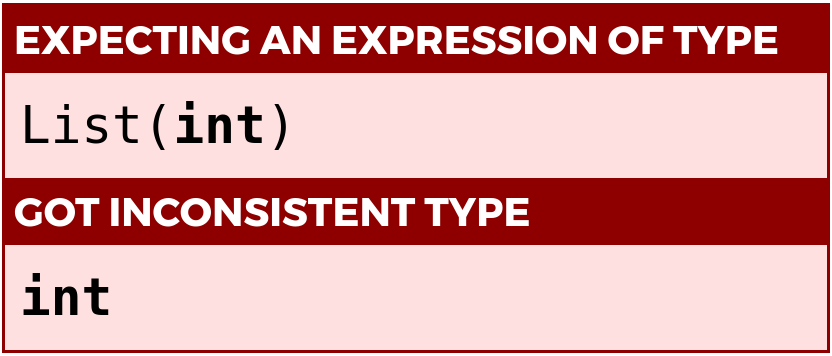
\includegraphics[width=0.28\textwidth,interpolate=false,valign=t]{images/type-inconsistency.png}
\vspace{2px}
\caption{Example 3: Ill-Typed Quicksort}
\label{fig:qsort-type-error}
\vspace{-3px}
\end{figure}
% \end{subfigure}


The previous examples were incomplete 
because of \emph{missing} expressions.
%
Now, we discuss programs that are incomplete, 
and therefore conventionally meaningless, because of
\emph{type inconsistencies}. 
%
Let us return to the quicksort example just described, 
but assume that the programmer has filled in the previous hole
as shown in Fig.~\ref{fig:qsort-type-error}. In Sec.~\ref{sec:resumption}, we discuss
how the programming environment could avoid restarting evaluation after such edits by using the values stored in the hole closures.

The programmer appears to be on the right track conceptually
in recognizing that the pivot needs to appear between the 
smaller and bigger elements. 
However, the types do not quite work out: the \li{@} operator here
performs list concatenation, but the pivot is an integer. 
Most compilers and editors will report a static error message
to the programmer in this case, and \Hazel 
follows suit in the type inspector (shown inset in Fig.~\ref{fig:qsort-type-error}). 
However, our argument is that the presence of a static type error should not cause all feedback about 
the dynamic behavior of the program to ``flicker out'' or ``go stale'' --
after all, there are perfectly meaningful parts of the program (both nearby
and far away from the error) 
whose dynamic behavior may be of interest. Concrete results can also help the programmer understand the implications of the type error \cite{Seidel2016}.
% After all,
% the error is localized and there is perfectly good code elsewhere 
% in the program (if not nearby, then perhaps far away).

Our approach, following the prior work of \citet{popl-paper}, 
is to semantically internalize the ``red outline'' around
a type-inconsistent expression as a \emph{non-empty hole} around that expression.
Evaluation safely proceeds past a non-empty hole just as if it were an empty hole.
The semantics also associates an environment with each instance of a non-empty hole,
so we can use the live context inspector essentially as in Fig.~\ref{fig:qsort-sidebars} (not shown). 
Evaluation proceeds inside the hole, so that 
feedback about the type-inconsistent expression, which might ``almost'' be correct, is available. 
In this case, the result at the bottom of Fig.~\ref{fig:qsort-type-error}
reveals that the programmer is on the right track: the list elements 
appear in the correct order.
They simply have not been combined correctly.

We are treating \li{@} as a primitive operator in this example. If it were defined as a function, then
it would be possible to further reduce the example by proceeding into the function body. This is likely unhelpful for
functions other than those that programmer is actively working on. Our semantics \emph{allows} beta reduction when the argument is a hole, but it does not \emph{require} it.

Although \Hazel inserts non-empty holes automatically, the earlier work on \Hazelnut allowed the programmer to explicitly insert non-empty holes. It may be that these are useful even when there is not a type inconsistency because the non-empty hole defers elimination of the enclosed expression and causes hole closure information to be tracked. For example, if we repaired the program in Fig.~\ref{fig:qsort-type-error} by replacing the erroneous variable \li{pivot} with \li{[pivot]} and then inserted a non-empty hole around this expression, the result would show all of the list concatenation operations that would be performed without actually performing them, producing a result much like that in Fig.~\ref{fig:qsort-type-error}. This provides another way to explore the recursive structure of the \li{qsort} function.

% For example, consider the following two definitions.

% \begin{lstlisting}
% let bad_bool : bool = ?? 0 ??_bad_bool;

% let bad_int : int = 1 + ?? true ??_bad_int_second_argument;
% \end{lstlisting}

% \noindent
% %
% These two definitions are ill-typed under standard typing disciplines.
% %
% In contrast, \citet{popl-paper} present a bidirectional type system that assigns
% types to both, by wrapping type-inconsistent expressions (\li{0} on line
% \rkc{XXX} and \li{true} on line \rkc{XXX} above) in \emph{non-empty} holes.
% %
% Non-empty holes prevent local type inconsistencies from polluting the rest of
% the program surrounding it, which may or may not itself contain additional
% inconsistencies.

\begin{comment}
\overviewExample{2}{Sum List}
%
Consider the following buggy program (observed during an undergraduate
functional programming course~\cite{Seidel2016}) that attempts to sum a list
integers.
%
The error is that the base case produces a list rather than an integer.

\begin{lstlisting}
sum_list : list(int) -> int
sum_list [] = ?[]?
sum_list (n:ns) = n + sum_list ns
\end{lstlisting}

\noindent
%
Because the list expression on line 2 does not have type \li{int} as required,
it is wrapped in a (non-empty) hole by the bidirectional type
checker~\cite{popl-paper}.
%
Rather than trying to debug the error based on the static error, the programmer
may wish to trying running the function anyway by calling, say, \li{sum_list(2)}.
%
\HazelnutLive{} runs and produces the indeterminate expression \li{3 + ?[]?}.
%
By observing that the hole expression is being added to the integer \li{3}, he
realizes that it needs to be an integer, specifically, \li{0}.
%
Compared to the trace displayed by \citet{Seidel2016}, the indeterminate result
produced by \HazelnutLive{} is ``flattened'' because the expression \li{1 + 2}
successfully proceeded to evaluate despite the error elsewhere.
\end{comment}

%% TODO fold error from Erwig paper.
%% %
%% see that final call on stack does have the right answer, but
%% it's wrapped in a singleton list when the expected type is not
%% a list.
%% %
%% fix is to remove the list, the rest of the computation remains
%% the same, but b/c they were all wrapped in holes, need to re-run.
%% %
%% (add some mechanism for type-consistent non-empty-holes...)

\begin{comment}

\overviewExample{4}{Stutter}
%
Consider the following function which attempts to produce a
list where every element is repeated twice (borrowed from \citet{Osera2015}).
%
The combiner function to \li{List.foldr} needs to produce a \li{list(int)}, but
it produces a \li{list(list(int)} instead.

\begin{lstlisting}
stutter : list(int) -> list(int)
stutter xs = List.foldr (\x acc -> ?[x,x]? : acc) [] xs
\end{lstlisting}

\noindent
%
The bidirectional type checker of \citet{popl-paper} wraps the expression
\li{[x,x]} inside a non-empty hole.
%
%% The editor has a choice about which expression to ``blame'' for the error; the
%% entire application that forms the body of the lambda is analyzed against the
%% return type \li{list(int)}, so that is a reasonable choice for the editor to
%% make; another would be to assume that the arguments \li{[x,x]} and \li{acc} are
%% both as intended and that only the function \li{(:)} is type-consistent.
%% %
%% Although one could imagine a setting in which a user would perform this
%% reasoning, let's assume the simplest approach for marking consistencies that
%% wraps the entire application.
%
Running this on \li{stutter [1,2,3]} produces the indeterminate result

\begin{lstlisting}
?  [1,1] : (? [2,2] : (? [[3:3]] ?) ?) ?,
\end{lstlisting}

\noindent
%
which shows the unfolding of \li{List.foldr}.
%
We refer to nested indeterminate computations like this as \rkc{\emph{hole
environment traces} or \emph{hole environment trees}}.
%
The result of the innermost indeterminate expression is \li{[[3,3]]}.
%
The user realizes that there are too many levels of nesting, so
he replaces the \li{(:)} with \li{(@)}, which addresses the type inconsistency
and, when reevaluated, produces the desired result.

\end{comment}

% !TEX root = hazelnut-dynamics.tex

\subsection{Example 4: Type Holes and Dynamic Type Errors}
\label{sec:dynamic-type-errors}

% \begin{subfigure}[t]{\textwidth}
\begin{figure}
\centering
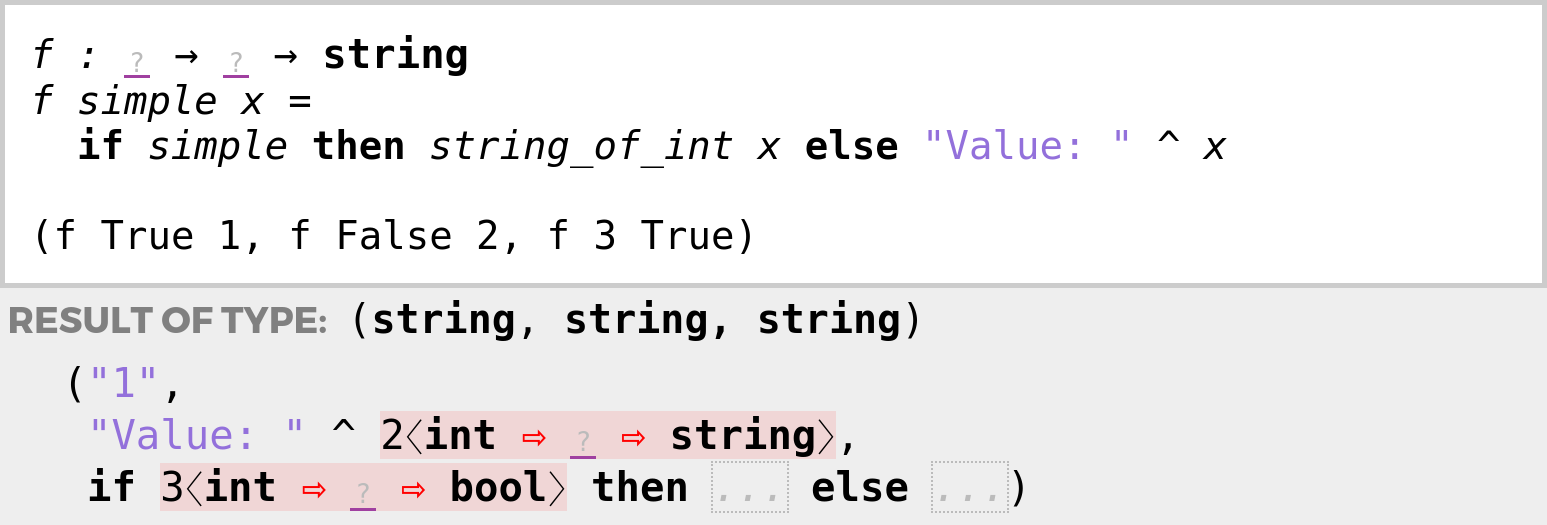
\includegraphics[width=0.73\textwidth,interpolate=false,valign=t]{images/cast-errors.png}
% 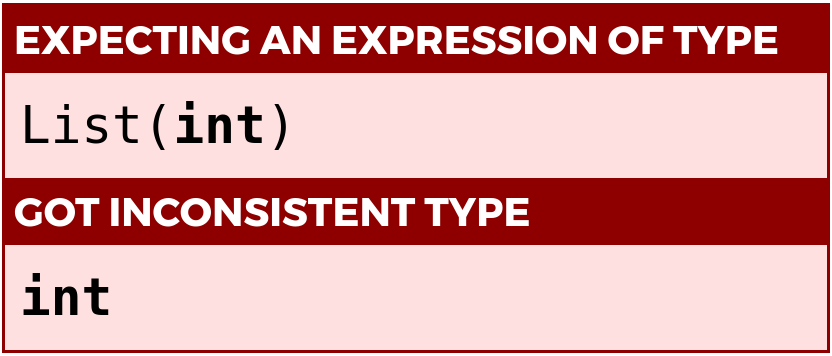
\includegraphics[width=0.28\textwidth,interpolate=false,valign=t]{images/type-inconsistency.png}
\caption{Example 4: Type Holes and Dynamic Type Errors}
\label{fig:cast-errors}
\vspace{-6px}
\end{figure}
% \end{subfigure}


% So far, we have only discussed incomplete programs where a hole appears within an expression.
In \Hazel, the program can also be incomplete because holes appear in types. 
\citet{popl-paper} confirmed that the literature on \emph{gradual type systems} \cite{Siek06a,DBLP:conf/snapl/SiekVCB15} is directly relevant to the problem of reasoning statically with type holes, by identifying the type hole with the unknown type. 
Unsurprisingly, then, it is also relevant to the problem of running 
programs with type holes. Indeed, that is the purpose of gradual typing: to be able to run programs that are not yet sufficiently annotated with types by inserting \emph{casts} only where necessary. As such, let us consider only a small synthetic example to demonstrate what is unique to our approach.

Fig.~\ref{fig:cast-errors} defines a simple function, \li{f}, of two arguments. 
The type annotation on the first line leaves the type of those arguments unknown. 
As such, the \Hazel type system, following the gradual typing approach,
allows the body of the function to use those two
arguments at any type at all (that is, the hole type is universally consistent). 
In this case, the first argument, \li{simple}, is used at one type, \li{bool}, 
and the second argument, \li{x}, is used at two different types in the two branches (perhaps because the programmer made a mistake), 
first as an \li{int} and second as a \li{string}  (we use \li{^} for string concatenation).
Although \Hazel supports only local type inference as of this writing, 
a system that uses ML-style type reconstruction to fill type holes statically, like GHC Haskell, would only be able to fill the first hole. Leaving the second hole unfilled is 
a parsimonious alternative to arbitrarily or heuristically\todo{cite error localization papers?}{} choosing one of the possibilities and marking the
other uses of \li{x} as ill-typed.

At the bottom of the cell in Fig.~\ref{fig:cast-errors}, we have three 
example applications of \li{f}. In this case, we simply tuple the results, but we could also
have made them into tests or put them into separate cells. All three are statically
well-typed, again because the hole type is universally consistent.
The result at the bottom of Fig.~\ref{fig:cast-errors} demonstrates that the first application
of \li{f} is dynamically unproblematic. This might help the programmer confirm that at least
the first branch of the function body has been implemented as intended without the need to comprehensively
address all of the problems in the program. This flexibility is a common motivation for dynamic languages in programming folklore.

The second application of \li{f}, in contrast, causes a dynamic type error because the second argument, \li{2}, is an \li{int} but evaluation takes the branch where \li{x} is used as a \li{string}. 
Rather than aborting evaluation immediately when this occurs, as in existing gradual type systems, the problematic sub-term becomes a \emph{failed cast} term, shown shaded in red, which can be read ``\li{2} is an \li{int} that was used through a variable of hole type (\li{?}) as a \li{string}''. 
A failed cast behaves much like a non-empty hole in that it simply becomes an opaque value of the target type, \li{string}, that causes the surrounding concatenation operation to become indeterminate. 
Evaluation can continue on to the third application of \li{f}, which again is problematic, this time because the first argument is not a \li{bool} (perhaps because the programmer had an incorrect understanding of the argument order). 
Again, this causes a failed cast to appear, this time in guard position. Like a hole in guard position, evaluation cannot determine which branch to take so the whole guard expression becomes indeterminate. 
The pretty printer
hides the two branches behind ellipses.

In this synthetic example, it might have only been a small burden for the programmer to provide the intended types in the signature of \li{f}, but there are situations (e.g. during rapid prototyping or a live performance) where the programmer may consider the burden more substantial. This approach ensures that dynamic feedback does not have gaps even when there is a dynamic type error.

\subsection{Design Variations}


\begin{comment}
\emph{Gradual type systems}~(\eg{}~\cite{XXX,XXX,XXX}) can statically accept
programs that would otherwise be rejected by static type systems---either
because type inference cannot reconstruct a valid type assignment, or because
there may not be a unique valid type assignment at all.
%
In either case, gradual type systems allow types to contain \emph{unknown
types}, and partially unknown types can be used in contexts that require
different types, so long as they are \emph{consistent} (intuitively, equal
modulo the unknown parts).
%
Dynamic casts are then inserted to ensure that these remaining static
discrepancies are not violated at run-time.

\HazelnutLive{} inherits the notion of \emph{type holes} from
\citet{popl-paper}, which serves a similar static purpose as the unknown type in
gradual type systems.
%
In contrast to prior gradually typed languages, however, \HazelnutLive{} can
evaluate ``around'' cast errors in the same way as it does for expression holes.

\overviewExample{3}{Dynamically Typed Negation}

Consider the \li{negate} function (adapted from \cite{ChughPOPL2012}), which
cannot be assigned a static type in a conventional type system---either a
bidirectional one, like in \HazelnutLive{}, or one with ML-style,
unification-based inference---because the argument \li{x} is used at type
\li{int} on line \rkc{XXX} and \li{bool} on line \rkc{XXX}.
%
Therefore, the declared type of \li{x} is the hole type \li{??}, which allows
\li{x} to be used at the conflicting types, with each use expanded into an
expression wrapped in a \emph{cast} that will dynamically check for safety.
%
The return type also uses the hole type \li{??}, leading to additional casts in
the expansion.

\begin{lstlisting}
negate : bool -> ?? -> ??
negate b x =
  if b
    then 0 - x     // expanded to: (0 - (x<?? => int>))<int => ??>
    else not x     // expanded to: (not (x<?? => bool>))<bool => ??>

(negate false 1) + 2 + 3 + (negate true 4)
\end{lstlisting}

\noindent
%
As in prior gradually typed languages~\cite{XXX},
evaluating the expression \li{negate false 1} on line \rkc{XXX} leads to
\li{(not (1<int => ??><?? => bool>))<bool => ??>}, where the inner casts
lead to the \emph{cast error} \li{1<?? =/=> bool>} because \li{1} cannot be
safely treated as having type \li{bool}.
%
Unlike in prior gradually typed languages, however, \HazelnutLive{} evaluates
around the cast error, making progress on the \li{2 + 3 + negate false 4}
expression that surrounds the error; the final indeterminate result is
\li{(not (1<?? =/=> bool>))<bool => ??> + 1}.
%
Just like it is useful for static type checkers to report multiple errors, our
approach allows us to report multiple dynamic cast errors, and otherwise make
progress on expressions that do not depend on failed casts.
%
This approach can be incorporated into existing gradually typed languages.
\end{comment}
\begin{comment}
\subsection{Live Programming for Debugging}

Previous examples highlighted how running different kinds of incomplete
programs---ones with missing expressions, type-inconsistent expressions, or
missing types---can be useful.
%
Our final example demonstrates how expression holes may be useful even for
complete programs, in order to facilitate debugging and program understanding.

%% \overviewExample{6}{\rkc{...}}
%%
%% \rkc{breakpoints, understanding input/output behavior}

\overviewExample{4}{Quicksort}

Consider the following buggy implementation of quicksort, which contains several
errors.
%
The student wants to debug the implementation and so inserts an expression
around the return expression on line \rkc{XXX}, and runs
\li{quicksort [X,X,X,X,X,X]}.

\begin{lstlisting}
quicksort : list('a) -> list('a)
quicksort [] = []
quicksort (x:xs) =
  let (left, right) = span ((>) x) xs in
  let (left', right') = (quicksort left, quicksort right) in
  ? (left' @ [x] @ right) ?
\end{lstlisting}

\noindent
%
Based on the live environment for the initial call, the student notices that the
values in \li{left} are larger than the pivot \li{x}, but \li{left} was intended
to bind smaller values.
%
This suggests that the student got the filtering predicate backwards, so he
replaces it with \li{(<)} on line \rkc{XXX}.
%
After re-running the program and viewing the live output again, \li{left} now
contains smaller values than \li{x}, but not all of them; \li{right} has some
values that are larger and some that are smaller.
%
The student uses type-based search to find other functions, besides \li{span},
of type \li{('a -> bool) -> 'a list -> ('a list, 'a list)} and finds
\li{partition}.
%
It may be easier for the student to simply try the function rather than studying
the documentation, so he edits line \rkc{XXX} to call \li{partition} instead,
re-runs, and observes that both \li{left} and \li{right} now seem to achieve the
intended partitioning.

Despite these two fixes, the result expression is not yet sorted.
%
In particular, the values greater than the pivot \li{x} are not completely
sorted.
%
Viewing the values of bindings of \li{left'} and \li{right'}, the student sees
that both seem to have correct prefixes of sorted lists, but that they are
incorrect after the pivots.
%
This suggests that something may be wrong with the handling of \li{right'}.
%
Indeed, the student takes a look for uses of \li{right'} and sees that line
\rkc{XXX} mistakenly uses \li{right} instead.
%
Making this change and re-running now produces the desired result, built up as a
hole environment tree that shows how all of the recursive results will be
combined by a series of nested appends.
%
Happy with the results of the program, the student removes the hole around the
expression on line \rkc{XXX}, and evaluation can proceed to perform the nested
appends, producing the final sorted result.
%
\autoref{sec:discussion} discusses how debugging tools may be designed to
systematically insert hole expressions in particular places to achieve certain
debugging and program understanding strategies.
%
%% When run on a larger input, this projection of the full evaluation trace shows a
%% nesting structure---which could be rendered as visualization to help
%% understanding, as described in \autoref{sec:discussion}---whose depth is clearly
%% much smaller than the length of the input list; this suggests that the
%% algorithm, indeed, achieves some sort of sublinear complexity, as intended.
%

\begin{lstlisting}
quicksort : list('a) -> list('a)
quicksort [] = []
quicksort (x:xs) =
  let (left, right) = partition ((<) x) xs in
  let (left', right') = (quicksort left, quicksort right) in
  ? (left' @ [x] @ right') ?
\end{lstlisting}
\end{comment}



% \paragraph{Recap}
% %
% In the above four subsections, respectively, we considered programs with:
% %
% (1) empty expression holes,
% %
% (2) non-empty expression holes for ill-typed expressions,
% %
% (3) type holes, and
% %
% (4) non-empty expression holes for well-typed expressions.
% %
% Next, we will formally describe the novel dynamic semantics of \HazelnutLive{}
% that allows programs with combinations of these kinds of incompleteness to be
% evaluated.

% !TEX root = hazelnut-dynamics.tex

\clearpage
\newcommand{\calculusSec}{Hazelnut Live, Formally}
\section{\protect\calculusSec}
\label{sec:calculus}

We will now make the intuitions developed in the previous section formally precise by specifying the \HazelnutLive core calculus and  its accompanying metatheory. 
We have mechanized these formal developments using the Agda proof assistant \cite{norell:thesis,norell2009dependently} 
(see Sec.~\ref{sec:agda-mechanization} for some additional details, and the supplemental material for the full mechanization).

The syntax of the core calculus, specified in Fig.~\ref{fig:hazelnut-live-syntax}, consists of types and expressions with holes. 
We distinguish between \emph{external} expressions, $e$, and \emph{internal} expressions, $d$. 
External expressions correspond to programs as entered by the programmer 
(see Sec.~\ref{sec:implementation}\todo{or maybe Sec. 2?}{} for discussion of manual, semi-automated and fully automated hole entry methods). 
Each well-typed external expression (as specified in Sec.~\ref{sec:external-statics} below) expands to a well-typed internal expression (see Sec.~\ref{sec:expansion}) before it is evaluated (see Sec.~\ref{sec:evaluation}). 
We distinguish the external and internal languages because 
(1) the external language supports type inference and explicit type ascriptions, $\hexp : \htau$, but it is  formally simpler to eliminate ascriptions and specify a type assignment system when defining the dynamic semantics\todo{cite frank's notes}; and 
(2) we need additional syntactic machinery during evaluation for tracking hole closures and dynamic type casts. 
This machinery is inserted by the expansion step, rather than entered explicitly by the programmer. 
In this regard, the internal language is analagous to the cast calculus in the gradually typed lambda calculus \cite{DBLP:conf/snapl/SiekVCB15,Siek06a}, though as we will see the \HazelnutLive internal language goes beyond the cast calculus in several respects.

\begin{figure}[t]
$\arraycolsep=4pt\begin{array}{rllllll}
\mathsf{HTyp} & \htau & ::= &
  b ~\vert~
  \tarr{\htau}{\htau} ~\vert~
  % \tprod{\htau}{\htau} ~\vert~
  % \tsum{\htau}{\htau} ~\vert~
  \tehole\\
\mathsf{HExp} & \hexp & ::= &
  c ~\vert~
  x ~\vert~
  \halam{x}{\htau}{\hexp} ~\vert~
  \hap{\hexp}{\hexp} ~\vert~
  % \hpair{\hexp}{\hexp} ~\vert~
  % \hprj{i}{\hexp} ~\vert~
  % \hinj{i}{\hexp} ~\vert~
  % \hcase{\hexp}{x}{\hexp}{x}{\hexp} ~\vert~
  % \hadd{\hexp}{\hexp} ~\vert~
  \hehole{u} ~\vert~
  \hhole{\hexp}{u} ~\vert~
  {\hlam{x}{\hexp}} ~\vert~
  \hexp : \htau\\
% \mathsf{Mark} & \markname{} & ::= &
%   \evaled{} ~\vert~  \unevaled{}\\
 \mathsf{DHExp} & \dexp  & ::= &
  c ~\vert~
  x ~\vert~
  {\halam{x}{\htau}{\dexp}} ~\vert~
  \hap{\dexp}{\dexp} ~\vert~
  % \hpair{\dexp}{\dexp} ~\vert~
  % \hprj{i}{\dexp} ~\vert~
  % \hinj{i}{\dexp} ~\vert~
  % \hcase{\dexp}{x}{\dexp}{x}{\dexp} ~\vert~
  % \hadd{\dexp}{\dexp} ~\vert~
  \dehole{\mvar}{\subst}{} ~\vert~
  \dhole{\dexp}{\mvar}{\subst}{} ~\vert~
  \dcasttwo{\dexp}{\htau}{\htau} ~\vert~
  \dcastfail{\dexp}{\htau}{\htau}\\
\end{array}$
\caption{Syntax of H-types, H-expressions and dynamic H-expressions.
We write $x$ to range over variables,
$u$ over hole names, and
$\sigma$ over finite substitutions (i.e., environments) from
variables to dynamic H-expressions.}
\label{fig:HTyp}
\label{fig:HExp}
\end{figure}


% \rkc{this syntactic sugar is used in four places: ITCastSucceed, ITCastFail,
% ITGround, and ITExpand. that's not many, and those rules don't look much more
% cluttered without the sugar, so consider eliminating it. if so, just toggle the
% definition of the dcastthree macro to the unsugared option.}

\subsection{Static Semantics of the External Language}
\label{sec:external-statics}

% !TEX root = hazelnut-dynamics.tex

\begin{figure}[t]
\judgbox{\hsyn{\hGamma}{\hexp}{\htau}}{$\hexp$ synthesizes type $\htau$}
\begin{mathpar}
\inferrule[SConst]{ }{
  \hsyn{\hGamma}{c}{b}
}

\inferrule[SVar]{
  x : \htau \in \hGamma
}{
  \hsyn{\hGamma}{x}{\htau}
}

\inferrule[SLam]{
  \hsyn{\hGamma, x : \htau_1}{\hexp}{\htau_2}
}{
  \hsyn{\hGamma}{\halam{x}{\htau_1}{\hexp}}{\tarr{\htau_1}{\htau_2}}
}

\inferrule[SAp]{
  \arrayenvbr{
    \hsyn{\hGamma}{\hexp_1}{\htau_1}    
    \\
    \hana{\hGamma}{\hexp_2}{\htau_2}
  }
  \\
    \arrmatch{\htau_1}{\tarr{\htau_2}{\htau}}
}{
  \hsyn{\hGamma}{\hap{\hexp_1}{\hexp_2}}{\htau}
}

\inferrule[SEHole]{ }{
  \hsyn{\hGamma}{\hehole{u}}{\tehole}
}

\inferrule[SNEHole]{
  \hsyn{\hGamma}{\hexp}{\htau}
}{
  \hsyn{\hGamma}{\hhole{\hexp}{u}}{\tehole}
}

\inferrule[SAsc]{
  \hana{\hGamma}{\hexp}{\htau}
}{
  \hsyn{\hGamma}{\hexp : \htau}{\htau}
}
\end{mathpar}

\vsepRule

\judgbox{\hana{\hGamma}{\hexp}{\htau}}{$\hexp$ analyzes against type $\htau$}
\begin{mathpar}
\inferrule[ALam]{
  \arrmatch{\htau}{\tarr{\htau_1}{\htau_2}}\\
  \hana{\hGamma, x : \htau_1}{\hexp}{\htau_2}
}{
  \hana{\hGamma}{\hlam{x}{\hexp}}{\htau}
}

\inferrule[ASubsume]{
  \hsyn{\hGamma}{\hexp}{\htau}\\
  \tconsistent{\htau}{\htau'}
}{
  \hana{\hGamma}{\hexp}{\htau'}
}
\end{mathpar}
\CaptionLabel{Bidirectional Typing of External Expressions}{fig:bidirectional-typing}
\end{figure}


We start with the type system of the \HazelnutLive
external language, which closely follows the \Hazelnut type
system \cite{popl-paper}; we discuss the minor differences as they come up below.

\Figref{fig:bidirectional-typing} defines the type system in the \emph{bidirectional} style 
%
with two mutually defined judgements \cite{Pierce:2000ve,bidi-tutorial,DBLP:conf/icfp/DunfieldK13,Chlipala:2005da}. The type synthesis
judgement~$\hsyn{\hGamma}{\hexp}{\htau}$ synthesizes a type~$\htau$
for external expression~$\hexp$ under typing context $\hGamma$, which tracks typing
assumptions of the form $x : \htau$ in the usual
manner \cite{pfpl,tapl}.
%
The type analysis judgement~$\hana{\hGamma}{\hexp}{\htau}$ checks
expression~$\hexp$ against a given type~$\htau$.
%
Algorithmically, analysis accepts a type as input, and synthesis gives
a type as output.
%
We start with synthesis for the programmer's ``top level'' external
exression.

% Algorithmically, the type is an output of type synthesis but an input of type analysis.

The primary benefit of specifying the \HazelnutLive external language 
bidirectionally is that the programmer does not need to annotate each hole with a type. 
%
An empty hole is
written $\hehole{u}$, where $u$ is a name for the hole, which we tacitly assume is unique. 
Holes did not have names in \Hazelnut. 
%
Rule {SEHole}\todo{rule name macros}{} specifies that an empty hole synthesizes hole type, written $\tehole$.
%
If an empty hole appears where an expression of some other type is
expected, e.g. under an explicit ascription (governed by Rule {SAsc})
or in the argument position of a function application (governed by
Rule {SAp}, discussed below), we apply the \emph{subsumption rule},
Rule {ASubsume}, which specifies that if an expression $e$ synthesizes
type $\htau$, then it may be checked against any \emph{consistent}
type, $\htau'$.

% !TEX root = hazelnut-dynamics.tex

\begin{figure}[t]
\judgbox{\tconsistent{\htau_1}{\htau_2}}{$\htau_1$ is consistent with $\htau_2$}
\begin{mathpar}
\inferrule[TCHole1]{ }{
  \tconsistent{\tehole}{\htau}
}

\inferrule[TCHole2]{ }{
  \tconsistent{\htau}{\tehole}
}

\inferrule[TCRefl]{ }{
  \tconsistent{\htau}{\htau}
}

\inferrule[TCArr]{
  \tconsistent{\htau_1}{\htau_1'}\\
  \tconsistent{\htau_2}{\htau_2'}
}{
  \tconsistent{\tarr{\htau_1}{\htau_2}}{\tarr{\htau_1'}{\htau_2'}}
}
%
% \inferrule{
%   \tconsistent{\htau_1}{\htau_1'}\\
%   \tconsistent{\htau_2}{\htau_2'}
% }{
%   \tconsistent{\tprod{\htau_1}{\htau_2}}{\tprod{\htau_1'}{\htau_2'}}
% }
%
% \inferrule{
%   \tconsistent{\htau_1}{\htau_1'}\\
%   \tconsistent{\htau_2}{\htau_2'}
% }{
%   \tconsistent{\tsum{\htau_1}{\htau_2}}{\tsum{\htau_1'}{\htau_2'}}
% }
\end{mathpar}

% \vsepRule

% \judgbox{\tinconsistent{\htau_1}{\htau_2}}{$\htau_1$ is inconsistent with $\htau_2$}
% \begin{mathpar}
%     \inferrule[ICBaseArr1]{ }{
%       \tinconsistent{\tb}{\tarr{\htau_1}{\htau_2}}
%     }

%     \inferrule[ICBaseArr2]{ }{
%       \tinconsistent{\tarr{\htau_1}{\htau_2}}{\tb}
%     }

%     \inferrule[ICArr1]{
%       \tinconsistent{\htau_1}{\htau_3}
%     }{
%       \tinconsistent{\tarr{\htau_1}{\htau_2}}{\tarr{\htau_3}{\htau_4}}
%     }

%     \inferrule[ICArr2]{
%       \tinconsistent{\htau_2}{\htau_4}
%     }{
%       \tinconsistent{\tarr{\htau_1}{\htau_2}}{\tarr{\htau_3}{\htau_4}}
%     }
% \end{mathpar}

\vsepRule

\judgbox{\arrmatch{\htau}{\tarr{\htau_1}{\htau_2}}}{$\htau$ has matched arrow type $\tarr{\htau_1}{\htau_2}$}
\begin{mathpar}
\inferrule[MAHole]{ }{
  \arrmatch{\tehole}{\tarr{\tehole}{\tehole}}
}

\inferrule[MAArr]{ }{
  \arrmatch{\tarr{\htau_1}{\htau_2}}{\tarr{\htau_1}{\htau_2}}
}
\end{mathpar}

% \judgbox{\prodmatch{\htau}{\tprod{\htau_1}{\htau_2}}}{$\htau$ has matched product type $\tprod{\htau_1}{\htau_2}$}
% \begin{mathpar}
% \inferrule{ }{
%   \prodmatch{\tehole}{\tprod{\tehole}{\tehole}}
% }

% \inferrule{ }{
%   \prodmatch{\tprod{\htau_1}{\htau_2}}{\tprod{\htau_1}{\htau_2}}
% }
% \end{mathpar}

% \judgbox{\summatch{\htau}{\tsum{\htau_1}{\htau_2}}}{$\htau$ has matched sum type $\tsum{\htau_1}{\htau_2}$}
% \begin{mathpar}
% \inferrule{ }{
%   \summatch{\tehole}{\tsum{\tehole}{\tehole}}
% }

% \inferrule{ }{
%   \summatch{\tsum{\htau_1}{\htau_2}}{\tsum{\htau_1}{\htau_2}}
% }
% \end{mathpar}
\caption{Type Consistency and Matching}
\Label{fig:tconsistent}
\Label{fig:arrmatch}
\end{figure}


Fig.~\ref{fig:tconsistent} specifies the type consistency relation, written $\tconsistent{\htau}{\htau'}$, which specifies that two types are consistent if they differ only up to type holes in corresponding positions.
%
The hole type is consistent with every type, and so, by the subsumption rule, expression holes may appear where an expression of any type is expected. The type consistency relation here coincides with the type consistency relation from gradual type theory by identifying the hole type with the unknown type~\cite{Siek06a}.
%
Type consistency is reflexive and symmetric, but it is \emph{not} transitive.
%
This relation stands in contrast to subtyping, which is anti-symmetric and transitive; subtyping may be integrated into a gradual type system following \citet{Siek:2007qy}).

Non-empty expression holes, written $\hhole{\hexp}{u}$, behave similarly to empty holes.
%
Rule {SNEHole} specifies that a non-empty expression hole also synthesizes hole type as long as the expression inside the hole, $\hexp$, synthesizes some (arbitrary) type.
%
Non-empty expression holes therefore internalize the ``red squiggles'' that many editors display under or around type inconsistencies in a program.\todo{example?}\todo{briefly say something about binding inconsistencies?}

For the familiar forms of the lambda calculus, the rules again follow prior work.
%
For simplicity, the core calculus includes only a single base type~$b$ with a single constant~$c$, governed by Rule {SConst} (i.e. $b$ is the unit type).
%
By contrast, \Hazelnut instead defines a number type with a single operation, which we include in Appendix~\ref{sec:extensions} alongside various other standard extensions to the core calculus\todo{do this, say more?}. 
%
Rule {SVar} specifies that variables synthesize the corresponding type from $\hGamma$. 

For the sake of exposition, \HazelnutLive includes ``half-annotated'' lambdas, $\halam{x}{\htau}{\hexp}$, in addition to the unannotated lambdas, $\hlam{x}{\hexp}$, from \Hazelnut.
%
Half-annotated lambdas may appear in synthetic position according to Rule {SLam}, which is standard \cite{Chlipala:2005da}.
%
Unannotated lambdas may only appear where the expected type is known to be either an arrow type or the hole type, which is treated as if it were $\tarr{\tehole}{\tehole}$.
%
To avoid the need for two separate rules, Rule {ALam} uses the auxiliary relation $\arrmatch{\htau}{\tarr{\htau_1}{\htau_2}}$ in \Figref{fig:arrmatch}, which produces the matched arrow type $\tarr{\tehole}{\tehole}$ given the hole type, and operates as the identity on arrow types \cite{DBLP:conf/snapl/SiekVCB15,DBLP:conf/popl/GarciaC15}.
%
\Secref{sec:related} dicusses how \HazelnutLive might be enriched with
with ML-style type reconstruction~\cite{damas1982principal}, perhaps via
the approach outlined by~\citet{DBLP:conf/icfp/DunfieldK13}.
%
%%%%%%%%%%%%%%%%%%%%%%%%%%%%%%%%%%%%%%%%%%%%%%%%%%%%%%%%%%%%%%%%%%%%%%%%%%%%%%%%%%%%%%%%%%%%%%%%%%%%%%%%%%%%%%%%%%%%%
% To Cyrus from Matt:
%
% Why say the following here? --- It's discussing a different design that we didn't pursue here.  We should move such discussion to related work.
%
%Note that a system supporting ML-style type reconstruction \cite{damas1982principal} might include a synthetic rule for unannotated lambdas, e.g. as outlined by \citet{DBLP:conf/icfp/DunfieldK13}.
%%

The rule governing function application, Rule {SAp}, similarly treats an expression of hole type in function position as if it were of type $\tarr{\tehole}{\tehole}$ using the same matched arrow type judgement.

\vspace{-4px}
\subsection{Expansion}
\label{sec:expansion}
\vspace{-1px}

% !TEX root = hazelnut-dynamics.tex

\begin{figure}[p]
\judgbox
  {\expandSyn{\hGamma}{\hexp}{\htau}{\dexp}{\Delta}}
  {$\hexp$ synthesizes type $\htau$ and expands to $\dexp$}
\begin{mathpar}
\inferrule[ESConst]{ }{
  \expandSyn{\hGamma}{c}{b}{c}{\emptyset}
}

\inferrule[ESVar]{
  x : \htau \in \hGamma
}{
  \expandSyn{\hGamma}{x}{\htau}{x}{\emptyset}
}

\inferrule[ESLam]{
  \expandSyn{\hGamma, x : \htau_1}{\hexp}{\htau_2}{\dexp}{\Delta}
}{
  \expandSyn{\hGamma}{\halam{x}{\htau_1}{\hexp}}{\tarr{\htau_1}{\htau_2}}{\halam{x}{\htau_1}{\dexp}}{\Delta}
}

\inferrule[ESAp]{
  \hsyn{\hGamma}{\hexp_1}{\htau_1}\\
  \arrmatch{\htau_1}{\tarr{\htau_2}{\htau}}
  \\\\
  \expandAna{\hGamma}{\hexp_1}{\tarr{\htau_2}{\htau}}{\dexp_1}{\htau_1'}{\Delta_1}\\
  \expandAna{\hGamma}{\hexp_2}{\htau_2}{\dexp_2}{\htau_2'}{\Delta_2}
}{
  \expandSyn
    {\hGamma}
    {\hap{\hexp_1}{\hexp_2}}
    {\htau}
    {\hap{(\dcasttwo{\dexp_1}{\htau_1'}{\tarr{\htau_2}{\htau}})}
         {\dcasttwo{\dexp_2}{\htau_2'}{\htau_2}}}
    {\Dunion{\Delta_1}{\Delta_2}}
}
%
%% \inferrule[ESAp1]{
%%   \hsyn{\hGamma}{\hexp_1}{\tehole}\\
%%   \expandAna{\hGamma}{\hexp_1}{\tarr{\htau_2}{\tehole}}{\dexp_1}{\htau_1}{\Delta_1}\\
%%   \expandAna{\hGamma}{\hexp_2}{\tehole}{\dexp_2}{\htau_2}{\Delta_2}
%% }{
%%   \expandSyn{\hGamma}{\hap{\hexp_1}{\hexp_2}}{\tehole}{\hap{(\dcast{\tarr{\htau_2}{\tehole}}{\dexp_1})}{\dexp_2}}{\Dunion{\Delta_1}{\Delta_2}}
%% }
%% 
%% \inferrule[ESAp2]{
%%   \expandSyn{\hGamma}{\hexp_1}{\tarr{\htau_2}{\htau}}{\dexp_1}{\Delta_1}\\
%%   \expandAna{\hGamma}{\hexp_2}{\htau_2}{\dexp_2}{\htau'_2}{\Delta_2}\\
%%   \htau_2 \neq \htau'_2
%% }{
%%   \expandSyn{\hGamma}{\hap{\hexp_1}{\hexp_2}}{\htau}{\hap{\dexp_1}{\dcast{\htau_2}{\dexp_2}}}{\Dunion{\Delta_1}{\Delta_2}}
%% }
%% 
%% \inferrule[ESAp3]{
%%   \expandSyn{\hGamma}{\hexp_1}{\tarr{\htau_2}{\htau}}{\dexp_1}{\Delta_1}\\
%%   \expandAna{\hGamma}{\hexp_2}{\htau_2}{\dexp_2}{\htau_2}{\Delta_2}
%% }{
%%   \expandSyn{\hGamma}{\hap{\hexp_1}{\hexp_2}}{\htau}{\hap{\dexp_1}{\dexp_2}}{\Dunion{\Delta_1}{\Delta_2}}
%% }\\
%
%
% \inferrule[expand-pair]{
%   \expandSyn{\hGamma}{\hexp_1}{\htau_1}{\dexp_1}{\Delta_1}\\
%   \expandSyn{\hGamma}{\hexp_2}{\htau_2}{\dexp_2}{\Delta_2}
% }{
%   \expandSyn{\hGamma}{\hpair{\hexp_1}{\hexp_2}}{\tprod{\htau_1}{\htau_2}}{\hpair{\dexp_1}{\dexp_2}}{\Dunion{\Delta_1}{\Delta_2}}
% }
%
% \inferrule[expand-prj]{
%   a
% }{
%   b
% }
%
% (inj)
%
%
% \inferrule[expand-plus]{ }{
%   \expandSyn{\hGamma}{\hadd{\hexp_1}{\hexp_2}}{\tnum}{\hadd{\dexp_1}{\dexp_2}}{\Dunion{\Delta_1}{\Delta_2}}
% }

\inferrule[ESEHole]{ }{
  \expandSyn{\hGamma}{\hehole{u}}{\tehole}{\dehole{u}{\idof{\hGamma}}{}}{\Dbinding{u}{\hGamma}{\tehole}}
}

\inferrule[ESNEHole]{
  \expandSyn{\hGamma}{\hexp}{\htau}{\dexp}{\Delta}
}{
  \expandSyn{\hGamma}{\hhole{\hexp}{u}}{\tehole}{\dhole{\dexp}{u}{\idof{\hGamma}}{}}{\Delta, \Dbinding{u}{\hGamma}{\tehole}}
}\\
%

\inferrule[ESAsc]{
  \expandAna{\hGamma}{\hexp}{\htau}{\dexp}{\htau'}{\Delta}
}{
  \expandSyn{\hGamma}{\hexp : \htau}{\htau}{\dcasttwo{\dexp}{\htau'}{\htau}}{\Delta}
}

%% \inferrule[ESAsc1]{
%%   \expandAna{\hGamma}{\hexp}{\htau}{\dexp}{\htau'}{\Delta}\\
%%   \htau \neq \htau'
%% }{
%%   \expandSyn{\hGamma}{\hexp : \htau}{\htau}{\dcast{\htau}{\dexp}}{\Delta}
%% }
%% 
%% \inferrule[ESAsc2]{
%%   \expandAna{\hGamma}{\hexp}{\htau}{\dexp}{\htau}{\Delta}
%% }{
%%   \expandSyn{\hGamma}{\hexp : \htau}{\htau}{\dexp}{\Delta}
%% }
\end{mathpar}

\vsepRule

\judgbox
  {\expandAna{\hGamma}{\hexp}{\htau_1}{\dexp}{\htau_2}{\Delta}}
  {$\hexp$ analyzes against type $\htau_1$ and
   expands to $\dexp$ of consistent type $\htau_2$}
\begin{mathpar}
\inferrule[EALam]{
  \arrmatch{\htau}{\tarr{\htau_1}{\htau_2}}\\
  \expandAna{\hGamma, x : \htau_1}{\hexp}{\htau_2}{\dexp}{\htau'_2}{\Delta}
}{
  \expandAna{\hGamma}{\hlam{x}{\hexp}}{\htau}{\halam{x}{\htau_1}{\dexp}}{\tarr{\htau_1}{\htau_2'}}{\Delta}
}

%% \inferrule[EALam]{
%%   \expandAna{\hGamma, x : \htau_1}{\hexp}{\htau_2}{\dexp}{\htau'_2}{\Delta}
%% }{
%%   \expandAna{\hGamma}{\hlam{x}{\hexp}}{\tarr{\htau_1}{\htau_2}}{\halam{x}{\htau_1}{\dexp}}{\tarr{\htau_1}{\htau_2'}}{\Delta}
%% }
%% 
%% \inferrule[EALamHole]{
%%   \expandAna{\hGamma, x : \tehole}{\hexp}{\tehole}{\dexp}{\htau}{\Delta}
%% }{
%%   \expandAna{\hGamma}{\hlam{x}{\hexp}}{\tehole}{\halam{x}{\tehole}{\dexp}}{\tarr{\tehole}{\htau}}{\Delta}
%% }
%% 
\inferrule[EASubsume]{
  \hexp \neq \hehole{u}\\
  \hexp \neq \hhole{\hexp'}{u}\\\\
  \expandSyn{\hGamma}{\hexp}{\htau'}{\dexp}{\Delta}\\
  \tconsistent{\htau}{\htau'}
}{
  \expandAna{\hGamma}{\hexp}{\htau}{\dexp}{\htau'}{\Delta}
}

\inferrule[EAEHole]{ }{
  \expandAna{\hGamma}{\hehole{u}}{\htau}{\dehole{u}{\idof{\hGamma}}{}}{\htau}{\Dbinding{u}{\hGamma}{\htau}}
}

\inferrule[EANEHole]{
  \expandSyn{\hGamma}{\hexp}{\htau'}{\dexp}{\Delta}\\
}{
  \expandAna{\hGamma}{\hhole{\hexp}{u}}{\htau}{\dhole{\dexp}{u}{\idof{\hGamma}}{}}{\htau}{\Delta, \Dbinding{u}{\hGamma}{\htau}}
}
\end{mathpar}
\caption{Expansion}
\label{fig:expansion}
\label{fig:expandSyn}
\label{fig:expandAna}
\end{figure}

% !TEX root = hazelnut-dynamics.tex

\begin{figure}[p]
\judgbox{\hasType{\Delta}{\hGamma}{\dexp}{\htau}}{$\dexp$ is assigned type $\htau$}
\begin{mathpar}
\inferrule[TAConst]{ }{
  \hasType{\Delta}{\hGamma}{c}{b}
}

\inferrule[TAVar]{
  x : \htau \in \hGamma
}{
	\hasType{\Delta}{\hGamma}{x}{\htau}
}

\inferrule[TALam]{
  \hasType{\Delta}{\hGamma, x : \htau_1}{\dexp}{\htau_2}
}{
  \hasType{\Delta}{\hGamma}{\halam{x}{\htau_1}{\dexp}}{\tarr{\htau_1}{\htau_2}}
}

\inferrule[TAAp]{
  \hasType{\Delta}{\hGamma}{\dexp_1}{\tarr{\htau_2}{\htau}}\\
  \hasType{\Delta}{\hGamma}{\dexp_2}{\htau_2}
}{
  \hasType{\Delta}{\hGamma}{\hap{\dexp_1}{\dexp_2}}{\htau}
}

\inferrule[TAEHole]{
  \Dbinding{u}{\hGamma'}{\htau} \in \Delta\\
  \hasType{\Delta}{\hGamma}{\sigma}{\hGamma'}
}{
  \hasType{\Delta}{\hGamma}{\dehole{u}{\sigma}{}}{\htau}
}

\inferrule[TANEHole]{
  \hasType{\Delta}{\hGamma}{\dexp}{\htau'}\\\\
  \Dbinding{u}{\hGamma'}{\htau} \in \Delta\\
  \hasType{\Delta}{\hGamma}{\sigma}{\hGamma'}
}{
  \hasType{\Delta}{\hGamma}{\dhole{\dexp}{u}{\sigma}{}}{\htau}
}

\inferrule[TACast]{
  \hasType{\Delta}{\Gamma}{\dexp}{\htau_1}\\
  \tconsistent{\htau_1}{\htau_2}
}{
  \hasType{\Delta}{\hGamma}{\dcasttwo{\dexp}{\htau_1}{\htau_2}}{\htau_2}
}

\inferrule[TAFailedCast]{
  \hasType{\Delta}{\Gamma}{\dexp}{\htau_1}\\
  \isGround{\htau_1}\\
  \isGround{\htau_2}\\
  \htau_1\neq\htau_2
}{
  \hasType{\Delta}{\hGamma}{\dcastfail{\dexp}{\htau_1}{\htau_2}}{\htau_2}
}
\end{mathpar}
\caption{Type Assignment for Internal Expressions}
\Label{fig:hasType}
\end{figure}


Each well-typed external expression~$e$ expands to a well-typed internal expression~$d$, for evaluation.
%
\Figref{fig:expansion} gives the rules governing expansion, and \Figref{fig:hasType} gives the rules governing type assignment for internal expressions.
%
\Secref{sec:evaluation} discusses internal expression evaluation.

As with the type system for the external language (above), 
we specify expansion in the bidirectional style, via two mutually defined judgements.
%
The synthetic expansion judgement~$\expandSyn{\hGamma}{\hexp}{\htau}{\dexp}{\Delta}$ synthesizes a type~$\htau$ from~$\hexp$.
%
Synthetic expansion produces an internal expression~$d$ and a hole context~$\hDelta$.
%
%We say more about hole contexts, which are used in the type assignment judgement, $\hasType{\Delta}{\hGamma}{d}{\htau}$, below.
We discuss hole contexts further below, including their role in the type assignment judgement~$\hasType{\Delta}{\hGamma}{d}{\htau}$.

The analytic expansion judgement~$\expandAna{\hGamma}{\hexp}{\htau}{\dexp}{\htau'}{\Delta}$, checks~$\hexp$ against~$\htau$ and produces an expansion~$d$ of type~$\htau'$, and a hole context~$\hDelta$.
%
The governing theorem below establishes that expansions are well-typed and in the analytic case that the type $\htau'$ is necessarily consistent with $\htau$.
%
% \rkc{minor, but the syntax of type assignment isn't mentioned before use. it's not
% entirely standard, because of the hole context, so perhaps worth mentioning.}
%
\begin{thm}[Typed Expansion]\label{thm:typed-expansion} ~
  \begin{enumerate}[nolistsep]
    \item
      If $\expandSyn{\hGamma}{\hexp}{\htau}{\dexp}{\Delta}$
      then $\hasType{\Delta}{\hGamma}{\dexp}{\htau}$.
    \item
      If $\expandAna{\hGamma}{\hexp}{\htau}{\dexp}{\htau'}{\Delta}$
      then $\tconsistent{\htau}{\htau'}$ and $\hasType{\Delta}{\hGamma}{\dexp}{\htau'}$.
  \end{enumerate}
\end{thm}
\noindent

%The reason analytic expansion produces an expansion of consistent
%type is because the subsumption rule, as previously discussed, allows
%us to check an external expression against any type consistent with
%the type the expression actually synthesizes, whereas every internal
%expression can be assigned at most one type, i.e. the following
%standard unicity property holds of the type assignment system.
%
Analytic expansion produces an expansion of consistent type:
%
Inuitively, the subsumption rule, as previously discussed, allows us
to check an external expression against any type consistent with the
type the expression actually synthesizes.


\begin{thm}[Type Assignment Unicity]
  If $\hasType{\Delta}{\hGamma}{\dexp}{\htau}$
  and $\hasType{\Delta}{\hGamma}{\dexp}{\htau'}$
  then $\htau=\htau'$.
\end{thm}
\noindent
Consequently, analytic expansion reports the type actually assigned to the expansion it produces.
%
For example, we can derive that $\expandAna{\hGamma}{c}{\tehole}{c}{b}{\emptyset}$.% where $\emptyset$ is the empty hole context.

Before describing the rules in detail, let us state a few other useful theorems. 
The following theorem establishes that an expansion exists for every well-typed external expression.
 \begin{thm}[Expandability] \label{thm:expandability}~
  \begin{enumerate}[nolistsep]
    \item
      If $\hsyn{\hGamma}{\hexp}{\htau}$
      then $\expandSyn{\hGamma}{\hexp}{\htau}{\dexp}{\Delta}$
      for some $\dexp$ and $\Delta$.
    \item
      If $\hana{\hGamma}{\hexp}{\htau}$
      then $\expandAna{\hGamma}{\hexp}{\htau}{\dexp}{\htau'}{\Delta}$
      for some $\dexp$ and $\htau'$ and $\Delta$.
  \end{enumerate}
\end{thm}
\noindent
The following theorem establishes that when an expansion exists, it is unique.
\begin{thm}[Expansion Unicity] \label{thm:expansion-unicity}~
  \begin{enumerate}[nolistsep]
    \item
      If $\expandSyn{\hGamma}{\hexp}{\htau}{\dexp}{\Delta}$
      and $\expandSyn{\hGamma}{\hexp}{\htau'}{\dexp'}{\Delta'}$
      then $\htau=\htau'$ and $\dexp=\dexp'$ and $\Delta=\Delta'$.
    \item
      If $\expandAna{\hGamma}{\hexp}{\htau_1}{\dexp}{\htau_2}{\Delta}$
      and $\expandAna{\hGamma}{\hexp}{\htau_1}{\dexp'}{\htau_2'}{\Delta'}$
      then $\dexp=\dexp'$ and $\htau_2=\htau_2'$ and $\Delta=\Delta'$.
  \end{enumerate}
\end{thm}
\noindent
The following theorem establishes that expansion generalizes external typing.\todo{rename correspondence to generality}
\begin{thm}[Expansion Generality] \label{thm:expansion-generality}~
  \begin{enumerate}[nolistsep]
    \item
      If $\expandSyn{\hGamma}{\hexp}{\htau}{\dexp}{\Delta}$
      then $\hsyn{\hGamma}{\hexp}{\htau}$.
    \item
      If $\expandAna{\hGamma}{\hexp}{\htau}{\dexp}{\htau'}{\Delta}$
      then $\hana{\hGamma}{\hexp}{\htau}$.
  \end{enumerate}
\end{thm}

%%%%%%%%%%%%%%%%%%%%%%%%%%%%%%%%%%%%%%%%%%%%%%%%%% <<<<<<<<<<<<< Matt is here (latest pass over everything above is done -- 2018.04.11)

The rules governing expansion of constants, variables and lambda expressions --- Rules {ESConst}, {ESVar}, {ESLam} and {EALam} --- and the corresponding type assignment rules --- Rules {TAConst}, {TAVar} and {TALam} --- mirror the typing rules from Fig.~\ref{fig:bidirectional-typing} 
(so the corresponding cases of Theorem~\ref{thm:typed-expansion}, Theorem~\ref{thm:expandability} and Theorem~\ref{thm:expansion-generality} are straightforward). 
Note that in the internal language, all lambdas are half-annotated, again to support type assignment---Rule {EALam} inserts the annotation when expanding an unannotated external lambda based on the given type. 
The rules governing holes and the rules governing function applications and ascriptions, which both perform \emph{cast insertion}, are more interesting, so let us consider both cases in turn.

\subsubsection{Hole Expansion}\label{sec:hole-expansion} 
Rules {ESEHole}, {ESNEHole}, {EAEHole} and {EANEHole} govern the expansion of empty and non-empty expression holes to empty and non-empty \emph{hole closures}, $\dehole{u}{\sigma}{}$ and $\dhole{\dexp}{u}{\sigma}{}$. 
%

The hole name, $u$, on a hole closure identifies the external hole that the hole closure corresponds to. 
Note that while we assume each hole name to be unique in the external language, there can be multiple hole closures with the same name during evaluation due to substitution. 
For example, the result from Fig.~\ref{fig:grades-example} showed four closures for the hole named 1\todo{update with actual number (four?) and hole name later}. 
There, we numbered each hole closure for a given hole sequentially, \li{1:1}, \li{1:2} and so on, but this is strictly for the sake of presentation so we omit hole closure numbers from the core calculus.

The hole expansion rules are the only rules that introduce hypotheses, of the form $\Dbinding{u}{\hGamma}{\htau}$, into the hole context, $\Delta$. 
The purpose of the hole context is to record a type, $\tau$, and a typing context, $\Gamma$, for each hole name, $u$.\footnote{
We use a hole context, rather than recording the typing context and type directly on each hole closure, to ensure that all closures for a hole name have the same typing context and type.} 
This notation for hole contexts is taken from contextual modal type theory (CMTT) \cite{Nanevski2008}, identifying hole names with metavariables and hole contexts with modal contexts (we say more about the connection with CMTT below). 
In all four hole expansion rules, the typing context recorded in the hole context is simply the current typing context when the hole is expanded. 
In the synthetic hole expansion rules, {ESEHole} and {ESNEHole}, the generated hole context assigns the hole type, $\tehole$, to $u$, as in the typing rules. 
However, the first two premises of the expansion subsumption rule, Rule EASubsume, disallow the use of subsumption for holes in analytic position. 
Instead, we have separate analytic rules, {EAEHole} and {EANEHole}, which record the type that the hole is being checked against into the hole context. 
This is again so that we can use type assignment for the internal language --- the type assignment rules TAEHole and TANEHole in Fig.~\ref{fig:hasType} assign a hole closure for $u$ the corresponding type from the hole context.

Each hole closure also has an associated environment, $\sigma$, which is a finite substitution of the form $[d_1/x_1, ~\cdots, d_n/x_n]$ for $n \geq 0$. 
The purpose of the closure environment is to keep a record of the substitutions that occur around the hole as evaluation occurs. 
Initially, no evaluation has occurred, so the initial environment generated by the hole expansion rules is the identity substitution for the typing context associated with $u$ in $\Delta$, which we notate $\idof{\hGamma}$ and define as follows.
\begin{defn}[Identity Substitution] $\idof{x_1 : \tau_1, ~\cdots, x_n : \tau_n} = [x_1/x_1, ~\cdots, x_n/x_n]$
\end{defn}
\noindent
The type assignment rules for hole closures, Rules TAEHole and TANEHole, require that we be able to check the environment of each hole closure against the corresponding typing context, written $\hasType{\Delta}{\hGamma}{\sigma}{\hGamma'}$ and defined as follows:\todo{check that the definition in the Agda corresponds}
\begin{defn}[Substitution Typing]
$\hasType{\Delta}{\hGamma}{\sigma}{\hGamma'}$ iff $\domof{\sigma} = \domof{\hGamma'}$ and for each $x : \htau \in \hGamma'$ we have that $d/x \in \sigma$ and $\hasType{\Delta}{\hGamma}{d}{\tau}$.
\end{defn}
\noindent
It is easy to verify that the identity substitution satisfies this requirement, i.e. that $\hasType{\Delta}{\hGamma}{\idof{\hGamma}}{\hGamma}$. 

Empty hole closures, $\dehole{u}{\sigma}{}$,  correspond to the metavariable closures (a.k.a. deferred substitutions) from CMTT, $\cmttclo{u}{\sigma}$.\todo{change notation from CMTT}{} 
We will see how closure environments evolve during evaluation in Sec.~\ref{sec:evaluation}. 
Non-empty hole closures, $\dhole{d}{u}{\sigma}{}$, do not directly correspond to a notion from CMTT (see Sec.~\ref{sec:resumption}).

\subsubsection{Cast Insertion}\label{sec:cast-insertion} 
%
Consider the following example: $\hap{(\halam{x}{\tehole}{\hap{x}{c}})}{c}$. 
The type synthesized for this example viewed as an external expression is $\tehole$, because the hole type annotation on $x$ allows us to apply it as a function of type $\tarr{\tehole}{\tehole}$, as previously discussed, and $c$ can be checked against type $\tehole$ by subsumption. 
However, viewed as an internal expression, this example is not well-typed---we do not have subsumption in the type assignment system defined in Fig.~\ref{fig:hasType}. 
Indeed, it would violate type safety if we could assign a type to this example in the internal language, because beta reduction of this example viewed as an internal expression would result in $c(c)$, which is clearly not well-typed.
The difficulty is that leaving the argument type unknown leaves how the argument is being used (in this case, as a function) also unknown.\footnote{In a system where type reconstruction is first used to try to fill in type holes, we could express a similar example by using $x$ at two or more different types, thereby causing type reconstruction to fail.
%On the other hand, if it is acceptable to arbitrarily choose one of the possible types, and type reconstruction is complete, then type holes will never appear in the internal language and the cast insertion machinery described in this section can be omitted entirely, leaving only the hole closure machinery described previously.
}
\todo{talk about elsewhere? maybe do type-hole-free version of calculus in appendix if there is time}{} 
By our  interpretation of hole types as unknown types from gradual type theory, we can address the problem by performing cast insertion. 
%

The cast form in Hazelnut Live is $\dcasttwo{\dexp}{\htau_1}{\htau_2}$, which, as specified by Rule TACast in Fig.~\ref{fig:hasType}, serves to ``box'' an expression of type $\htau_1$ for treatment as an expression of a consistent type $\htau_2$.%
\footnote{In the earliest work on gradual type theory, the cast form only gave the target type, $\htau_2$ \cite{Siek06a}, but it simplifies matters to include the assigned type, $\htau_1$, in the syntax \cite{DBLP:conf/snapl/SiekVCB15}.}

Casts are inserted during the expansion of function applications and ascriptions. 
The latter is more straightforward: 
Rule~{ESAsc} in Fig.~\ref{fig:expandSyn} inserts a cast from the assigned type to the ascribed  type. 
Theorem~\ref{thm:typed-expansion} inductively ensures that the two types are consistent.  
Note that we included ascription only for the sake of exposition---it can be defined using application together with the half-annotated identity, $e : \tau = \hap{(\halam{x}{\htau}{x})}{e}$, so application expansion, discussed next, is more general.

Cast insertion by the application expansion rule, Rule~{ESAp}, requires a bit more care. 
To understand the rule, consider the expansion for the example above:
\[\hap{\dcasttwo{(\halam{x}{\tehole}{\underline{\hap{\dcasttwo{x}{\tehole}{\tarr{\tehole}{\tehole}}}{\dcasttwo{c}{b}{\tehole}}}})}{\tarr{\tehole}{\tehole}}{\tarr{\tehole}{\tehole}}}{\dcasttwo{c}{b}{\tehole}}
\]
Let us focus on the expansion of the function body, underlined\todo{shaded?}, first. 
A cast has been inserted on both the function expression, $x$, and the the argument, $c$. 

The cast on $x$ allows us to treat the variable $x$, which is of type $\tehole$, as being of the matched arrow type $\tarr{\tehole}{\tehole}$, as described in Sec.~\ref{sec:external-statics}. 
The first three premises of Rule~{ESAp} accomplish this by first synthesizing a type for the function expression, here $\tehole$, then determining the matched arrow type, $\tarr{\tehole}{\tehole}$, and then performing analytic expansion on the function expression with this matched arrow type.
The resulting expansion will have some type $\tau_1'$ consistent with the matched arrow type. 
In this case, because $x$ is of variable form, analytic expansion goes through subsumption so $\tau_1'$ is simply $\tehole$. 
The conclusion of the rule inserts the corresponding cast. 
We go through type synthesis then analytic expansion so that the hole context records the matched arrow type for holes in function position, rather than the type $\tehole$ for all such holes as would be the case in a variant of this rule using synthetic expansion for the function expression\todo{put this in the appendix?}{}.

The conclusion of Rule~{ESAp} inserts the cast on the argument's expansion, from the type it is assigned by the final premise of the rule, here $b$ as described at the start of Sec.~\ref{sec:expansion}, to the argument type of the matched arrow type of the function expression, here $\tehole$.

Observe that together, these casts allow us assign a type to the function body according to the rules in Fig.~\ref{fig:hasType}, where we could not do so under the same context without casts.

The outer application in the example above goes through the same rule. 
In this case, the cast on the function is the identity cast for $\tarr{\tehole}{\tehole}$. 
We do not attempt to avoid the insertion of identity casts in the core calculus for simplicity (these will simply never fail during evaluation), 
but it is safe to eliminate these during expansion (and some formal accounts of gradual typing do so by defining three application rules, including the original account of \cite{Siek06a}).


\subsection{Dynamic Semantics}
\label{sec:evaluation}

To recap, the result of expansion is a well-typed internal expression with hole closures and casts, 
where the former corresponds to metavariable closures from CMTT \cite{Nanevski2008}, 
and the latter corresponds to casts from gradual type theory \cite{Siek06a,DBLP:conf/snapl/SiekVCB15}. 
However, the dynamic semantics for \HazelnutLive does not simply ``fall out'' from these observations. 

The problem is first that \citet{Nanevski2008} defined only the logical reductions for CMTT, viewing it as a proof system for intuitionistic contextual modal logic via the propositions-as-types (Curry-Howard) principle. 
The paper therefore proved only a subject reduction property (which is closely related to type preservation). 
This is not a full dynamic semantics, and in particular, there is no notion of \emph{progress}, i.e. that well-typed terms cannot get ``stuck'' in an undefined state \cite{wright94:_type_soundness}. 
In any case, a conventional dynamic semantics for CMTT would not be immediately relevant to our goal of evaluating incomplete programs because, by our interpretation of hole closures, we would need a dynamic semantics for terms with free metavariables. 
\citet{Nanevski2008} sketched an interpretation of CMTT into the simply-typed lambda calculus with sums under permutation conversion%
\footnote{Permutation conversions are necessary to encode the commuting reductions of CMTT, which in turn are necessary to prove a strong normalization property. These issues are not relevant in \HazelnutLive because, as in the gradually typed lambda calculus, type holes admit non-termination: we can express the Y combinator as $(\halam{x}{\tehole}{x(x)}) (\halam{x}{\tehole}{x(x)})$.}, 
which has been studied by \citet{DBLP:journals/iandc/Groote02}, 
but under this interpretation an analagous problem arises---metavariables become variables of a function type, so again we cannot rely on the standard notion of progress on closed terms.\todo{citations}{}% We also cannot rely on, for example, weak head normalization because \HazelnutLive admits non-termination (due to casts).\todo{citation} 

Furthermore, we need to integrate casts into the dynamic semantics. 
Fortunately, the dynamic semantics for the cast calculus from the gradually typed lambda calculus provides most, but not all, of the necessary machinery. 
The first problem is again with progress: in the cast calculus, the only irreducible terms of hole type are casts, which are accounted for by the progress theorem, but in $\HazelnutLive$, holes induce additional irreducible terms. 
The second missing piece is that in prior work on casts, evaluation aborts when cast failure occurs. 
Our goal, as discussed in Sec.~\ref{sec:failed-cast-example}\todo{where?}{}, is for cast failure to instead insert a membrane around the dynamic type error, 
much like a non-empty hole serves as a membrane around a static type error, 
allowing in both cases for evaluation to safely and meaningfully continue past the error when desired.

The dynamic semantics for \HazelnutLive specified in Figures~\ref{fig:isGround}-\ref{fig:step} addresses the difficulties just outlined, 
resulting in a system capable of running incomplete programs without aborting when a hole is encountered. 
This semantics is equipped with a meaningful notion of type safety (involving both preservation and progress). 
We also establish that the standard notion of type safety falls out when running complete terms.

The dynamic semantics is specified as a ``small-step'' transition system. 
The cast-related machinery is based closely on the cast calculus from the ``refined'' account of the gradually typed lambda calculus by \citet{DBLP:conf/snapl/SiekVCB15}, which is known to be theoretically well-behaved. 
In particular, Fig.~\ref{fig:isGround} defines the judgement $\isGround{\htau}$, which distinguishes the base type, $b$, and the least specific arrow type, $\tarr{\tehole}{\tehole}$, as \emph{ground types}, which play a role in simplifying the treatment of function casts. 
Fig.~\ref{fig:isFinal} defines the judgement $\isFinal{d}$, which distinguishes the final forms of the transition system. 
There are two classes of final forms: (possibly-)boxed values and indeterminate forms.%
\footnote{In most accounts of the cast calculus, values and ground types are distinguished with separate grammars together with an implicit identification convention. 
Our judgemental formulation is more faithful to the mechanization and cleaner for our purposes, because we are distinguishing several classes of final forms.}

% !TEX root = hazelnut-dynamics.tex

\begin{figure}
\begin{subfigure}[t]{0.5\textwidth}
\judgbox{\isGround{\htau}}{$\htau$ is a ground type}
\begin{mathpar}
\inferrule[GBase]{ }{
  \isGround{b}
}

\inferrule[GHole]{ }{
  \isGround{\tarr{\tehole}{\tehole}}
}
\end{mathpar}
\end{subfigure}
\hfill
\begin{subfigure}[t]{0.46\textwidth}
\judgbox{\groundmatch{\htau}{\htau'}}{$\htau$ has matched ground type $\htau'$}
\begin{mathpar}
\inferrule[MGArr]{
  \tarr{\htau_1}{\htau_2}\neq\tarr{\tehole}{\tehole}
}{
  \groundmatch{\tarr{\htau_1}{\htau_2}}{\tarr{\tehole}{\tehole}}
}
\end{mathpar}
\end{subfigure}
\CaptionLabel{Ground Types}{fig:isGround}
\label{fig:groundmatch}
\end{figure}

% !TEX root = hazelnut-dynamics.tex
\begin{figure}[t]

\begin{tabular}[t]{cc}

\begin{minipage}{0.5\textwidth}
\judgbox{\isFinal{\dexp}}{$\dexp$ is final}
\begin{mathpar}
%% \inferrule[FVal]
%% {\isValue{\dexp}}{\isFinal{\dexp}}
\inferrule[FBoxedVal]
{\isBoxedValue{\dexp}}{\isFinal{\dexp}}
\and
\inferrule[FIndet]
{\isIndet{\dexp}}{\isFinal{\dexp}}
\end{mathpar}
\end{minipage}

& 

\begin{minipage}{0.5\textwidth}
    
\judgbox{\isValue{\dexp}}{$\dexp$ is a value}
\begin{mathpar}
\inferrule[VConst]{ }{
  \isValue{c}
}

\inferrule[VLam]{ }{
  \isValue{\halam{x}{\htau}{\dexp}}
}
\end{mathpar}
\end{minipage}

\end{tabular}

\vsepRule

\judgbox{\isBoxedValue{\dexp}}{$\dexp$ is a boxed value}
\begin{mathpar}
\inferrule[BVVal\rkc{name?}]{
  \isValue{\dexp}
}{
  \isBoxedValue{\dexp}
}

\inferrule[BVCastArr\rkc{name?}]{
  \tarr{\htau_1}{\htau_2} \neq \tarr{\htau_3}{\htau_4}\\
  \isBoxedValue{\dexp}
}{
  \isBoxedValue{\dcasttwo{\dexp}{\tarr{\htau_1}{\htau_2}}{\tarr{\htau_3}{\htau_4}}}
}

\inferrule[BVHoleCast\rkc{name?}]{
  \isBoxedValue{\dexp}\\
  \isGround{\htau}
}{
  \isBoxedValue{\dcasttwo{\dexp}{\htau}{\tehole}}
}
\end{mathpar}

\vsepRule

\judgbox{\isIndet{\dexp}}{$\dexp$ is indeterminate}
\begin{mathpar}
\inferrule[IEHole]
{ }
{\isIndet{\dehole{\mvar}{\subst}{}}}

\inferrule[INEHole]
{\isFinal{\dexp}}
{\isIndet{\dhole{\dexp}{\mvar}{\subst}{}}}

\inferrule[IAp]
{\dexp_1\neq
   \dcasttwo{\dexp_1'}
            {\tarr{\htau_1}{\htau_2}}
            {\tarr{\htau_3}{\htau_4}}\\
 \isIndet{\dexp_1}\\
% \isFinal{\dexp_2}~\text{\cy{??}}}
 \isFinal{\dexp_2}}
{\isIndet{\dap{\dexp_1}{\dexp_2}}}

\inferrule[ICastGroundHole] {
  \isIndet{\dexp}\\
  \isGround{\htau}
}{
  \isIndet{\dcasttwo{\dexp}{\htau}{\tehole}}
}

\inferrule[ICastHoleGround] {
  \dexp\neq\dcasttwo{\dexp'}{\htau'}{\tehole}\\
  \isIndet{\dexp}\\
  \isGround{\htau}
}{
  \isIndet{\dcasttwo{\dexp}{\tehole}{\htau}}
}

\inferrule[ICastArr]{
  \tarr{\htau_1}{\htau_2} \neq \tarr{\htau_3}{\htau_4}\\
  \isIndet{\dexp}
}{
  \isIndet{\dcasttwo{\dexp}{\tarr{\htau_1}{\htau_2}}{\tarr{\htau_3}{\htau_4}}}
}

\inferrule[IFailedCast] {
  \isFinal{\dexp}\\
  \isGround{\htau_1}\\
  \isGround{\htau_2}\\
  \htau_1\neq\htau_2
}{
  \isIndet{\dcastfail{\dexp}{\htau_1}{\htau_2}}
}

%% \inferrule[ICast]
%% {\isIndet{\dexp}}
%% {\isIndet{\dcast{\htau}{\dexp}}}

\end{mathpar}

%\vsepRule

\CaptionLabel{Final Forms}{fig:isFinal}
\label{fig:isValue}
\label{fig:isIndet}
\end{figure}


The judgement $\isBoxedValue{d}$ distinguishes (possibly-)boxed values, which correspond to the values from the cast calculus and include the classic values from the lambda calculus, distinguished by $\isValue{d}$, as well as two cast forms: 
casts between function types (except identity casts) 
and casts from a ground type to the hole type. In both cases, the cast must be on a boxed value.

The judgement $\isIndet{d}$ distinguishes \emph{indeterminate} forms, 
so named because they arise from the presence of expression holes and failed casts in a program, and so, conceptually, their ultimate value awaits programmer action (see Sec.~\ref{sec:resumption}). 
The first two rules specify that hole closures are indeterminate (in the case of non-empty hole closures, when the inner expression is final). 
The rules defining the remaining indeterminate forms are explained simultaneously with the corresponding transition rules below.\todo{relationship to weak head normal forms}

% !TEX root = hazelnut-dynamics.tex
\begin{comment}
\begin{figure}[t]

\begin{comment}
\vsepRule

\judgbox{\isevalctx{\evalctx}}{$\evalctx$ is an evaluation context}
\begin{mathpar}
\inferrule[ECDot]{ }{
  \isevalctx{\evalhole}
}

%% \inferrule[ECLam]{
%%   \isevalctx{\evalctx}
%% }{
%%   \isevalctx{\halam{x}{\htau}{\evalctx}}
%% }

\inferrule[ECAp1]{
  \isevalctx{\evalctx}
}{
  \isevalctx{\hap{\evalctx}{\dexp}}
}

\inferrule[ECAp2]{
  \maybePremise{\isFinal{\dexp}}\\
  \isevalctx{\evalctx}
}{
  \isevalctx{\hap{\dexp}{\evalctx}}
}

\inferrule[ECNEHole]{
  \isevalctx{\evalctx}
}{
  \isevalctx{\dhole{\evalctx}{\mvar}{\subst}{}}
}

\inferrule[ECCast]{
  \isevalctx{\evalctx}
}{
  \isevalctx{\dcasttwo{\evalctx}{\htau_1}{\htau_2}}
}

\inferrule[ECFailedCast]{
  \isevalctx{\evalctx}
}{
  \isevalctx{\dcastfail{\evalctx}{\htau_1}{\htau_2}}
}
\end{mathpar}
% \end{comment}
\vsepRule


\caption{Evaluation Contexts}
\label{fig:eval-contexts}
\end{figure}
\end{comment}

%% \vsepRule

\begin{figure}
\judgbox{\reducesE{}{\dexp}{\dexp'}}{$\dexp$ takes an instruction transition to $\dexp'$}
\begin{mathpar}
\inferrule[ITBeta]{
  \maybePremise{\isFinal{\dexp_2}}
}{
  \reducesE{}{\hap{(\halam{x}{\htau}{\dexp_1})}{\dexp_2}}{[\dexp_2/x]\dexp_1}
}

\inferrule[ITApCast]{
  \maybePremise{\isFinal{\dexp_1}}\\
  \maybePremise{\isFinal{\dexp_2}}\\
  \tarr{\htau_1}{\htau_2} \neq \tarr{\htau_1'}{\htau_2'}
}{
  \reducesE{}
    {\hap{\dcasttwo{\dexp_1}{\tarr{\htau_1}{\htau_2}}{\tarr{\htau_1'}{\htau_2'}}}{\dexp_2}}
    {\dcasttwo{(\hap{\dexp_1}{\dcasttwo{\dexp_2}{\htau_1'}{\htau_1}})}{\htau_2}{\htau_2'}}
}

\inferrule[ITCastId]{
  \maybePremise{\isFinal{\dexp}}
}{
  \reducesE{}{\dcasttwo{\dexp}{\htau}{\htau}}{\dexp}
}

\inferrule[ITCastSucceed]{
  \maybePremise{\isFinal{\dexp}}\\
  \isGround{\htau}
}{
  \reducesE{}{\dcastthree{\dexp}{\htau}{\tehole}{\htau}}{\dexp}
}

\inferrule[ITCastFail]{
  \maybePremise{\isFinal{\dexp}}\\
  \htau_1\neq\htau_2\\\\
  \isGround{\htau_1}\\
  \isGround{\htau_2}
}{
  \reducesE{}
    {\dcastthree{\dexp}{\htau_1}{\tehole}{\htau_2}}
    {\dcastfail{\dexp}{\htau_1}{\htau_2}}
}

\inferrule[ITGround]{
  \maybePremise{\isFinal{\dexp}}\\
  \groundmatch{\htau}{\htau'}
}{
  \reducesE{}
    {\dcasttwo{\dexp}{\htau}{\tehole}}
    {\dcastthree{\dexp}{\htau}{\htau'}{\tehole}}
}

\inferrule[ITExpand]{
  \maybePremise{\isFinal{\dexp}}\\
  \groundmatch{\htau}{\htau'}
}{
  \reducesE{}
    {\dcasttwo{\dexp}{\tehole}{\htau}}
    {\dcastthree{\dexp}{\tehole}{\htau'}{\htau}}
}

%% \inferrule[ITCast]{
%%   \isFinal{d}\\
%%   \hasType{\Delta}{\emptyset}{d}{\tau_2}\\
%%   \tconsistent{\tau_1}{\tau_2}
%% }{
%%   \reducesE{\Delta}{\dcast{\htau_1}{d}}{d}
%% }
%% 
%% \inferrule[ITEHole]{ }{
%%   \reducesE{\Delta}{\dehole{\mvar}{\subst}{\unevaled}}{\dehole{\mvar}{\subst}{\evaled}}
%% }
%% 
%% \inferrule[ITNEHole]{
%%   \isFinal{d}
%% }{
%%   \reducesE{\Delta}{\dhole{d}{\mvar}{\subst}{\unevaled}}{\dhole{d}{\mvar}{\subst}{\evaled}}
%% }
\end{mathpar}
\CaptionLabel{Instruction Transitions}{fig:instruction-transitions}
\end{figure}

\begin{figure}
$\arraycolsep=4pt\begin{array}{rllllll}
\mathsf{EvalCtx} & \evalctx & ::= &
  \evalhole ~\vert~
  \hap{\evalctx}{\dexp} ~\vert~
  \hap{\dexp}{\evalctx} ~\vert~
  \dhole{\evalctx}{\mvar}{\subst}{} ~\vert~
  \dcasttwo{\evalctx}{\htau}{\htau} ~\vert~
  \dcastfail{\evalctx}{\htau}{\htau}
\end{array}$

\vsepRule

\judgbox{\selectEvalCtx{\dexp}{\evalctx}{\dexp'}}{$\dexp$ is obtained by placing $\dexp'$ at the mark in $\evalctx$}
\begin{mathpar}
\inferrule[FHOuter]{ }{
  \selectEvalCtx{\dexp}{\evalhole}{\dexp}
}

%% \inferrule[FLam]{
%%   \selectEvalCtx{d}{\evalctx}{d'}
%% }{
%%   \selectEvalCtx{\halam{x}{\htau}{d}}{\halam{x}{\htau}{\evalctx}}{d'}
%% }

\inferrule[FHAp1]{
  \selectEvalCtx{\dexp_1}{\evalctx}{\dexp_1'}
}{
  \selectEvalCtx{\hap{\dexp_1}{\dexp_2}}{\hap{\evalctx}{\dexp_2}}{\dexp_1'}
}

\inferrule[FHAp2]{
  \maybePremise{\isFinal{\dexp_1}}\\
  \selectEvalCtx{\dexp_2}{\evalctx}{\dexp_2'}
}{
  \selectEvalCtx{\hap{\dexp_1}{\dexp_2}}{\hap{\dexp_1}{\evalctx}}{\dexp_2'}
}

%% \inferrule[FHEHole]{ }{
%%   \selectEvalCtx{\dehole{\mvar}{\subst}{}}{\evalhole}{\dehole{\mvar}{\subst}{}}
%% }
%% 
%% \inferrule[FHNEHoleEvaled]{ }{
%%   \selectEvalCtx{\dhole{d}{\mvar}{\subst}{\evaled}}{\evalhole}{\dhole{d}{\mvar}{\subst}{\evaled}}
%% }

\inferrule[FHNEHoleInside]{
  \selectEvalCtx{\dexp}{\evalctx}{\dexp'}
}{
  \selectEvalCtx{\dhole{\dexp}{\mvar}{\subst}{}}{\dhole{\evalctx}{\mvar}{\subst}{}}{\dexp'}
}

%% \inferrule[FHNEHoleFinal]{
%%   \isFinal{d}
%% }{
%%   \selectEvalCtx{\dhole{d}{\mvar}{\subst}{\unevaled}}{\evalhole}{\dhole{d}{\mvar}{\subst}{\unevaled}}
%% }

\inferrule[FHCastInside]{
  \selectEvalCtx{\dexp}{\evalctx}{\dexp'}
}{
  \selectEvalCtx{\dcasttwo{\dexp}{\htau_1}{\htau_2}}
                {\dcasttwo{\evalctx}{\htau_1}{\htau_2}}
                {\dexp'}
}

\inferrule[FHFailedCast]{
  \selectEvalCtx{\dexp}{\evalctx}{\dexp'}
}{
  \selectEvalCtx{\dcastfail{\dexp}{\htau_1}{\htau_2}}
                {\dcastfail{\evalctx}{\htau_1}{\htau_2}}
                {\dexp'}
}

%% \inferrule[FHCastFinal]{
%%   \isFinal{d}
%% }{
%%   \selectEvalCtx{\dcast{\htau}{d}}{\evalhole}{\dcast{\htau}{d}}
%% }
\end{mathpar}

\vsepRule

\judgbox{\stepsToD{}{\dexp}{\dexp'}}{$\dexp$ steps to $\dexp'$}
\vspace{-10px}
\begin{mathpar}
\inferrule[Step]{
  \selectEvalCtx{d}{\evalctx}{\dexp_0}\\
  \reducesE{}{\dexp_0}{\dexp_0'}\\
  \selectEvalCtx{\dexp'}{\evalctx}{\dexp_0'}
}{
  \stepsToD{}{\dexp}{\dexp'}
}
\end{mathpar}
\CaptionLabel{Evaluation Contexts and Steps}{fig:step}
\end{figure}

The transition rules are defined in Fig.~\ref{fig:instruction-transitions}-\ref{fig:step}. 
Top-level transitions, i.e. \emph{steps}, $\stepsToD{}{d}{d'}$, are governed by a single rule, Rule {Step} in Fig.~\ref{fig:step}, which 
(1) decomposes $d$ into an evaluation context, $\evalctx$, and a selected sub-term, $d_0$; 
(2) takes an \emph{instruction transition}, $\reducesE{}{d_0}{d_0'}$, as specified in Fig.~\ref{fig:instruction-transitions}; 
and (3) places $d_0'$ back in the selected position, which is marked%
\footnote{In the literature, the form $\evalhole$ in the grammar of evaluation contexts is referred to as the \emph{hole}, but this hole is a technical device entirely orthogonal to the holes of this paper, so we use the term ``mark'' instead.} 
in the evaluation context by $\evalhole$, to obtain $d'$.
This approach was originally developed in the reduction semantics of \citet{DBLP:journals/tcs/FelleisenH92} and is the predominant style of operational semantics in the literature on gradual typing. 
Because we distinguish final forms judgementally, rather than syntactically, we use a judgemental formulation of this approach called a \emph{contextual dynamics} by \citet{pfpl}. 
It would be straightforward to derive an equivalent structural operational semantics \cite{DBLP:journals/jlp/Plotkin04a} by using search rules instead of evaluation contexts (\citet{pfpl} relates the two approaches).
\todo{Put the search rules in the appendix?}{}



%% \begin{figure}[t]
\judgbox{\stepsToD{\Delta}{\dexp_1}{\dexp_2}}{$\dexp_1$
steps to $\dexp_2$}
\begin{mathpar}
\inferrule[STEHoleEvaled]
{ }
{\stepsToD{\Delta}{\dehole{\mvar}{\subst}{\unevaled}}{\dehole{\mvar}{\subst}{\evaled}}}

\inferrule[STNEHoleStep]
{\stepsToD{\Delta}{\dexp_1}{\dexp_2} }
{\stepsToD{\Delta}{\dhole{\dexp_1}{\mvar}{\subst}{\unevaled}}{\dhole{\dexp_2}{\mvar}{\subst}{\unevaled}}}

\inferrule[STNEHoleEvaled]
{\isFinal{\dexp}}
{\stepsToD{\Delta}{\dhole{\dexp}{\mvar}{\subst}{\unevaled}}{\dhole{\dexp}{\mvar}{\subst}{\evaled}}}

\inferrule[STCast]
{
\isValue{\dexp}\\
\hasType{\Delta}{\emptyset}{\dexp}{\htau_2} \\
\tconsistent{\tau_1}{\tau_2}}
{\stepsToD{\Delta}{\dcast{\htau_1}{\dexp}}{\dexp}}

\inferrule[STApStep1]
{\stepsToD{\Delta}{\dexp_1}{\dexp_1'}}
{\stepsToD{\Delta}{\dap{\dexp_1}{\dexp_2}}{\dap{\dexp_1'}{\dexp_2}}}

\inferrule[STApStep2]
{ \isFinal{\dexp_1} \\ \stepsToD{\Delta}{\dexp_2}{\dexp_2'}}
{\stepsToD{\Delta}{\dap{\dexp_1}{\dexp_2}}{\dap{\dexp_1}{\dexp_2'}}}

\inferrule[STApBeta]
{ \isFinal{\dexp_2} }
{\stepsToD{\Delta}{\dapP{\dlam{x}{\htau}{\dexp_1}}{\dexp_2}}{ [\dexp_2/x]\dexp_1 }}
\end{mathpar}
\caption{Structural Dynamics}
\label{fig:stepsTo}
\end{figure}


\subsubsection{Application and Substitution} 
Rule {ITBeta} in Fig.~\ref{fig:instruction-transitions} specifies the standard beta reduction transition. 
The bracketed premises of the form $\maybePremise{\isFinal{\dexp}}$ in Fig.~\ref{fig:instruction-transitions}-\ref{fig:step} can be included to specify an eager, left-to-right evaluation strategy, 
or excluded to leave the evaluation order unspecified. 
We do the latter in our metatheory, both for the sake of generality and for reasons we return to in Sec.~\ref{sec:resumption}.

Substitution, $[d/x]d'$, operates in the standard capture-avoiding manner \cite{pfpl}. 
The only cases of special interest arise when substitution reaches a hole closure:
\[
\begin{array}{rcl}
  [d/x]\dehole{u}{\sigma}{} & = & \dehole{u}{[d/x]\sigma}{} \\%
  \substitute{d}{x}{\dhole{d'}{u}{\sigma}{}} & = & \dhole{[d/x]d'}{u}{[d/x]\sigma}{}
\end{array}
\]
In both cases, we write $[d/x]\sigma$ to perform substitution on each expression in the hole environment, $\sigma$. 
For example, $\stepsToD{}{\hap{(\halam{x}{b}{\halam{y}{b}{\dehole{u}{[x/x, y/y]}{}}})}{c}}{\halam{y}{b}{\dehole{u}{[c/x, y/y]}{}}}$. 
Hole closures can be duplicated like any other term by substitution, and the environments of different closures for the same hole name can differ, e.g. because a function with a hole closure in its body is applied multiple times.%
\todo{show example here or refer back to sec 2?}{} 
Hole closures can also appear within the environments of other hole closures (this gives rise to the closure paths described in Sec.~\ref{sec:paths}\todo{where?}{}).

The ITBeta rule is not the only rule we need to handle function application, because lambdas are not the only final forms of arrow type. There are two other classes of possibilities. 

The expression in function position might be a cast between arrow types, in which case we apply the arrow cast conversion rule, Rule {ITApCast}, to rewrite the application form, obtaining an equivalent application where the expression under the function cast, $d_1$, is exposed. 
We know from inverting the typing rules that $d_1$ is of type $\tarr{\htau_1}{\htau_2}$ and that $d_2$ is of type $\htau_1'$ where $\tconsistent{\htau_1}{\htau_1'}$, so to maintain type safety, we must place a cast on $d_2$ from  $\htau_1'$ to $\htau_1$. 
The result of this application will be of type $\htau_2$, but the original cast promised that the result would be of consistent type $\htau_2'$, so we also need a cast on the result from $\htau_2$ to $\htau_2'$.

The other possibility is that the expression in function position is indeterminate and arrow cast conversion is not applicable, e.g. $\hap{(\dehole{u}{\sigma}{})}{c}$. 
In this case, no further progress can be made, so the function application as a whole is also deemed indeterminate by Rule {IAp} in Fig.~\ref{fig:isFinal}. 
Note that we are careful to maintain the following property, which establishes that expressions that step are not final, and that final expressions do not step.%
\todo{prove this as stated from Ian's disjointness proofs}{}%
\todo{do we need a typing premise?}{}
\begin{thm}[Finality] There does not exist $d$ such that both $\isFinal{d}$ and $\stepsToD{}{d}{d'}$ for some $d'$.
\end{thm}

\subsubsection{Casts}
Rule {ITCastId} drops identity casts. The remaining instruction transition rules assign meaning to non-trivial casts. 
As discussed in Sec.~\ref{sec:cast-insertion}, the structure of a term cast to hole type is statically obscure, 
so we need to wait until it is actually used at some other type, via a cast away from hole type, to be able to determine whether there is a problem. 
Rules {ITCastSucceed} and {ITCastFail} handle this situation when the two types involved are ground types (Fig.~\ref{fig:isGround}). 
If the two ground types are equal, then the cast succeeds and the cast can be dropped. 
If they are not equal, then the cast fails and the failed cast form, $\dcastfail{\dexp}{\htau_1}{\htau_2}$, arises. 
Rule {TAFailedCast} specifies that a failed cast is well-typed exactly when $d$ has ground type $\tau_1$ and $\tau_2$ is a ground type disequal to $\tau_1$. 
Rule {IFailedCast} specifies that a failed cast operates as an indeterminate form once $d$ is final. 
This allows evaluation to proceed after cast failure, much as with hole closures.

The two rules just described operate at ground type. 
The two remaining instruction transition rules, Rule {ITGround} and {ITExpand}, operate as technical devices that allow us to restrict our interest to ground types exclusively by inserting intermediate casts from non-ground type to  a consistent ground type, and \emph{vice versa}. 
In this core calculus, the only non-ground types are the arrow types, so the grounding judgement $\groundmatch{\tau_1}{\htau_2}$ defined in Fig.~\ref{fig:groundmatch}, produces the ground arrow type, $\tarr{\tehole}{\tehole}$. 
More generally, this judgement is governed by the following invariant:
\begin{lem}[Grounding] 
  If $\groundmatch{\htau}{\htau'}$
  then $\isGround{\htau'}$
  and $\tconsistent{\htau}{\htau'}$
  and $\htau\neq\htau'$.
\end{lem}

In all other cases, casts are either boxed values or indeterminate according to the remaining rules in Fig.~\ref{fig:isFinal}. 
Note in particular Rule {ICastHoleGround}, which handles casts from hole to ground type that are not of the form $\dcastthree{\dexp}{\htau_1}{\tehole}{\htau_2}$. 
In the cast calculus, there are no such irreducible terms because the only canonical form of type $\tehole$ is $\dcasttwo{\dexp}{\htau_1}{\tehole}$.

\subsubsection{Type Safety} 
The purpose of establishing type safety is to ensure that the static and dynamic semantics of a language cohere. 
We follow the approach developed by \citet{wright94:_type_soundness}, now standard \cite{pfpl}, which distinguishes two type safety properties, preservation and progress. 
In order to allow for the evaluation of incomplete programs, we establish these properties for terms typed under arbitrary hole context $\Delta$. 
We can assume $\hGamma$ is empty (in order to run programs with free variables, the system can treat them as empty holes with a corresponding name).

The preservation theorem establishes that type assignment is preserved by transitions, i.e. that the type of an expression accurately predicts the type of the result of evaluating that expression.

\begin{thm}[Preservation]
  If $\hasType{\Delta}{\emptyset}{\dexp}{\htau}$ and
  $\stepsToD{\Delta}{\dexp}{\dexp'}$ then
  $\hasType{\Delta}{\emptyset}{\dexp'}{\htau}$.
\end{thm}
\noindent
The proof relies on an analagous preservation lemma for instruction transitions and a standard substitution lemma (stated in Appendix~\ref{sec:additional-defns}). 
Hole closures can disappear during evaluation, so we rely on weakening of $\Delta$.

The progress theorem establishes that the dynamic semantics accounts for every well-typed term, i.e. that we have not forgotten some necessary rules or premises.
\begin{thm}[Progress]
  If $\hasType{\Delta}{\emptyset}{\dexp}{\htau}$ then either
  (a) $\stepsToD{}{\dexp}{\dexp'}$ or
  (b) $\isBoxedValue{\dexp}$ or 
  (c) $\isIndet{\dexp}$.
\end{thm}
\noindent
The key to being able to establish the progress theorem under a non-empty hole context lies in the fact that we have explicitly accounted for indeterminate forms, i.e. those rooted at either a hole closure or a failed cast. 
The proof relies on canonical forms lemmas stated in Appendix~\ref{sec:additional-defns}.

\subsubsection{Complete Programs} 
Although our focus in this paper is on running incomplete programs, it is helpful to know that the necessary machinery does not interfere with reasoning about the behavior of complete programs, i.e. those with no holes. 
Appendix~\ref{sec:additional-defns} defines complete programs with the judgements $\isComplete{e}$ and $\isComplete{d}$. 
Failed casts cannot appear in complete internal expressions. 
The following theorem establishes that expansion preserves program completeness.
\begin{thm}[Complete Expansion] ~
  \begin{enumerate}[nolistsep]
    \item
      If $\isComplete{\hexp}$
      and $\expandSyn{\hGamma}{\hexp}{\htau}{\dexp}{\Delta}$
      then $\isComplete{\dexp}$.
    \item
      If $\isComplete{\hexp}$
      and $\expandAna{\hGamma}{\hexp}{\htau}{\dexp}{\htau'}{\Delta}$
      then $\isComplete{\dexp}$.
  \end{enumerate}
\end{thm}

The following preservation theorem establishes that stepping preserves program completeness.\todo{can we do complete preservation without the typing assumption?}
\begin{thm}[Complete Preservation]
  If $\hasType{\hDelta}{\emptyset}{\dexp}{\htau}$
  and $\isComplete{\dexp}$
  and $\stepsToD{}{\dexp}{\dexp'}$
  then $\hasType{\hDelta}{\emptyset}{\dexp'}{\htau}$
  and $\isComplete{\dexp'}$.
\end{thm}

The following progress theorem establishes that only classic values result from evaluating a complete program. There are no boxed values or indeterminate forms. 
\begin{thm}[Complete Progress]
  If $\hasType{\hDelta}{\emptyset}{\dexp}{\htau}$
  and $\isComplete{\dexp}$
  then either $\stepsToD{}{\dexp}{\dexp'}$
  or $\isValue{\dexp}$.
\end{thm}

%% \begin{figure}[!ht]
%%   \begin{definition}
%%     $\hasType{\Delta}{\hGamma}{\sigma}{\hGamma'}$ iff for each $\dexp/x \in \sigma$, we have $x : \htau \in \hGamma'$ and $\hasType{\Delta}{\hGamma}{\dexp}{\htau}$.
%%   \end{definition}
%%   \caption{substitution type assignment}
%%   \label{fig:subassign}
%% \end{figure}


%% \begin{figure}[!ht]
%%   \caption{substitution type assignment}
%% \end{figure}


\subsection{Agda Mechanization}
\label{sec:agda-mechanization}
\vspace{-3px}

The supplemental material includes our mechanization of the semantics and metatheory of \HazelnutLive, 
including proofs of all of the theorems stated above and all necessary lemmas\todo{make this so ian!}{}. We chose the Agda proof assistant \cite{norell2009dependently,norell:thesis} 
(as did the mechanization of \Hazelnut by \citet{popl-paper}, though only a few definitions are common). 
Agda is a good choice because it is designed to explicitly communicate a proof's structure, as is our goal, rather than relying on proof automation. Agda itself was also an inspiration for this work because it supports holes, albeit in a more limited form than described here (cf. Sec.~\ref{sec:intro}). 
The basic approach is standard: we model judgements as 
inductive datatypes, and rules as dependently typed constructors of these judgements\todo{cite somtehing?}{}. 
We adopt Barendregt's convention for bound variables \cite{urban,barendregt84:_lambda_calculus} and encode typing 
contexts, hole contexts and hole environments using metafunctions.\todo{say something about axioms?}{}

\subsection{Implementation}\label{sec:implementation}

The supplemental material also includes a browser-based implementation of \HazelnutLive. 
The implementation is a functional reactive program \cite{DBLP:conf/pldi/CzaplickiC13} 
written using the Reason toolchain for OCaml \cite{reason-what,leroy03:_ocaml} 
together with the OCaml \lismall{React} library \cite{OcamlReact} 
and the \lismall{js_of_ocaml} compiler and its associated libraries \cite{vouillon2014bytecode}. 
Appendix~\ref{sec:ref-impl-screenshots}\todo{do this}{} provides a screenshot of the user interface, which implements all of the live programming features described in Sec.~\ref{sec:examples}, but for the more austere language of this section.

The editor component of the implementation is derived from \Hazelnut. 
It exposes a language of structured edit actions (summarized in the sidebar on the left of Fig.~\ref{fig:screenshot}) that insert holes automatically to guarantee that every edit state has some (possibly incomplete) type. 
Formally,
this corresponds to the Sensibility property from the prior work \cite{popl-paper}. 
By composing this property with the Expandability, Typed Expansion and Progress properties from this paper, we establish a uniquely powerful 
invariant: that every edit state is both statically and dynamically meaningful. 
In other words, live feedback does not ``flicker in and out'' or reflect past edit states. 
The primary purpose of the included implementation is to serve as a proof-of-concept of this invariant, and to be of use to researchers studying the calculus as presented in this section.
% Consistent with this goal, it closely follows the theoretical account in this section, rather than including advanced language features.

We are also separately integrating the mechanisms developed in this paper into the \Hazel programming environment being developed by \citet{HazelnutSNAPL} with the goal of realizing a full-scale hole-driven development experience rooted in the type theoretic foundations established by \Hazelnut. 
Ongoing development is focused on extending the language of \Hazelnut following, in large part, the design of the popular Elm language \cite{Elm,czaplicki2012elm}, and on adding various syntactic and edit-time conveniences that are orthogonal to the topics of this paper. 
For the sake of exposition, the examples in Sec.~\ref{sec:examples} assumed some of these orthogonal features and conveniences, all of which are available in Elm and standard in ML-like languages.
We plan to keep our interpreter for \Hazel, which is an extension of the interpreter in the included implementation, up-to-date as \Hazel evolves.%
\todo{say that we'll use existing results from gradual typing to handle polymorphism and so on}{} 
The included implementation provides a link to \Hazel for interested readers.\todo{bad idea?}{}

Sec.~\ref{sec:discussion} discusses integration of the ideas from \HazelnutLive into other programming systems.\todo{do this}

%%   \halam{x}{\htau}{\evalctx} ~\vert~



%%%%%%%%%%%%%%%%%%%%%%%%%%%%%%%%%%%%%%%%%%%%%%%%%%%%%%%%%%%%%%%%%%%%%%%%%%%

\newcommand{\commutativitySec}{A Contextual Modal Interpretation of Fill-and-Resume}
\section{\protect\commutativitySec}
\label{sec:resumption}


%The result of evaluation is a final internal expression with hole closures, each with an associated hole environment, $\sigma$. These hole environments can be reported directly to the programmer, e.g. via the sidebar shown in Fig.~X\todo{fig}, to help them as they think about how to fill in the corresponding hole in the external expression. Hole environments might also be useful indirectly, e.g. by informing an edit action synthesis and suggestion system. In any case, 
When the programmer performs one or more edit actions to fill in a hole in the program, a new result must be computed. Na\"ively, the system would need to compute the result ``from scratch'' on each such edit. A more efficient approach supported by the structure of \HazelnutLive is to resume evaluation from where it left off after an edit that amounts to hole filling. We call this feature \emph{fill-and-resume}, by analogy to the ``edit-and-resume'' features available in some systems, e.g. Visual Studio (see below for a comparison)\todo{cite and compare}{}.

\todo{fix definition of instantiation in the agda}The key is to interpret the hole environments as delayed substitutions, and indeed this is exactly the interpretation suggested for closures in contextual modal type theory by \citet{Nanevski2008}. We can derive the hole filling operation, $\instantiate{d}{u}{d'}$, defined in Fig.~\ref{fig:substitution}, from the contextual substitution operation of CMTT. Notice that unlike standard substitution, which is capture-avoiding, hole filling imposes no condition on the binder when passing into the body of a lambda expression---the expression that fills a hole can, of course, refer to variables in scope where the hole appears. When hole filling encounters an empty closure for the hole being instantiated, $\instantiate{d}{u}{\dehole{u}{\sigma}{}}$, the result is $[\instantiate{d}{u}{\sigma}]d$, i.e. the delayed substitution is applied to the fill expression, $d$, after first recursively filling any instances of hole $u$ that may appear in $\sigma$. Hole filling for non-empty closures is analagous (the enveloped expression can be discarded). Note that this is the reason why we cannot interpret a non-empty hole as an empty hole of arrow type applied to the enveloped expression---the hole filling operation would not operate as expected under this interpretation.

\begin{figure}[t]
\judgbox
  {[\dexp_1 / x] \dexp_2 = \dexp_3}
  {$\dexp_3$ is the result of substituting $\dexp_1$ for $x$ in $\dexp_2$}
\[
\begin{array}{lcll}
[\dexp_1 / x] c
&=&
c\\
{[\dexp_1 / x] x}
&=&
\dexp_1\\
{[\dexp_1 / x] y}
&=&
y & (y \neq x)\\
{[\dexp_1 / x] \dlam{y}{\htau}{\dexp_2}}
&=&
{\dlam{y}{\htau}{[\dexp_1 / x] \dexp_2}}
& (y \neq x)
\\
{[\dexp_1 / x] \dap{d_2}{d_3}}
&=&
{\dapP{[\dexp_1 / x] d_2}{[\dexp_1 / x] d_3}}
\\
% {[\dexp_1 / x] \dinj{i}{e_2}}
% &=&
% {\dinj{i}{[\dexp_1 / x] e_2}}
% \\
% {[\dexp_1 / x] \dcase{e}{x}{e_x}{y}{e_y}}
% &=&
% {\dcase{[\dexp_1 / x]e}{x}{[\dexp_1 / x]e_x}{y}{[\dexp_1 / x]e_y}}
% \\
{[\dexp_1 / x]} \dehole{\mvar}{\subst}{}
&=&
\dehole{\mvar}{[\dexp_1 / x] \subst}{}
\\
{[\dexp_1 / x] \dhole{\dexp_2}{\mvar}{\subst}{}}
&=&
\dhole{ [ \dexp_1 / x ] \dexp_2 }{\mvar}{[\dexp_1 / x] \subst}{}
\\
{[\dexp_1 / x] \dcast{\htau}{\dexp}}
&=&
\dcast{\htau}{[\dexp_1 / x] \dexp}
\end{array}
\]
\caption{Substitution}
\end{figure}


The following theorem characterizes the static behavior of hole filling.
\begin{thm}[Filling]
  If $\hasType{\hDelta, \Dbinding{u}{\hGamma'}{\htau'}}{\hGamma}{\dexp}{\tau}$
  and $\hasType{\hDelta}{\hGamma'}{\dexp'}{\htau'}$
  then $\hasType{\hDelta}{\hGamma}{\instantiate{\dexp'}{u}{\dexp}}{\tau}$.
\end{thm}
\begin{proof}
We prove a stronger version of the theorem which accounts for both terms and finite substitutions (see \cite{Nanevski2008}). In each case, we proceed by rule induction on the first assumption, appealing to the finite substitution lemma in the corresponding cases.
\end{proof}

For the fill-and-resume feature to be reasonable, we need the following commutativity property, where we write $\multiStepsTo{\dexp_1}{\dexp_2}$ for the reflexive, transitive closure of  stepping (see Fig.~\ref{fig:multi-step} in Appendix~\ref{sec:additional-defns}). In words, if there is some sequence of steps that go from $d_1$ to $d_2$, then you can fill the hole either at the beginning or at the end of that step sequence because if you do the former, you can take some sequence of steps to the latter. 
\begin{thm}[Commutativity]
  If $\hasType{\hDelta, \Dbinding{u}{\hGamma'}{\htau'}}{\emptyset}{\dexp_1}{\tau}$
  and $\hasType{\hDelta}{\hGamma'}{\dexp'}{\htau'}$ and $\multiStepsTo{\dexp_1}{\dexp_2}$
  then $\multiStepsTo{\instantiate{\dexp'}{u}{\dexp_1}}
                     {\instantiate{\dexp'}{u}{\dexp_2}}$.
\end{thm}
Note that this property follows because the specification in Sec.~\ref{sec:calculus} left evaluation order unspecified (i.e. formally, we omitted the bracketed premises). It is not the case in general that resuming from $\instantiate{\dexp'}{u}{d_2}$ will cause sub-expressions to be evaluated in the same order as they would have been if we had restarted from $\instantiate{\dexp'}{u}{d_1}$ and selected sub-expressions in, for example, an eager, left-to-right manner, because the hole that is being filled may have been ``skipped past''. In other words, this simple fill-and-resume protocol only works for languages where evaluation order ``does not matter''. There are various ways to encode this intuition. One way to do so is by establishing a confluence property (which is closely related to the Church-Rosser property \cite{church1936some}). The most general confluence property does not hold for the dynamic semantics in Sec.~\ref{sec:calculus} for the usual reason: we do not reduce under binders (\citet{DBLP:conf/birthday/BlancLM05} discuss the standard counterexample). We could recover confluence by specifying reduction under binders, either generally or in a more restricted form where only closed sub-expressions are reduced \cite{DBLP:journals/tcs/CagmanH98,DBLP:conf/birthday/BlancLM05,levy1999explicit}, but reduction under binders is at odds with the standard approaches used in implementing programming languages \cite{DBLP:conf/birthday/BlancLM05}. A more satisfying approach is to consider confluence modulo equality \cite{Huet:1980ng}. The simplest approach is to restrict our interest to top-level expressions of base type that result in values, in which case the following special case of confluence does hold (trivially when the only base type has a single value, but also more generally for other base types).
\begin{lem}[Base Confluence]
  If $\hasType{\Delta}{\emptyset}{\dexp}{b}$ and 
  $\multiStepsTo{\dexp}{\dexp_1}$
  and $\isValue{\dexp_1}$
  and $\multiStepsTo{\dexp}{\dexp_2}$
  then $\multiStepsTo{\dexp_2}{\dexp_1}$.
\end{lem}
We can then prove the following property, which establishes that fill-and-resume is sound.
\begin{thm}[Resumption]
  If $\hasType{\hDelta, \Dbinding{u}{\hGamma'}{\htau'}}{\emptyset}{\dexp}{b}$
  and $\hasType{\hDelta}{\hGamma'}{\dexp'}{\htau'}$ 
  and $\multiStepsTo{\dexp}{\dexp_1}$
  and $\multiStepsTo{\instantiate{\dexp'}{u}{\dexp}}{\dexp_2}$
  and $\isValue{\dexp_2}$
  then $\multiStepsTo{\instantiate{\dexp'}{u}{\dexp_1}}{\dexp_2}$.
  \begin{proof}
    By Commutativity,
    $\multiStepsTo{\instantiate{\dexp'}{u}{\dexp}}
                  {\instantiate{\dexp'}{u}{\dexp_1}}$.
    By Base Confluence, we can conclude.
  \end{proof}
\end{thm}

The proofs are outlined in Appendix~\ref{sec:hole-filling}, along with a number of other necessary lemmas and definitions. In particular, we need additional machinery to properly handle the situation where we have filled a non-empty hole where a step had taken place in the original evaluation. These proofs and definitions are not included in the mechanization for two reasons. First, fill-and-resume is an optimization, and as just discussed, these properties, unlike those in Sec.~\ref{sec:calculus}, would not be conserved by some reasonable extensions of the core calculus. Second, it would require a significantly more complex representation of hole environments to encode the hole filling operation. Under the simple representation that suffices for the developments in Sec.~\ref{sec:calculus}, Agda cannot be convinced that the definition is well-founded (\citet{Nanevski2008} establish that it is in fact well-founded).

Hole filling in the external language is understood in terms of hole filling in its expansion. Note that in practice, it may be useful to cache results from several previous expansions. For example, consider two edits, the first filling a hole $u$ with the number $2$, and the next applying the $+$ operator, resulting in $2 + \dehole{v}{\sigma}{}$. This second edit is not a hole filling edit with respect to the immediately preceding edit state, but it can be understood as filling hole $u$ with $2 + \dehole{v}{\sigma}{}$. Another related case arises in lab notebook interfaces like that of Jupyter/IPython \cite{PER-GRA:2007}. In this case, each cell can be understood as a series of \li{let} bindings ending in a hole, which is filled by the next cell. The result from each cell can be cached to avoid recomputing the environment from preceding cells. This contextual modal interpretation of lab notebook cells (and read-eval-print loops as a restricted case where edits to previous cells are impossible) is novel.

So far, we have understood hole filling as an extralinguistic operation. However, a key feature CMTT that we have not yet touched on is the \emph{internalization} of metavariable binding and contextual substitution via the contextual modal types, $[\hGamma]\htau$, which are introduced by the operation $\mathsf{box}(\hGamma.d)$ and eliminated by the operation $\mathsf{letbox}(d_1, u.d_2)$. A hole filling can be interpreted as an expression of contextual modal type, and the act of hole filling followed by evaluation to the next possibly-indeterminate edit state as evaluation under the binder of a suitable $\mathsf{letbox}$ construct, which is enabled by the dynamic semantics in Sec.~\ref{sec:calculus}. This interpretation allows us to \emph{compute} hole fillings, rather than simply stating them, by specifying non-trivial expressions of modal type. This could serve as the basis for a \emph{live} computational hole refinement system, extending the capabilities of purely static hole refinement systems like those available in some proof assistants, e.g. the elaborator reflection system of Idris \cite{brady2013idris,DBLP:conf/icfp/ChristiansenB16} and the tactic system\todo{right? read a bit more}{} of Beluga \cite{DBLP:conf/flops/Pientka10,pientka2015inductive}. Each applied hole filling serves as a boundary between dynamic \emph{edit stages}. This contextual modal interpretation of live staged hole refinement nicely mirrors the modal interpretation of staged argument evaluation \cite{Davies:2001op}. We leave further development of this interpretation of hole refinement to future work.

\begin{comment}

\begin{theorem}[Maximum Informativity]
If the expansion produces $t1$, and there exists another possible type choice
$t2$, then $t1 \sim t2$ and $t1 JOIN t2 = t1$
\end{theorem}\footnote{idea is that special casing the holes in EANEHole gives you ``the
most descriptive hole types'' for some sense of what that means -- they'd
all just be hole other wise. from Matt:
\begin{quote}
It sounds like we need a something akin to an abstract domain (a lattice),
where hole has the least information, and a fully-defined type (without
holes) has the most information.  You can imagine that this lattice really
expands the existing definition we have of type consistency, which is
merely the predicate that says whether two types are comparable
(“join-able”) in this lattice.  lattice join is the operation that goes
through the structure of two (consistent) types, and chooses the structure
that is more defined (i.e., non-hole, if given the choice between hole and
non-hole).

The rule choosenonhole below is the expansion of this consistency rule that
we already have (hole consistent with everything)
\end{quote}}

\begin{verbatim}
t not hole
-------------------- :: choose-non-hole
hole JOIN t  = t
\end{verbatim}
\begin{verbatim}
------------ :: hole-consistent-with-everything
hole ~ t
\end{verbatim}

\end{comment}

% % !TEX root = hazelnut-dynamics.tex

\newcommand{\implementationSec}{Implementation}
\section{\protect\implementationSec}
\label{sec:implementation}

\rkc{there should be at least a brief section about the implementation, right?}

\rkc{describe the UI that allows a mix of text/structured edits that ensure
well-formed edit states}

\rkc{
The programs in \autoref{sec:examples}
are written using minor syntactic conveniences that
are not currently supported in our implementation.
%
For example, the implementation of recursive types in our current implementation
requires explicit \texttt{fold} and \texttt{unfold} expressions; these can be
inferred in standard ways (by pairing them with constructors and deconstructors
for algebraic datatypes) in future work.
%
More details about other minor syntactic differences are described in
\suppMaterials{}.
}

% !TEX root = hazelnut-dynamics.tex
\vspace{-5px}
\newcommand{\relatedWorkSection}{Related and Future Work}
\section{\protect\relatedWorkSection} % don't like the all-caps thing that the template does, so protecting it from that
\label{sec:relatedWork}
\vspace{-2px}

This paper builds directly on the static semantics developed by \citet{popl-paper}. That paper, as well as a subsequent ``vision paper'' introducing \Hazel \cite{HazelnutSNAPL}, suggested as future work  
a corresponding dynamic semantics for the purposes of live programming without gaps. \citet{Bayne:2011:ASD:1985793.1985864} have also extensively argued the value of assigning meaning even to incomplete and erroneous programs. 
This paper delivers conceptual and type-theoretic details necessary to advance these visions.

\parahead{Gradual Type Theory}

The semantics borrows machinery related to type holes from gradual type theory \cite{Siek06a,DBLP:conf/snapl/SiekVCB15}, as discussed
at length in Sec.~\ref{sec:calculus}. The main innovation relative to this
prior work is the treatment of cast failures like holes, rather than errors.
Many of the methods developed to make gradual type systems more expressive and practical are directly relevant to future directions for \Hazel and other implementations of the ideas herein \cite{takikawa_et_al:LIPIcs:2015:5215}. For example, there has been substantial work on the problem of implementing casts efficiently \cite{herman2010space,siek2010threesomes,garcia2013threesomes}. There has also been substantial work on integrating gradual typing with polymorphism \cite{DBLP:conf/esop/XieBO18,DBLP:journals/pacmpl/DevriesePP18,Igarashi:2017:PGT:3136534.3110284}, and with refinement types \cite{DBLP:conf/popl/LehmannT17}.

%% Although our expectation is that \Hazel will remain a pure functional language \emph{a la} \Elm~or Haskell,
%
Another interesting future direction would be to move beyond
pure functional programming and carefully integrate imperative features, e.g. ML-style references.
%
%% These require particular care, as recognized by \citet{Siek06a} and \citet{DBLP:conf/esop/SiekVCTG15}, but the techniques are known and we see no reason why the type safety properties  established in this paper would not be conserved, with suitable modifications to account for a store.
%
\citet{DBLP:conf/esop/SiekVCTG15} show how to incorporate such features into gradual type theory; we expect that this approach would also work for the semantics of Sec.~\ref{sec:calculus}, i.e. it would conserve the type safety properties established there, with suitable modifications to account for a store. However, the commutativity property we establish in Sec.~\ref{sec:resumption} will not hold for a language that supports non-commutative effects. We leave to future work the task of defining more restricted special cases of the fill-and-resume operation that respects a suitable commutativity property in effectful settings (perhaps by checkpointing or by using a type and effect system to granularly determine where re-evaluation is needed \cite{burckhardt2013s}).

%
Going beyond references to incorporate external effects, e.g. IO effects, raises some additional practical concerns, however---we do not want to continue past a hole or error and in so doing haphazardly trigger an unintended effect. In this setting, it is likely better to explicitly ask the programmer whether to continue evaluation past a hole or cast failure. The small step specification in this paper is suitable as the basis for a  step-based evaluator like this. \citet{ocaml-stepper} discuss some unresolved usability issues relevant to single steppers for functional languages. 

We did not give type holes unique names nor did we define a commutative type hole filling operation, but we conjecture that it is possible to do so by using non-empty expression holes to replace casts that go from the filled hole to an inconsistent type.


\parahead{Metavariables in Type Theory}

The other major pillar of related work is the work on contextual modal type theory (CMTT) by \citet{Nanevski2008}, which we also discussed at length throughout the paper. To reiterate, there is a close relationship between expression holes in this paper and metavariables in CMTT: both are associated with a type and a typing context. 
Empty hole closures 
relate to the concept of a {metavariable closure} (delayed substitution) in CMTT, which consists
of a metavariable paired with a substitution for all of the variables in the
typing context associated with that metavariable. 
Empty expression hole filling relates to contextual substitution. 

%% Although these connections with gradual typing and CMTT are encouraging, our contributions do not neatly fall out from this prior work.
%
These connections with gradual typing and CMTT are encouraging, but our contributions do not immediately fall out from this prior work.
%
The problem is first that \citet{Nanevski2008} defined only the logical reductions for CMTT, viewing it as a proof system for intuitionistic contextual modal logic via the propositions-as-types (Curry-Howard) principle. 
The paper therefore proved only a subject reduction property (which is closely related to type preservation) and sketched an interpretation of CMTT into the simply-typed lambda calculus with sums under permutation conversion, %, 
which has been studied by \citet{DBLP:journals/iandc/Groote02}. 
% Permutation conversions are necessary to encode the commuting reductions of CMTT, which in turn are necessary to prove a strong normalization property.
\citet{DBLP:conf/ppdp/PientkaD08} more directly defines a dynamic semantics for an extension of CMTT. In both cases, the issue is that these systems can evaluate only closed terms, while we need to consider terms with free metavariables. 

There has been much formal work on reduction of open terms. In particular, the typical approach is to define the \emph{weak head normal forms} \cite{barendregt84:_lambda_calculus,DBLP:journals/corr/abs-1009-2789,Abramsky:1990vv}, and a weak head normalization procedure. 
This is useful when using reduction to perform optimizations throughout a program, e.g. when using supercompilation-by-evaluation \cite{DBLP:conf/haskell/BolingbrokeJ10} or symbolic evaluation \cite{King:1976,SurveySymExec-CSUR18}, or when using evaluation in the service of equational reasoning as in dependently typed proof assistants. Notably, \citet{DBLP:journals/corr/abs-1009-2789} considered weak head normalization for CMTT, which forms the basis for equational reasoning in the Beluga proof assistant \cite{DBLP:conf/flops/Pientka10}. There are two points of note here. First, the addition of type holes allow us to express general recursion \cite{Siek06a}, so we cannot rely on normalization arguments and instead need a more conventional dynamic semantics with a progress theorem. Second, we do not want to evaluate under arbitrary binders but rather only around holes when they would otherwise have been evaluated \cite{DBLP:conf/birthday/BlancLM05}. As such, we do not need to consider terms with free variables, and can restrict our interest to only those with free metavariables. These considerations together lead us to the indeterminate forms and to the progress theorem that we established.

There are various other systems similar in many ways to CMTT in 
that they consider the problem of reasoning about metavariables. 
For example, McBride's OLEG is another system for reasoning contextually about metavariables
\cite{DBLP:phd/ethos/McBride00}, and it is the conceptual basis of certain hole refinement features in Idris \cite{brady2013idris}. \citet{DBLP:conf/csl/GeuversJ02} discuss similar ideas, again in the setting of hole refinement in proof assistants. However, these systems do not account for substitutions around metavariables. The systems underlying TypeLab \cite{Strecker:98a} and Alf \cite{magnusson1994implementation} do record substitutions around metavariables. These can be considered predecessors of CMTT, which is unique in that it has a clear Curry-Howard interpretation. The discussion above applies similarly to these systems.


We use the machinery 
borrowed from CMTT only extralinguistically.
%
A key feature of CMTT that we have not yet touched on is the
\emph{internalization} of metavariable binding and contextual
substitution via the contextual modal types, $[\hGamma]\htau$, which
are introduced by the operation $\mathsf{box}(\hGamma.d)$ and
eliminated by the operation $\mathsf{letbox}(d_1, u.d_2)$.
%
A program with expression holes can be interpretted as being bound under a number of these $\mathsf{letbox}$ constructs, i.e. CMTT serves as a ``{development calculus}'' \cite{DBLP:phd/ethos/McBride00}. Live programming corresponds to reduction under the metavariable binders interleaved with elimination steps. 
%
This suggests the possibility of \emph{computing} hole fillings by specifying a non-trivial expression of the appropriate contextual 
modal type in this development calculus.
%
This could, in turn, serve as the basis for a computational hole
refinement system that supports efficient live programming, extending the capabilities of purely static hole
refinement systems like those available in many languages,
e.g. the editor-integrated system of Idris
\cite{brady2013idris,Korkut:2018:ETE:3240719.3241791} and the hole refinement system of Beluga
\cite{DBLP:conf/flops/Pientka10,pientka2015inductive}.
%
Each applied hole filling can be interpretted as inducing a new dynamic
\emph{edit stage}.
%
This contextual modal interpretation of live hole refinement
nicely mirrors the modal interpretation of staging and partial evaluation
\cite{Davies:2001op}, with indeterminate forms corresponding to the residual programs that arise when performing partial evaluation. 
%
The difference is that staging and partial evaluation systems evaluate around an input that sits outside of a
function \cite{Jones:1993uq}, whereas holes are contextual, i.e. they are located inside the program. 

%
There is also more general work on explicit substitutions, which records all  substitutions, not just substitutions around metavariables, explicitly \cite{Abadi:1991fr,levy1999explicit,Abadi:1990ys}.  \citet{DBLP:journals/corr/abs-1009-2789} have developed a theory of explicit substitutions for CMTT, which, following other work on explicit substitutions and environmental abstract machines \cite{DBLP:journals/tcs/Curien91}, could be useful in implementing \HazelnutLive more efficiently by delaying both standard and contextual substitutions until needed during evaluation. We leave this and other questions of fast implementation (e.g. using thunks to encapsulate indeterminate sub-expressions) to future work. 

% We also cannot rely on, for example, weak head normalization because \HazelnutLive admits non-termination (due to casts).\todo{citation} 

% Furthermore, we need to integrate casts into the dynamic semantics. 
% Fortunately, the dynamic semantics for the cast calculus from the gradually typed lambda calculus provides most, but not all, of the necessary machinery. 
% The first problem is again with progress: in the cast calculus, the only irreducible terms of hole type are casts, which are accounted for by the progress theorem, but in $\HazelnutLive$, holes induce additional irreducible terms. 
% The second missing piece is that in prior work on casts, evaluation aborts when cast failure occurs. 
% Our goal, as discussed in Sec.~\ref{sec:failed-cast-example}\todo{where?}{}, is for cast failure to instead insert a membrane around the dynamic type error, 
% much like a non-empty hole serves as a membrane around a static type error, 
% allowing in both cases for evaluation to safely and meaningfully continue past the error when desired.



% \begin{itemize}
	%% \item Agda
	%% \item Idris
	%% \item GHC holes
	%% \item Visual Studio (and others) support for edit-and-resume
	% \item Scratch lets you just skip over statement holes
	% \item papers that show up in a search for ``typed holes'' -- \url{https://scholar.google.com/scholar?hl=en&as_sdt=0%2C39&q=%22typed+holes%22&btnG=}
% \end{itemize}


\parahead{Type Error Messages}

A key feature of our semantics is that it permits evaluation not only of terms with empty holes, but also terms with non-empty holes, i.e. reified static type inconsistencies. DuctileJ \cite{Bayne:2011:ASD:1985793.1985864} and GHC \cite{DBLP:conf/icfp/VytiniotisJM12} 
have also considered this problem, but have taken
an ``exceptional approach'' --- these systems can defer static type errors until run-time, but do not continue further once the term containing the error
 has been evaluated.

Understanding and debugging static type errors is notoriously difficult,
particularly for novices.
%
A variety of approaches have been
proposed to better localize
and explain type errors \cite{Seminal,ChenErwig2014,DBLP:journals/jfp/ChenE18,Pavlinovic2015,sherrloc}.
%
One of these approaches, by \citet{Seidel2016},  uses symbolic execution and program synthesis to generate a dynamic witness
that demonstrates a run-time failure that could be caused by the static type error.
%
\HazelnutLive{} has similar motivations in that it can run programs with type errors  and provide concrete feedback about the values that erroneous terms take during evaluation (Sec.~\ref{sec:static-errors}-\ref{sec:dynamic-type-errors}). However, no attempt is made to synthesize examples that do not already appear in the program. 
%
% Combining the strengths of these approaches may be fruitful in the future. 

\parahead{Coroutines} 
The fill-and-resume interaction is reminiscent of the interactions that occur when using coroutines \cite{DBLP:conf/ifip/KahnM77} and related mechanisms (e.g. algebraic effects) --  a coroutine might yield to the caller until a value is sent back in and then continue in the suspended environment. The difference is that 
the hole filling can make use of the context
around the hole. 

\parahead{Dynamic Error Propagation} 
\citet{DBLP:conf/sp/HritcuGKPM13} consider the problem of dynamic violations of information-flow control (IFC) policies. An exceptional approach here is problematic in practice, because it would lead critical systems to shutdown entirely. Instead, the authors develop several mechanisms for 
propagating errors through subsequent computations (in a manner that preserves non-interference properties). The most closely related is the NaV-lax approach, which turns errors into special ``not-a-value'' (NaV) terms that consume other terms that they interact with (like floating point NaN). Our approach differs in that terms are not consumed. Furthermore, we track hole closures and consider static and dynamic type errors, but not exception propagation.  

\parahead{Debuggers}

Our approach is reminiscent of the workflow that debuggers make available using breakpoints \cite{fitzgerald2008debugging,DBLP:journals/jfp/TolmachA95}, visualizers of program state \cite{Nelson2017,Guo13}, and a variety of logging and tracing capabilities.
%
Debuggers do not directly support incomplete programs, so the programmer first needs to insert suitable dummy exceptions as discussed in Sec.~\ref{sec:intro}.
%
Beyond that, there are two main distinctions. First, evaluation does not stop at each hole and so it is straightforward to explore the \emph{space} of values that a variable takes. Second, breakpoints, logs and tracing tools convey the values of a variable at a position in the evaluation trace. Hole closures, on the other hand, convey information from a syntactic position in the \emph{result} of evaluation. The result is, by nature, a simpler object than the trace. %  These approaches are fundamentally complementary in that standard debugging facilities are useful even when there are no holes in the program whereas our focus has been on incomplete programs. 

Some debuggers support ``edit-and-continue'', e.g. Visual Studio \cite{VSEditAndContinue} and Flutter \cite{flutter}, based on the dynamic software update (DSU) capabilities of the underlying run-time system \cite{DBLP:journals/toplas/StoyleHBSN07,DBLP:conf/vstte/HaydenMHFF12,DBLP:journals/toplas/HicksN05}. These features do not come with any guarantee that rerunning the program will produce the same result.


\parahead{Structure Editors}

Holes play a prominent role in structure editors, and indeed the prior work on \Hazelnut was primarily motivated by this application \cite{popl-paper}. 
Most work on structure editors has focused on the user interfaces that they
present. This is important work---presenting a fluid user interface involving
exclusively structural edit actions is a non-trivial problem that has not yet
been fully resolved, though recent studies have started to show productivity
gains for blocks-based structure editors like Scratch for novice programmers \cite{Resnick:2009:SP:1592761.1592779,DBLP:conf/chi/WeintropASFLSF18,DBLP:conf/acmidc/WeintropW15}, and for keyboard-driven structure
editors like \li{mbeddr} in professional programming settings~\cite{DBLP:conf/vl/Asenov014,DBLP:conf/sle/VolterSBK14,voelter_mbeddr:_2012}.
%
Some structure editors support live programming in various ways, e.g. Lamdu is a structure editor for a typed functional language that displays variable values inline based on recorded execution traces (see above) \cite{lamdu}. However, Lamdu takes the exceptional approach to holes. Scratch will execute a program with holes by simply skipping over incomplete commands, but this is a limited protocol because rerunning the program after filling the hole may produce a result unrelated to initial result. Though in some situations, skipping over problematic commands has been observed to work surprisingly well \cite{DBLP:conf/dac/Rinard12}, this paper focuses on a sound approach. 

\parahead{Scaling Challenges}

We make no empirical claims regarding the usability of the particular user interface presented in this paper. The \Hazel user interface as presented is a proof of concept
that demonstrates (1) a comprehensive solution to the gap problem, as described in Sec.~\ref{sec:implementation}; and 
(2) one possible user interface for presenting hole closures, including deeply nested hole closures, to the programmer. We leave detailed empirical evaluation to future work, and note that the purpose of defining a formal semantics is to provide a foundation for a variety of user interface experiments.

For larger programs, there are some limitations that will certainly require further UI refinement. 
Indeterminate results can get to be quite large, particularly when a hole or failed cast
appears in guard position as in Fig.~\ref{fig:cast-errors}. 
One approach is for the pretty printer can elide irrelevant branches. The semantics in Sec.~\ref{sec:calculus} would also allow for evaluation to pause when such
a form is produced, continuing only if requested. 

In larger programs, there can be many dozens of variables in scope, so search and sorting tools in the live context inspector would be useful. It would also be useful
to support the evaluation of arbitrary ``watched'' expressions in the selected 
closure. There are other ways to display the variable values, e.g. intercalated
into the code \cite{DBLP:journals/corr/abs-1806-07449,lamdu}.

Finally, we have not yet investigated nor attempted to optimize the memory and performance overhead of tracking hole closures. We note simply that it is often the case that 
programmers use small example inputs during initial development, providing larger inputs
only after the program is complete. There is no run-time overhead when there are no holes remaining.

% Finally, it is not always helpful to continue evaluation as far as possible.
% In particular, when there is a hole or cast failure in the argument position
% of a function application, it may often be more helpful to stop before 
% beta reduction, to avoid exposing the internals of the applied function to 
% the client. The semantics in Sec.~\ref{sec:calculus} leaves evaluation order
% undefined, so various heuristic approaches are possible (e.g. we might wish to avoid beta reduction  for functions from imported libraries).

% With sufficient UI advances, there is reason to believe that structure editing could be the foundation for a powerful ``next-generation'' live programming experience, and the \Hazel effort, with the contributions of our dynamic semantics, is actively exploring this direction. We emphasize, however,   
% that our proposed contributions will be relevant no matter how holes come to appear in a program, including when they are inserted manually (see Sec.~\ref{sec:implementation}). % We will say more about all of these systems later. 


% two main remaining questions (beyond scaling up the calculus) are how to run
% programs with type and expression holes.

% \begin{itemize}
% 	\item Hazelnut paper
% \end{itemize}

% \parahead{Gradual Typing}

% As already discussed in Track 1, type holes are closely related to the unknown
% types of gradual type theory \cite{Siek06a}. This has implications for our
% dynamic semantics as well---we need to be able to run programs where type holes
% have obscured a type inconsistency, \eg{}~\lstinline{let f(g : }\ \lstinline{) => g 3 in f 4}.
% This term is well-typed according to the static semantics of Track 1 because the
% argument \li{g} of \li{f} has an unknown type, and so it can be applied to
% \li{3}, but when \li{f} is applied to \li{4}, there is a problem because \li{4 3}
% is meaningless. There are two ways to address the problem. The first is to
% apply ML-style type inference to discover a more specific type schema for
% \li{g}, \ie{}~that it must actually be an arrow type, and then mark the argument
% \li{4} to \li{f} as a type inconsistency using a non-empty hole. We will
% investigate this in Track 1. The second approach is to adopt run-time cast
% insertions from research on gradual type theory. We will investigate this second
% approach in Track 2. 

% \begin{itemize}
% 	\item gradual typing (and dynamic typing)
%   \item siek and taha paper
%   \item snapl15 paper
%   \item gradualizer paper
%   \item maybe other things, e.g. several papers by ron garcia
% \end{itemize}

\parahead{Program Slicing}

Hole-like constructs also appear in work on program slicing
\cite{DBLP:conf/icfp/PereraACL12,DBLP:journals/pacmpl/RicciottiSPC17}, where empty expression holes arise as a technical device to determine which parts of a complete program do not impact a selected part of the result of evaluating that program. In other words, the focus is on explaining a result that is presumed to exist, whereas the work in this paper is focused on producing results where they would not have otherwise been available. Combining the strengths of these approaches is another fruitful avenue for future research.

\parahead{Program Synthesis}

Expression holes also often appear in the context of program synthesis, serving as
placeholders in \emph{templates}~\cite{srivastava2013template} or
\emph{sketches}~\cite{solar2009sketching} to be filled in by an expression
synthesis engine. We leave to future work the exciting possibility of combining these approaches. For example, one can imagine running an incomplete program as described in this paper and then adding tests or assertions about the value that a hole should take on under each of the different associated hole closures, via the live context inspector. These could serve as  constraints for use by a type-and-example-driven synthesis engine \cite{DBLP:conf/popl/FrankleOWZ16}. Relatedly, \emph{prorogued programming} proposes soliciting an external source, e.g. the programmer, for a suitable value when a hole is encountered \cite{DBLP:conf/oopsla/AfshariBS12}.

% \begin{itemize}
% 	\item work on debuggers that allow you to inspect environments
%   \item might be something relevant in the paper ``A Debugger for Standard ML'' 
%   \item "Visualizing the evaluation of functional programs for debugging" by Whitington and Ridge
%   \item "A lightweight interactive debugger for Haskell'' and ``Multiple-View Tracing for Haskell: a New Hat'' might be relevant
%   \item ocamli -- \url{https://github.com/johnwhitington/ocamli}
%   \item Better supporting debugging aids learning a novel programming language. -- Scaffidi at VLHCC 2017
%   \item quote from Wadler in ``Why no one uses functional languages'':
%     \begin{quote}
%     “...there are few debuggers or
% profilers for strict [functional] languages, perhaps because constructing them is not considered
% research. This is a shame, since such tools are sorely needed, and there remains much of
% interest to learn about their construction and use.
%     \end{quote}
%    \item edit-and-resume in visual studio, others
% \end{itemize}

% Visual Studio edit-and-continue \url{https://docs.microsoft.com/en-us/visualstudio/debugger/edit-and-continue}
 

% \begin{itemize}
% 	% \item simply typed underdeterminism paper
% 	% \item DuctileJ stuff -- \url{https://homes.cs.washington.edu/~mernst/pubs/ductile-icse2011.pdf}
% 	% \item ``Achieving flexibility in direct-manipulation programming environments by relaxing the edit-time grammar'' -- \url{http://ieeexplore.ieee.org/document/1509511/}
% 	\item 
% \end{itemize}




% !TEX root = hazelnut-dynamics.tex
\newcommand{\discussionSection}{Discussion}
\section{\protect\discussionSection} % don't like the all-caps thing that the template does, so protecting it from that
\label{sec:discussion}

\todo{discussion}


%\clearpage
\bibliography{references,all.short,hazel_NSF}

\clearpage
\appendix
% !TEX root = hazelnut-dynamics.tex

\newcommand{\additionalDefnsSec}{Additional Definitions for Hazelnut Live}
\section{\protect\additionalDefnsSec} % don't like the all-caps thing that the template does, so protecting it from that
\label{sec:additional-defns}

\subsection{Substitution}
\label{sec:substitution}
\judgbox
  {[\dexp/x]\dexp' = \dexp''}
  {$\dexp''$ is obtained by substituting $\dexp$ for $x$ in $\dexp'$}
  %% {$\dexp''$ is the result of substituting $\dexp$ for $u$ in $\dexp'$}

\vspace{5pt}
\judgbox
  {[\dexp/x]\sigma = \sigma'}
  {$\sigma'$ is obtained by substituting $\dexp$ for $x$ in $\sigma$}
  %% {$\dexp''$ is the result of substituting $\dexp$ for $u$ in $\dexp'$}
\[
\begin{array}{lcll}
\substitute{\dexp}{x}{c}
&=&
c\\
\substitute{\dexp}{x}{x}
&=&
\dexp
\\%
\substitute{\dexp}{x}{y}
&=&
y
& \text{when $x \neq y$}
\\
\substitute{\dexp}{x}{\halam{x}{\htau}{\dexp'}}
&=&
\halam{x}{\htau}{\dexp'}\\
\substitute{\dexp}{x}{\halam{y}{\htau}{\dexp'}}
&=&
\halam{y}{\htau}{\substitute{\dexp}{x}{\dexp'}}
& \text{when $x \neq y$ and $y \notin \fvof{d}$}
\\
\substitute{\dexp}{x}{\dap{\dexp_1}{\dexp_2}}
&=&
\dap{(\substitute{\dexp}{x}{\dexp_1})}{\substitute{\dexp}{x}{\dexp_2}}
\\
\substitute{\dexp}{x}{\dehole{u}{\subst}{}}
&=&
\dehole{u}{\substitute{\dexp}{x}{\subst}}{}
\\
\substitute{\dexp}{x}{\dhole{\dexp'}{u}{\subst}{}}
&=&
\dhole{\substitute{\dexp}{x}{\dexp'}}{u}{\substitute{\dexp}{x}{\subst}}{}
\\
\substitute{\dexp}{x}{\dcasttwo{\dexp'}{\htau_1}{\htau_2}}
&=&
\dcasttwo{(\substitute{\dexp}{x}{\dexp'})}{\htau_1}{\htau_2}
\\
\substitute{\dexp}{x}{\dcastfail{\dexp'}{\htau_1}{\htau_2}}
&=&
\dcastfail{(\substitute{\dexp}{x}{\dexp'})}{\htau_1}{\htau_2}
\\[6px]
\substitute{\dexp}{x}{\cdot}
&=&
\cdot\\
\substitute{\dexp}{x}{\sigma, d/y}
&=&
\substitute{\dexp}{x}{\sigma}, \substitute{\dexp}{x}{d}/y
%% {[\dexp_1 / x] \dcast{\htau}{\dexp}}
%% &=&
%% \dcast{\htau}{[\dexp_1 / x] \dexp}
\end{array}
\]

\vspace{5pt}
\begin{lem}[Substitution] \label{thm:substitution}~
\begin{enumerate}[nolistsep]
\item If $\hasType{\hDelta}{\hGamma, x : \htau'}{d}{\htau}$ and $\hasType{\hDelta}{\hGamma}{d'}{\htau'}$ then $\hasType{\hDelta}{\hGamma}{[d'/x]d}{\htau}$.
\item If $\hasType{\hDelta}{\hGamma, x : \htau'}{\sigma}{\hGamma'}$ and $\hasType{\hDelta}{\hGamma}{d'}{\htau'}$ then $\hasType{\hDelta}{\hGamma}{[d'/x]\sigma}{\hGamma'}$.
\end{enumerate}
\end{lem}
% \begin{proof} By rule induction on the first assumption in each case. The conclusion follows from the definition of substitution in each case. \end{proof}

\subsection{Canonical Forms}
\label{sec:canonical-forms}

\begin{lem}[Canonical Value Forms]\label{thm:canonincal-value-forms}
  If $\hasType{\hDelta}{\emptyset}{\dexp}{\htau}$ and $\isValue{\dexp}$
  then $\htau\neq\tehole$ and
  \begin{enumerate}[nolistsep]
    \item If $\htau=b$ then $\dexp=c$.
    \item If $\htau=\tarr{\htau_1}{\htau_2}$
          then $\dexp=\halam{x}{\htau_1}{\dexp'}$
          where $\hasType{\hDelta}{x : \htau_1}{\dexp'}{\htau_2}$.
  \end{enumerate}
\end{lem}

\begin{lem}[Canonical Boxed Forms]\label{thm:canonical-boxed-forms}
  If $\hasType{\hDelta}{\emptyset}{\dexp}{\htau}$ and $\isBoxedValue{\dexp}$
  then
  \begin{enumerate}[nolistsep]
    \item If $\htau=b$ then $\dexp=c$.
    \item If $\htau=\tarr{\htau_1}{\htau_2}$ then either
      \begin{enumerate}
        \item
          $\dexp=\halam{x}{\htau_1}{\dexp'}$
          where $\hasType{\hDelta}{x : \htau_1}{\dexp'}{\htau_2}$, or
        \item
          $\dexp=\dcasttwo{\dexp'}{\tarr{\htau_1'}{\htau_2'}}{\tarr{\htau_1}{\htau_2}}$
          where $\tarr{\htau_1'}{\htau_2'}\neq\tarr{\htau_1}{\htau_2}$
          and $\hasType{\hDelta}{\emptyset}{\dexp'}{\tarr{\htau_1'}{\htau_2'}}$.
      \end{enumerate}
    \item If $\htau=\tehole$
          then $\dexp=\dcasttwo{\dexp'}{\htau'}{\tehole}$
          where $\isGround{\htau'}$
          and $\hasType{\hDelta}{\emptyset}{\dexp'}{\htau'}$.
  \end{enumerate}
\end{lem}

\begin{lem}[Canonical Indeterminate Forms]
  If $\hasType{\hDelta}{\emptyset}{\dexp}{\htau}$
  and $\isIndet{\dexp}$
  then
  \begin{enumerate}[nolistsep]
    \item 
      If $\htau = b$ then either
        \begin{enumerate}
          \item $\dexp = \dehole{u}{\subst}{}$ where $\Dbinding{u}{\Gamma}{b} \in \hDelta$ and $\hasType{\hDelta}{\emptyset}{\subst}{\hGamma}$, or
          \item $\dexp = \dhole{\dexp'}{u}{\subst}{}$ where $\hasType{\hDelta}{\emptyset}{\dexp'}{\htau'}$ and $\isFinal{\dexp'}$ and $\Dbinding{u}{\Gamma}{b} \in \hDelta$ and $\hasType{\hDelta}{\emptyset}{\subst}{\hGamma}$, or
          \item $\dexp = \dap{\dexp_1}{\dexp_2}$ where $\hasType{\hDelta}{\emptyset}{\dexp_1}{\tarr{\htau_2}{b}}$ and $\hasType{\hDelta}{\emptyset}{\dexp_2}{\htau_2}$ and $\isIndet{\dexp_1}$ and $\isFinal{\dexp_2}$ and $\dexp_1 \neq \dcasttwo{\dexp_1'}{\tarr{\htau_3}{\htau_4}}{\tarr{\htau_3'}{\htau_4'}}$ for any $\dexp_1', \htau_3, \htau_4, \htau_3', \htau_4'$, or 
          \item $\dexp = \dcasttwo{\dexp'}{\tehole}{b}$ where $\hasType{\hDelta}{\emptyset}{\dexp'}{\tehole}$ and $\isIndet{\dexp'}$ and $\dexp' \neq \dcasttwo{\dexp''}{\htau'}{\tehole}$ for any $\dexp'', \htau'$, or 
          \item $\dexp = \dcastfail{\dexp'}{\htau'}{b}$ where $\hasType{\hDelta}{\emptyset}{\dexp'}{\htau'}$ and $\isGround{\htau'}$ and $\htau' \neq b$.
        \end{enumerate}
    \item 
      If $\htau = \tarr{\htau_1}{\htau_2}$ then either 
        \begin{enumerate}
          \item $\dexp = \dehole{u}{\subst}{}$ where $\Dbinding{u}{\Gamma}{\tarr{\htau_1}{\htau_2}} \in \hDelta$ and $\hasType{\hDelta}{\emptyset}{\subst}{\hGamma}$, or
          \item $\dexp = \dhole{\dexp'}{u}{\subst}{}$ where $\hasType{\hDelta}{\emptyset}{\dexp'}{\htau'}$ and $\isFinal{\dexp'}$ and $\Dbinding{u}{\Gamma}{\tarr{\htau_1}{\htau_2}} \in \hDelta$ and $\hasType{\hDelta}{\emptyset}{\subst}{\hGamma}$, or
          \item $\dexp = \dap{\dexp_1}{\dexp_2}$ where $\hasType{\hDelta}{\emptyset}{\dexp_1}{\tarr{\htau_2'}{\tarr{\htau_1}{\htau_2}}}$ and $\hasType{\hDelta}{\emptyset}{\dexp_2}{\htau_2'}$ and $\isIndet{\dexp_1}$ and $\isFinal{\dexp_2}$ and $\dexp_1 \neq \dcasttwo{\dexp_1'}{\tarr{\htau_3}{\htau_4}}{\tarr{\htau_3'}{\htau_4'}}$ for any $\dexp_1', \htau_3, \htau_4, \htau_3', \htau_4'$, or 
          \item $\dexp = \dcasttwo{\dexp'}{\tarr{\htau_1'}{\htau_2'}}{\tarr{\htau_1}{\htau_2}}$ where $\hasType{\hDelta}{\emptyset}{\dexp'}{\tarr{\htau_1'}{\htau_2'}}$ and $\isIndet{\dexp'}$ and $\tarr{\htau_1'}{\htau_2'} \neq \tarr{\htau_1}{\htau_2}$, or 
          \item $\dexp = \dcasttwo{\dexp'}{\tehole}{\tarr{\tehole}{\tehole}}$ and $\htau_1 = \tehole$ and $\htau_2 = \tehole$ where $\hasType{\hDelta}{\emptyset}{\dexp'}{\tehole}$ and $\isIndet{\dexp'}$ and $\dexp' \neq \dcasttwo{\dexp''}{\htau'}{\tehole}$ for any $\dexp'', \htau'$, or 
          \item $\dexp = \dcastfail{\dexp'}{\htau'}{\tarr{\tehole}{\tehole}}$ and $\htau_1 = \tehole$ and $\htau_2 = \tehole$ where $\hasType{\hDelta}{\emptyset}{\dexp'}{\htau'}$ and $\isGround{\htau'}$ and $\htau' \neq \tarr{\tehole}{\tehole}$.
        \end{enumerate}
    \item 
      If $\htau = \tehole$ then either 
        \begin{enumerate}
          \item $\dexp = \dehole{u}{\subst}{}$ where $\Dbinding{u}{\Gamma}{\tehole} \in \hDelta$ and $\hasType{\hDelta}{\emptyset}{\subst}{\hGamma}$, or
          \item $\dexp = \dhole{\dexp'}{u}{\subst}{}$ where $\hasType{\hDelta}{\emptyset}{\dexp'}{\htau'}$ and $\isFinal{\dexp'}$ and $\Dbinding{u}{\Gamma}{\tehole} \in \hDelta$ and $\hasType{\hDelta}{\emptyset}{\subst}{\hGamma}$, or
          \item $\dexp = \dap{\dexp_1}{\dexp_2}$ and $\hasType{\hDelta}{\emptyset}{\dexp_1}{\tarr{\htau_2}{\tehole}}$ and $\hasType{\hDelta}{\emptyset}{\dexp_2}{\htau_2}$ and $\isIndet{\dexp_1}$ and $\isFinal{\dexp_2}$ and $\dexp_1 \neq \dcasttwo{\dexp_1'}{\tarr{\htau_3}{\htau_4}}{\tarr{\htau_3'}{\htau_4'}}$ for any $\dexp_1', \htau_3, \htau_4, \htau_3', \htau_4'$, or 
          \item $\dexp = \dcasttwo{\dexp'}{\htau'}{\tehole}$ where $\hasType{\hDelta}{\emptyset}{\dexp'}{\htau'}$ and $\isGround{\htau'}$ and $\isIndet{\dexp'}$.
        \end{enumerate}
  \end{enumerate}
  % \begin{enumerate}[nolistsep]
  %   \item
  %     $\dexp=\dehole{u}{\subst}{}$
  %     and $\Dbinding{u}{\Gamma'}{\htau}\in\hDelta$, or
  %   \item
  %     $\dexp=\dhole{\dexp'}{u}{\subst}{}$
  %     and $\isFinal{\dexp'}$
  %     and $\hasType{\hDelta}{\emptyset}{\dexp'}{\htau'}$
  %     and $\Dbinding{u}{\Gamma'}{\htau}\in\hDelta$, or
  %   \item
  %     $\dexp=\dap{\dexp_1}{\dexp_2}$
  %     and $\hasType{\hDelta}{\emptyset}{\dexp_1}{\tarr{\htau_2}{\htau}}$
  %     and $\hasType{\hDelta}{\emptyset}{\dexp_2}{\htau_2}$
  %     and $\isIndet{\dexp_1}$
  %     and $\isFinal{\dexp_2}$
  %     and $\dexp_1\neq\dcasttwo{\dexp_1}{\tarr{\htau_3}{\htau_4}}
  %                                       {\tarr{\htau_3'}{\htau_4'}}$, or
  %   %% \item
  %   %%   \begin{enumerate}
  %   %%     \item blah
  %   %%     \item blah
  %   %%     \item blah
  %   %%   \end{enumerate}
  %   \item
  %     $\htau=b$
  %     and $\dexp=\dcasttwo{\dexp'}{\tehole}{b}$
  %     and $\isIndet{\dexp'}$
  %     and $\dexp'\neq\dcasttwo{\dexp''}{\htau'}{\tehole}$, or
  %   \item
  %     $\htau=b$
  %     and $\dexp=\dcastfail{\dexp'}{\htau'}{b}$
  %     and $\isGround{\htau'}$
  %     and $\htau'\neq{b}$
  %     and $\hasType{\hDelta}{\emptyset}{\dexp'}{\htau'}$, or
  %   \item
  %     $\htau=\tarr{\htau_{11}}{\htau_{12}}$
  %     and $\dexp=\dcasttwo{\dexp'}{\tarr{\htau_1}{\htau_2}}
  %                                 {\tarr{\htau_{11}}{\htau_{12}}}$
  %     and $\isIndet{\dexp'}$
  %     and $\tarr{\htau_1}{\htau_2}\neq\tarr{\htau_{11}}{\htau_{12}}$, or
  %   \item
  %     $\htau=\tarr{\tehole}{\tehole}$
  %     %% $\htau=\tarr{\htau_{11}}{\htau_{12}}$
  %     %% and $\htau_{11}=\tehole$
  %     %% and $\htau_{12}=\tehole$
  %     and $\dexp=\dcastthree{\dexp'}{\tehole}{\tehole}{\tehole}$
  %     and $\isIndet{\dexp'}$
  %     and $\dexp'\neq\dcasttwo{\dexp''}{\htau'}{\tehole}$, or
  %   \item
  %     $\htau=\tarr{\tehole}{\tehole}$
  %     %% $\htau=\tarr{\htau_{11}}{\htau_{12}}$
  %     %% and $\htau_{11}=\tehole$
  %     %% and $\htau_{12}=\tehole$
  %     and $\dexp=\dcastfail{\dexp'}{\htau'}{\tarr{\tehole}{\tehole}}$
  %     %% and $\dexp=\dcastfail{\dexp'}{\htau'}{\tarr{\htau_{11}}{\htau_{12}}}$
  %     and $\htau'\neq\htau$
  %     and $\isGround{\htau'}$
  %     and $\isIndet{\dexp'}$
  %     and $\hasType{\hDelta}{\emptyset}{\dexp'}{\htau'}$, or
  %   \item
  %     $\htau=\tehole$
  %     and $\dexp=\dcasttwo{\dexp'}{\htau'}{\tehole}$
  %     and $\isGround{\htau'}$
  %     and $\isIndet{\dexp'}$.
  % \end{enumerate}
\end{lem}

% The proofs for all three of these theorems follow by straightforward rule induction.

% No weakening for Gammas in Delta:
% If $\hasType{\Delta, \Dbinding{u}{\hGamma}{\tau}}{\hGamma'}{d}{\tau'}$ then $\hasType{\Delta, \Dbinding{u}{\hGamma, x : \tau''}{\tau}}{\hGamma'}{d}{\tau'}$.

\subsection{Complete Programs}
\label{sec:complete-programs}

% !TEX root = hazelnut-dynamics.tex
\begin{figure}[h]
\judgbox{\isComplete{\htau}}{$\htau$ is complete}
\begin{mathpar}
\inferrule[BComplete]{ }{
  \isComplete{b}
}

\inferrule[ArrComplete]{
  \isComplete{\htau_1}\\
  \isComplete{\htau_2}
}{
  \isComplete{\tarr{\htau_1}{\htau_2}}
}
\end{mathpar}

\vsepRule

\judgbox{\isComplete{\hexp}}{$\hexp$ is complete}
\begin{mathpar}
\inferrule[EVarComplete]{ }{
  \isComplete{x}
}

\inferrule[EConstComplete]{ }{
  \isComplete{c}
}

\inferrule[ESynLamComplete]{
  \isComplete{\htau}\\
  \isComplete{\hexp}
}{
  \isComplete{\halam{x}{\htau}{\hexp}}
}

\inferrule[EAnaLamComplete]{
  \isComplete{\hexp}
}{
  \isComplete{\hlam{x}{\hexp}}
}

\inferrule[EApComplete]{
  \isComplete{\hexp_1}\\
  \isComplete{\hexp_2}
}{
  \isComplete{\hap{\hexp_1}{\hexp_2}}
}

\inferrule[EAscComplete]{
  \isComplete{\hexp}\\
  \isComplete{\htau}
}{
  \isComplete{\hexp : \htau}
}
\end{mathpar}

\vsepRule


\judgbox{\isComplete{\dexp}}{$\dexp$ is complete}
\begin{mathpar}
\inferrule[DVarComplete]{ }{
  \isComplete{x}
}

\inferrule[DConstComplete]{ }{
  \isComplete{c}
}

\inferrule[DLamComplete]{
  \isComplete{\htau}\\
  \isComplete{\dexp}
}{
  \isComplete{\dlam{x}{\htau}{\dexp}}
}

\inferrule[DApComplete]{
  \isComplete{\dexp_1}\\
  \isComplete{\dexp_2}
}{
  \isComplete{\dap{\dexp_1}{\dexp_2}}
}

\inferrule[DCastComplete]{
  \isComplete{\dexp}\\
  \isComplete{\htau_1}\\
  \isComplete{\htau_2}
}{
  \isComplete{\dcasttwo{\dexp}{\htau_1}{\htau_2}}
}
\end{mathpar}

\caption{Complete types, external expressions, and internal expressions}
\label{fig:complete}
\end{figure}

When two types are complete and consistent, they are equal.

\begin{lem}[Complete Consistency] If $\tconsistent{\htau_1}{\htau_2}$ an $\isComplete{\htau_1}$ and $\isComplete{\htau_2}$ then $\htau_1 = \htau_2$. 
\end{lem}
\begin{proof} By straightforward rule induction. \end{proof}

This implies that in a well-typed internal expression, every cast is an identity cast.


\subsection{Multiple Steps}
\label{sec:multi-step}

\begin{figure}[t]
\judgbox{\multiStepsTo{\dexp}{\dexp'}}{$\dexp$ multi-steps to $\dexp'$}
\begin{mathpar}
\inferrule[MultiStepRefl]{~}{
  \multiStepsTo{\dexp}{\dexp}
}

\inferrule[MultiStepSteps]{
  \stepsToD{}{\dexp}{\dexp'}\\
  \multiStepsTo{\dexp'}{\dexp''}
}{
  \multiStepsTo{\dexp}{\dexp''}
}
\end{mathpar}
\CaptionLabel{Multi-Step Dynamics}{fig:multi-step}
\end{figure}


\subsection{Hole Filling}\label{sec:hole-filling}
\begin{lem}[Filling] ~
  \begin{enumerate}[nolistsep]
  \item If $\hasType{\hDelta, \Dbinding{u}{\hGamma'}{\htau'}}{\hGamma}{\dexp}{\tau}$
  and $\hasType{\hDelta}{\hGamma'}{\dexp'}{\htau'}$
  then $\hasType{\hDelta}{\hGamma}{\instantiate{\dexp'}{u}{\dexp}}{\tau}$.
  \item If $\hasType{\hDelta, \Dbinding{u}{\hGamma'}{\htau'}}{\hGamma}{\sigma}{\hGamma''}$
  and $\hasType{\hDelta}{\hGamma'}{\dexp'}{\htau'}$
  then $\hasType{\hDelta}{\hGamma}{\instantiate{\dexp'}{u}{\sigma}}{\hGamma''}$.
  \end{enumerate}
\end{lem}
\begin{proof}
In each case, we proceed by rule induction on the first assumption, appealing to the Substitution Lemma as necessary.
\end{proof}

To prove the Commutativity theorem, we need the auxiliary definitions in Fig.~\ref{fig:evalctx-filling}, which lift hole filling to evaluation contexts taking care to consider the special situation where the mark is inside the hole that is being filled.
% !TEX root = hazelnut-dynamics.tex

\begin{figure}[h]
\judgbox{\inhole{u}{\evalctx}}{The mark in $\evalctx$ is inside non-empty hole closure $u$}
\begin{mathpar}
\inferrule[InHoleNEHole]{~}{
  \inhole{u}{\dhole{\evalctx}{u}{\subst}{}}
}

\inferrule[InHoleAp1]{
  \inhole{u}{\evalctx}
}{
  \inhole{u}{\hap{\evalctx}{\dexp}}
}

\inferrule[InHoleAp2]{
  \inhole{u}{\evalctx}
}{
  \inhole{u}{\hap{\evalctx}{\dexp}}
}
\\
\inferrule[InHoleCast]{
  \inhole{u}{\evalctx}
}{
  \inhole{u}{\dcasttwo{\evalctx}{\htau_1}{\htau_2}}
}

\inferrule[InHoleFailedCast]{
  \inhole{u}{\evalctx}
}{
  \inhole{u}{\dcastfail{\evalctx}{\htau_1}{\htau_2}}
}
\end{mathpar}

\vsepRule

\judgbox{\instantiate{d}{u}{\evalctx} = \evalctx'}{$\evalctx'$ is obtained by filling hole $u$ in $\evalctx$ with $d$}
\begin{mathpar}
\inferrule[EFillMark]{~}{
  \instantiate{d}{u}{\evalhole} = \evalhole
}

\inferrule[EFillAp1]{
  \instantiate{d}{u}{\evalctx} = \evalctx'
}{
  \instantiate{d}{u}{\hap{\evalctx}{d_2}} = \hap{\evalctx'}{
  	\instantiate{d}{u}{d_2}}
}

\inferrule[EFillAp2]{
  \instantiate{d}{u}{\evalctx} = \evalctx'
}{
  \instantiate{d}{u}{\hap{d_1}{\evalctx}} = \hap{(
  	\instantiate{d}{u}{d_1})}{\evalctx'}
}

\inferrule[EFillNEHole]{
  u \neq v\\
  \instantiate{d}{u}{\evalctx}={\evalctx'}
}{
  \instantiate{d}{u}{\dhole{\evalctx}{v}{\sigma}{}} = \dhole{\evalctx'}{v}{\instantiate{d}{u}{\sigma}{}}{}
}

\inferrule[EFillCast]{
	\instantiate{d}{u}{\evalctx} = \evalctx'
}{
	\instantiate{d}{u}{\dcasttwo{\evalctx}{\htau_1}{\htau_2}} = 
	\dcasttwo{\evalctx'}{\htau_1}{\htau_2}
}

\inferrule[EFillFailedCast]{
	\instantiate{d}{u}{\evalctx} = \evalctx'
}{
	\instantiate{d}{u}{\dcastfail{\evalctx}{\htau_1}{\htau_2}} = 
	\dcastfail{\evalctx'}{\htau_1}{\htau_2}
}
\end{mathpar}
\CaptionLabel{Evaluation Context Filling}{fig:evalctx-filling}
\end{figure}


We also need the following lemmas, which characterize how hole filling interacts with substitution and instruction transitions. 
\begin{lem}[Substitution Commutativity]
  If
  \begin{enumerate}[nolistsep]
  	\item $\hasType{\hDelta, \Dbinding{u}{\hGamma'}{\htau'}}{x : \htau_2}{\dexp_1}{\tau}$ and
  	\item $\hasType{\hDelta, \Dbinding{u}{\hGamma'}{\htau'}}{\emptyset}{\dexp_2}{\htau_2}$ and
  	\item $\hasType{\hDelta}{\hGamma'}{\dexp'}{\htau'}$
  \end{enumerate}

  then  $\instantiate{d'}{u}{\substitute{d_2}{x}{d_1}} = \substitute{\instantiate{d'}{u}{d_2}}{x}{\instantiate{d'}{u}{d_1}}$.
\end{lem}
\begin{proof}
We proceed by structural induction on $d_1$ and rule induction on the typing premises, which serve to ensure that the free
variables in $d'$ are accounted for by every closure for $u$.
\end{proof}

\begin{lem}[Instruction Commutativity]
  If
  \begin{enumerate}[nolistsep]
  	\item $\hasType{\hDelta, \Dbinding{u}{\hGamma'}{\htau'}}{\emptyset}{\dexp_1}{\tau}$ and
  	\item $\hasType{\hDelta}{\hGamma'}{\dexp'}{\htau'}$ and
  	\item $\reducesE{}{\dexp_1}{\dexp_2}$
  \end{enumerate}

  then $\reducesE{}{\instantiate{\dexp'}{u}{\dexp_1}}
                     {\instantiate{\dexp'}{u}{\dexp_2}}$.
\end{lem}
\begin{proof}
We proceed by cases on the instruction transition assumption (no induction is needed). For Rule \rulename{ITLam}, we defer to the Substitution Commutativity lemma above. For the remaining cases, the conclusion follows from the definition of hole filling.
\end{proof}

\begin{lem}[Filling Totality]
Either $\inhole{u}{\evalctx}$ or $\instantiate{d}{u}{\evalctx}=\evalctx'$ for some $\evalctx'$.
\end{lem}
\begin{proof} We proceed by structural induction on $\evalctx$. Every case is handled by one of the two judgements. \end{proof}

\begin{lem}[Discarding] If
	\begin{enumerate}[nolistsep]
	\item $\selectEvalCtx{d_1}{\evalctx}{\dexp_1'}$ and
	\item $\selectEvalCtx{d_2}{\evalctx}{\dexp_2'}$ and
	\item $\inhole{u}{\evalctx}$
	\end{enumerate}

	then $\instantiate{d}{u}{d_1} = \instantiate{d}{u}{d_2}$.
\end{lem}
\begin{proof} We proceed by structural induction on $\evalctx$ and rule induction on all three assumptions. Each case follows from the definition of instruction selection and hole filling. \end{proof}


\begin{lem}[Filling Distribution] If
	$\selectEvalCtx{d_1}{\evalctx}{d_1'}$ and $\instantiate{d}{u}{\evalctx}=\evalctx'$ then $\selectEvalCtx{\instantiate{d}{u}{d_1}}{\evalctx'}{\instantiate{d}{u}{d_1'}}$.
\end{lem}
\begin{proof} We proceed by rule induction on both assumptions. Each case follows from the definition of instruction selection and hole filling. \end{proof}


\begin{thm}[Commutativity]
  If
  \begin{enumerate}[nolistsep]
  \item $\hasType{\hDelta, \Dbinding{u}{\hGamma'}{\htau'}}{\emptyset}{\dexp_1}{\tau}$ and
  \item $\hasType{\hDelta}{\hGamma'}{\dexp'}{\htau'}$ and
  \item $\multiStepsTo{\dexp_1}{\dexp_2}$
\end{enumerate}

  then $\multiStepsTo{\instantiate{\dexp'}{u}{\dexp_1}}
                     {\instantiate{\dexp'}{u}{\dexp_2}}$.
\end{thm}
\begin{proof}
By rule induction on assumption (3). The reflexive case is immediate. In the inductive case, we proceed by rule induction on the stepping premise. There is one rule, Rule~\rulename{Step}. By Filling Totality, either $\inhole{u}{\evalctx}$ or $\instantiate{d}{u}{\evalctx} = \evalctx'$. In the former case, by Discarding, we can conclude by \rulename{MultiStepRefl}. In the latter case, by Instruction Commutativity and Filling Distribution we can take a \rulename{Step}, and we can conclude via \rulename{MultiStepSteps} by applying Filling, Preservation and then the induction hypothesis.
\end{proof}

% We excluded these proofs and definitions from the Agda mechanization
% for two reasons.
% %
% First, fill-and-resume is merely an optimization, and unlike the meta
% theory of \Secref{sec:calculus}, these properties are generally not
% conserved by certain reasonable extensions of the core
% calculus~(e.g., reference cells and other non-commuting effects).
% %
% Second, to properly encode the hole filling operation, such a
% mechanization requires a more complex representation of
% hole environments; unfortunately, Agda cannot be easily convinced that
% the definition of hole filling is well-founded (\citet{Nanevski2008}
% establish that it is in fact well-founded).
% %
% By contrast, the developments in \Secref{sec:calculus} do not require
% these more complex representations. 


\subsection{Confluence and Resumption}\label{sec:confluence}
There are various ways to encode the intuition that ``evaluation order does not matter''. One way to do so is
by establishing a confluence property (which is closely related to
the Church-Rosser property \cite{church1936some}).

The most general confluence property does not hold for the dynamic
semantics in Sec.~\ref{sec:calculus} for the usual reason: we do not
reduce under binders (\citet{DBLP:conf/birthday/BlancLM05} discuss the
standard counterexample).
%
We could recover confluence by specifying reduction under binders,
either generally or in a more restricted form where only closed
sub-expressions are
reduced \cite{DBLP:journals/tcs/CagmanH98,DBLP:conf/birthday/BlancLM05,levy1999explicit}.
%
However, reduction under binders conflicts with the standard implementation approaches
for most programming languages \cite{DBLP:conf/birthday/BlancLM05}.
%
A more satisfying approach considers confluence modulo equality \cite{Huet:1980ng}.
%
The simplest such approach restricts our interest to top-level expressions
of base type that result in values, in which case the following
special case of confluence does hold (trivially when the only base
type has a single value, but also more generally for other base
types).
\begin{lem}[Base Confluence]
  If $\hasType{\Delta}{\emptyset}{\dexp}{b}$ and
  $\multiStepsTo{\dexp}{\dexp_1}$
  and $\isValue{\dexp_1}$
  and $\multiStepsTo{\dexp}{\dexp_2}$
  then $\multiStepsTo{\dexp_2}{\dexp_1}$.
\end{lem}
We can then prove the following property, which establishes that fill-and-resume is sound.
\begin{thm}[Resumption]
  If $\hasType{\hDelta, \Dbinding{u}{\hGamma'}{\htau'}}{\emptyset}{\dexp}{b}$
  and $\hasType{\hDelta}{\hGamma'}{\dexp'}{\htau'}$
  and $\multiStepsTo{\dexp}{\dexp_1}$
  and $\multiStepsTo{\instantiate{\dexp'}{u}{\dexp}}{\dexp_2}$
  and $\isValue{\dexp_2}$
  then $\multiStepsTo{\instantiate{\dexp'}{u}{\dexp_1}}{\dexp_2}$.
  \begin{proof}
    By Commutativity,
    $\multiStepsTo{\instantiate{\dexp'}{u}{\dexp}}
                  {\instantiate{\dexp'}{u}{\dexp_1}}$.
    By Base Confluence, we can conclude.
  \end{proof}
\end{thm}

% !TEX root = hazelnut-dynamics.tex
\newcommand{\extensionsSec}{Extensions to Hazelnut Live}
\section{\protect\extensionsSec} % don't like the all-caps thing that the template does, so protecting it from that
\label{sec:extensions}

\subsection{Numbers}
% !TEX root = hazelnut-dynamics.tex

%%%%%%%% %%%%%%%%% %%%%%%%%% %%%%%%%%% %%%%%%%%% %%%%%%%%% %%%%%%%%% %%%%%%%%% %%%%%%%%% %%%%%%%%%
%%%%%%% Syntax
\subsection{Numbers}
We extend the syntax as follows:
\[
\begin{array}{rllllll}
\mathsf{HTyp} & \htau & ::= \cdots ~\vert~ \tnum
\\
\mathsf{HExp} & \hexp & ::= \cdots
~\vert~ \hnum{n}
~\vert~ \hadd{\hexp}{\hexp}
\\
\mathsf{IHExp} & \dexp & ::= \cdots
~\vert~ \dnum{n}
~\vert~ \dadd{\dexp}{\dexp}
\end{array}
\]

%%%%%%%% %%%%%%%%% %%%%%%%%% %%%%%%%%% %%%%%%%%% %%%%%%%%% %%%%%%%%% %%%%%%%%% %%%%%%%%%

\vsepRule

\judgbox
  {\elabSyn{\hGamma}{\hexp}{\htau}{\dexp}{\Delta}}
  {$\hexp$ synthesizes type $\htau$ and elaborates to $\dexp$}
\begin{mathpar}
\inferrule[]{ ~ }{
  \elabSyn{\hGamma}{\hnum{n}}{\tnum}{\hnum{n}}{\EmptyDelta}
}

%% \inferrule[]{
%%   \elabSyn{\hGamma}{\hexp_1}{\tnum}{\dexp_1}{\Delta_1}
%%   \\
%%   \elabSyn{\hGamma}{\hexp_2}{\tnum}{\dexp_2}{\Delta_1}
%% }{
%%   \elabSyn{\hGamma}
%%             {\dadd{\hexp_1}{\hexp_2}}
%%             {\tnum}
%%             {\dadd{\dexp_1}{\dexp_2}}
%%             {\Delta_1 \cup \Delta_2}
%% }

\inferrule[]{
  \elabAna{\hGamma}{\hexp_1}{\tnum}{\dexp_1}{\tnum}{\Delta_1}
  \\
  \elabAna{\hGamma}{\hexp_2}{\tnum}{\dexp_2}{\tnum}{\Delta_1}
}{
  \elabSyn{\hGamma}
            {\dadd{\hexp_1}{\hexp_2}}
            {\tnum}
            {\dadd{\dexp_1}{\dexp_2}}
            {\Delta_1 \cup \Delta_2}
}
\end{mathpar}

%%%%%%%%% %%%%%%%%% %%%%%%%%% %%%%%%%%% %%%%%%%%% %%%%%%%%% %%%%%%%%% %%%%%%%%% %%%%%%%%% %%%%%%%%% %%%%%%%%%

\judgbox{\hasType{\Delta}{\hGamma}{\dexp}{\htau}}{$\dexp$ is assigned type $\htau$}
\begin{mathpar}
\inferrule[]{
  ~
}{
  \hasType{\Delta}{\hGamma}{\hnum{n}}{\tnum}
}

\inferrule[]{
  \hasType{\Delta}{\hGamma}{\dexp_1}{\tnum}
  \\
  \hasType{\Delta}{\hGamma}{\dexp_2}{\tnum}
}{
  \hasType{\Delta}{\hGamma}{\dadd{\dexp_1}{\dexp_2}}{\tnum}
}

\end{mathpar}

%%%%%%%%% %%%%%%%%% %%%%%%%%% %%%%%%%%% %%%%%%%%% %%%%%%%%% %%%%%%%%% %%%%%%%%% %%%%%%%%% %%%%%%%%%

\judgbox{\isValue{\dexp}}{$\dexp$ is a value}

\begin{mathpar}
\inferrule[]
{~}
{\isValue{\dnum{n}}}
\end{mathpar}

\vsepRule

\judgbox{\isGround{\htau}}{$\htau$ is a ground type}
\begin{mathpar}
\inferrule[]{~}{
  \isGround{\tnum}
}
\end{mathpar}

\vsepRule

\judgbox{\isIndet{\dexp}}{$\dexp$ is indeterminate}
\begin{mathpar}
\inferrule[]
{\dexp_1 \ne \dnum{n}
 \\
 \isIndet{\dexp_1}
 \\
 \isFinal{\dexp_2}
}
{\isIndet{\dadd{\dexp_1}{\dexp_2}}}

\inferrule[]
{\dexp_2 \ne \dnum{n}
 \\
 \isFinal{\dexp_1}
 \\
 \isIndet{\dexp_2}
}
{\isIndet{\dadd{\dexp_1}{\dexp_2}}}
\end{mathpar}

%%%%%%%% %%%%%%%%% %%%%%%%%% %%%%%%%%% %%%%%%%%% %%%%%%%%% %%%%%%%%% %%%%%%%%% %%%%%%%%% %%%%%%%%%

\begin{mathpar}
\arraycolsep=4pt\begin{array}{rllllll}
\mathsf{EvalCtx} & \evalctx & ::= & \cdots ~\vert~
  \dadd{\evalctx}{\dexp_2}
  ~\vert~
  \dadd{\dexp_1}{\evalctx}
\end{array}
\end{mathpar}

%%%%%%%% %%%%%%%%% %%%%%%%%% %%%%%%%%% %%%%%%%%% %%%%%%%%% %%%%%%%%% %%%%%%%%% %%%%%%%%% %%%%%%%%%

\judgbox{\selectEvalCtx{\dexp}{\evalctx}{\dexp'}}{$\dexp$ is obtained by placing $\dexp'$ at the mark in $\evalctx$}
\begin{mathpar}
\inferrule[]
{\selectEvalCtx{\dexp_1}{\evalctx}{\dexp_1'}}
{\selectEvalCtx{\dadd{\dexp_1}{\dexp_2}}
               {(\dadd{\evalctx}{\dexp_2})}
               {\dexp_1'}}

\inferrule[]
{\selectEvalCtx{\dexp_2}{\evalctx}{\dexp_2'}}
{\selectEvalCtx{\dadd{\dexp_1}{\dexp_2}}
               {(\dadd{\dexp_1}{\evalctx})}
               {\dexp_2'}}
\end{mathpar}

%%%%%%%% %%%%%%%%% %%%%%%%%% %%%%%%%%% %%%%%%%%% %%%%%%%%% %%%%%%%%% %%%%%%%%% %%%%%%%%% %%%%%%%%%

\judgbox{\reducesE{}{\dexp_1}{\dexp_2}}{$\dexp_1$ steps to $\dexp_2$}
\begin{mathpar}
\inferrule[]
{ n_1 + n_2 = n_3 }
{\reducesE{\Delta}
  {\dadd{\dnum{n_1}}{\dnum{n_2}}}
  {\dnum{n_3}}
}
\end{mathpar}
 %(from Hazelnut)

\subsection{Product Types}
\include{prodtypes}

\subsection{Sum Types}
% !TEX root = hazelnut-dynamics.tex

\subsection{Sum Types}


%%%%%%%% %%%%%%%%% %%%%%%%%% %%%%%%%%% %%%%%%%%% %%%%%%%%% %%%%%%%%% %%%%%%%%% %%%%%%%%% %%%%%%%%%
%%%%%%% Syntax
We extend the syntax for sum types as follows:
\[
\begin{array}{rllllll}
\mathsf{HTyp} & \htau & ::= \cdots ~\vert~ {\htau + \htau} &
\\
\mathsf{HExp} & \hexp & ::= \cdots
~\vert~ \hinL{\hexp}
~\vert~ \hinR{\hexp}
%~\vert~ \hcase{\hexp}{\hinL{x}}{\hexp}{\hinR{x}}{\hexp}
~\vert~ \hcase{\hexp}{x}{\hexp}{y}{\hexp}
\\
\mathsf{IHExp} & \dexp & ::= \cdots
~\vert~ \dinL{\htau}{\dexp}
~\vert~ \dinR{\htau}{\dexp}
%~\vert~ \dcase{\dexp}{\hinL{x}}{\dexp}{\hinR{x}}{\dexp}
~\vert~ \dcase{\dexp}{x}{\dexp}{y}{\dexp}
\end{array}
\]

%%%%%%%% %%%%%%%%% %%%%%%%%% %%%%%%%%% %%%%%%%%% %%%%%%%%% %%%%%%%%% %%%%%%%%% %%%%%%%%% %%%%%%%%%
%%%%%%% Definition of Join: a meta-level, binary function over types.

%\newcommand{\JoinTypes}[2]{\textsf{join}~~#1~~#2}
%\newcommand{\JoinTypes}[2]{\textsf{join}(#1,#2)}

%\fbox{$\JoinTypes{\htau_1}{\htau_2} = \htau_3$}
\judgbox
 {\JoinTypes{\htau_1}{\htau_2} = \htau_3}
 {Types~$\htau_1$ and $\htau_2$ join consistently, forming type~$\htau_3$}
\[
\begin{array}{lcl}
\JoinTypes{\htau}{\htau} &=&  \htau
\\
\JoinTypes{\tehole}{\htau} &=&  \htau
\\
\JoinTypes{\htau}{\tehole} &=&  \htau
\\
\JoinTypes
{\tarr{\htau_1}{\htau_2}}
{\tarr{\htau_1}{\htau_2}}
&=&
\tarr{\JoinTypes{\htau_1}{\htau_2}}
     {\JoinTypes{\htau_1}{\htau_2}}
\\
\JoinTypes
{\tsum{\htau_1}{\htau_2}}
{\tsum{\htau_1}{\htau_2}}
&=&
\tsum{\JoinTypes{\htau_1}{\htau_2}}
     {\JoinTypes{\htau_1}{\htau_2}}
\end{array}
\]

\begin{thm}[Joins]
If $\JoinTypes{\tau_1}{\tau_2} = \tau$
%
then types $\tau_1$, $\tau_2$ and $\tau$ are pair-wise consistent, i.e.,
%
$\tconsistent{\tau_1}{\tau_2}$,
$\tconsistent{\tau_1}{\tau}$ and
$\tconsistent{\tau_2}{\tau}$.
\begin{proof}
By induction on the derivation of $\JoinTypes{\tau_1}{\tau_2} = \tau$.
\end{proof}
\end{thm}

%%%%%%%% %%%%%%%%% %%%%%%%%% %%%%%%%%% %%%%%%%%% %%%%%%%%% %%%%%%%%% %%%%%%%%% %%%%%%%%% %%%%%%%%%
\vsepRule

\judgbox
 {\summatch{\htau}{\tsum{\htau_1}{\htau_2}}}
 {Type~$\htau$ has matched sum type~$\tsum{\htau_1}{\htau_2}$}
\begin{mathpar}
\inferrule[]{~}{\summatch{\tsum{\tau_1}{\tau_2}}{\tsum{\tau_1}{\tau_2}}}
\and
\inferrule[]{~}{\summatch{\tehole}{\tsum{\tehole}{\tehole}}}
\end{mathpar}

%%%%%%%%% %%%%%%%%% %%%%%%%%% %%%%%%%%% %%%%%%%%% %%%%%%%%% %%%%%%%%% %%%%%%%%% %%%%%%%%% %%%%%%%%%
\vsepRule

\judgbox
  {\hana{\hGamma}{\hexp}{\htau}}
  {$\hexp$ analyzes against type $\htau$}
\begin{mathpar}
\inferrule[]{
  \summatch{\htau}{\tsum{\htau_1}{\htau_2}}\\
  \hana{\hGamma}{\hexp}{\htau_1}
}{
  \hana{\hGamma}{\hinL{\hexp}}{\htau}
}

\inferrule[]{
  \summatch{\htau}{\tsum{\htau_1}{\htau_2}}\\
  \hana{\hGamma}{\hexp}{\htau_2}
}{
  \hana{\hGamma}{\hinR{\hexp}}{\htau}
}

\inferrule[]{
  \hsyn{\hGamma}{\hexp_1}{\htau_1}\\
  \summatch{\htau_1}{\tsum{\htau_{11}}{\htau_{12}}}\\\\
  \hana{\hGamma, x : \htau_{11}}{\hexp_2}{\htau}\\\\
  \hana{\hGamma, y : \htau_{12}}{\hexp_3}{\htau}
}{
  \hana{\hGamma}{
    \hcase{\hexp_1}{x}{\hexp_2}{y}{\hexp_3}
  }{
    \htau
  }
}
\end{mathpar}

%%%%%%%%% %%%%%%%%% %%%%%%%%% %%%%%%%%% %%%%%%%%% %%%%%%%%% %%%%%%%%% %%%%%%%%% %%%%%%%%% %%%%%%%%%
\vsepRule

\judgbox
  {\elabAna{\hGamma}{\hexp}{\htau_1}{\dexp}{\htau_2}{\Delta}}
  {$\hexp$ analyzes against type $\htau_1$ and
   elaborates to $\dexp$ of consistent type $\htau_2$}
\begin{mathpar}
\inferrule[]{
  \summatch{\htau}{\tsum{\htau_1}{\htau_2}}
  \\
  \elabAna{\hGamma}{\hexp}{\htau_1}{\dexp}{\htau'_1}{\Delta}
}{
  \elabAna{\hGamma}{\hinL{\hexp}}{\htau}{\dinL{\tau_2}{\dexp}}{\tsum{\htau_1'}{\htau_2}}{\Delta}
}

\inferrule[]{
  \summatch{\htau}{\tsum{\htau_1}{\htau_2}}
  \\
  \elabAna{\hGamma}{\hexp}{\htau_2}{\dexp}{\htau'_2}{\Delta}
}{
  \elabAna{\hGamma}{\hinR{\hexp}}{\htau}{\dinL{\tau_1}{\dexp}}{\tsum{\htau_1}{\htau'_2}}{\Delta}
}

\inferrule[]{
  \elabSyn{\hGamma}{\hexp_1}{\htau_1}{\dexp_1}{\Delta_1}
  \\
  \summatch{\htau_1}{\tsum{\htau_{11}}{\htau_{12}}}
  \\\\
  \elabAna{\hGamma, x:\htau_{11}}{\hexp_2}{\htau}{\dexp_2}{\htau_2}{\Delta_2}
  \\
  \elabAna{\hGamma, y:\htau_{12}}{\hexp_3}{\htau}{\dexp_3}{\htau_3}{\Delta_3}
  \\\\
  \JoinTypes{\htau_2}{\htau_3} = {\htau'}
  \\
  \Delta = \Delta_1 \cup \Delta_2 \cup \Delta_3
}{
  \elabAna{\hGamma}
            {\hcase{e_1}{x}{e_2}{y}{e_3}}
            {\htau}
            {\dcase
                {\dcasttwo{d_1}{\htau_1}{\tsum{\htau_{11}}{\htau_{12}}}}
                {x}{\dcasttwo{d_2}{\htau_2}{\htau'}}
                {y}{\dcasttwo{d_3}{\htau_3}{\htau'}}
            }
            {\htau'}
            {\Delta}
            }
\end{mathpar}

%%%%%%%%% %%%%%%%%% %%%%%%%%% %%%%%%%%% %%%%%%%%% %%%%%%%%% %%%%%%%%% %%%%%%%%% %%%%%%%%% %%%%%%%%% %%%%%%%%%

\judgbox{\hasType{\Delta}{\hGamma}{\dexp}{\htau}}{$\dexp$ is assigned type $\htau$}
\begin{mathpar}
\inferrule[]{
  \hasType{\Delta}{\hGamma}{\dexp}{\htau_1}
}{
  \hasType{\Delta}{\hGamma}{\dinL{\tau_2}{\dexp}}{\tsum{\htau_1}{\htau_2}}
}

\inferrule[]{
  \hasType{\Delta}{\hGamma}{\dexp}{\htau_2}
}{
  \hasType{\Delta}{\hGamma}{\dinR{\tau_1}{\dexp}}{\tsum{\htau_1}{\htau_2}}
}

\inferrule[]{
  \hasType{\Delta}{\hGamma}{\dexp_1}{\tsum{\htau_1}{\htau_2}}
  \\
  \hasType{\Delta}{\hGamma,x:\htau_1}{\dexp_2}{\htau}
  \\
  \hasType{\Delta}{\hGamma,y:\htau_2}{\dexp_3}{\htau}
}{
  \hasType{\Delta}{\hGamma}{\dcase{\dexp_1}{x}{\dexp_2}{y}{\dexp_3}}{\htau}
}
\end{mathpar}

%%%%%%%%% %%%%%%%%% %%%%%%%%% %%%%%%%%% %%%%%%%%% %%%%%%%%% %%%%%%%%% %%%%%%%%% %%%%%%%%% %%%%%%%%%

\judgbox{\isValue{\dexp}}{$\dexp$ is a value}
\begin{mathpar}
\inferrule[]
{\isValue{\dexp}}
{\isValue{\dinL{\htau}{\dexp}}}

\inferrule[]
{\isValue{\dexp}}
{\isValue{\dinR{\htau}{\dexp}}}
\end{mathpar}

\vsepRule

\judgbox{\isGround{\htau}}{$\htau$ is a ground type}
\begin{mathpar}
\inferrule[]{~}{
  \isGround{\tsum{\tehole}{\tehole}}
}
\end{mathpar}

\judgbox{\groundmatch{\htau}{\htau'}}{$\htau$ has matched ground type $\htau'$}
\begin{mathpar}
\inferrule[]{
  \tsum{\htau_1}{\htau_2}\neq\tsum{\tehole}{\tehole}
}{
  \groundmatch{\tsum{\htau_1}{\htau_2}}{\tsum{\tehole}{\tehole}}
}
\end{mathpar}

\vsepRule

\judgbox{\isBoxedValue{\dexp}}{$\dexp$ is a boxed value}
\begin{mathpar}
\inferrule[]
{\isBoxedValue{\dexp}}
{\isBoxedValue{\dinL{\htau}{\dexp}}}

\inferrule[]
{\isBoxedValue{\dexp}}
{\isBoxedValue{\dinR{\htau}{\dexp}}}

\inferrule[]
{\tsum{\htau_1}{\htau_2} \ne
 \tsum{\htau_1'}{\htau_2'}
 \\
 \isBoxedValue{\dexp}
}
{\isBoxedValue{\dcasttwo{\dexp}
    {\tsum{\htau_1}{\htau_2}}
    {\tsum{\htau_1'}{\htau_2'}}
}}
\end{mathpar}

\vsepRule

\judgbox{\isIndet{\dexp}}{$\dexp$ is indeterminate}
\begin{mathpar}
\inferrule[]
{\isIndet{\dexp}}
{\isIndet{\dinL{\htau}{\dexp}}}

\inferrule[]
{\isIndet{\dexp}}
{\isIndet{\dinR{\htau}{\dexp}}}

\inferrule[]
{\tsum{\htau_1}{\htau_2} \ne
 \tsum{\htau_1'}{\htau_2'}
 \\
 \isIndet{\dexp}
}
{\isIndet{\dcasttwo{\dexp}
    {\tsum{\htau_1}{\htau_2}}
    {\tsum{\htau_1'}{\htau_2'}}
}}

\inferrule[]
{
  \dexp_1 \ne \dinL{\tau}{\dexp_1'}
  \\
  \dexp_1 \ne \dinR{\tau}{\dexp_1'}
  \\
  \dexp_1 \ne \dcasttwo{\dexp_1'}{\tsum{\htau_1}{\htau_2}}{\tsum{\htau_1'}{\htau_2'}}
  \\
  \isIndet{\dexp_1}
}
{
  \dcase{\dexp_1}{x}{\dexp_2}{y}{\dexp_3}
}
\end{mathpar}

%%%%%%%% %%%%%%%%% %%%%%%%%% %%%%%%%%% %%%%%%%%% %%%%%%%%% %%%%%%%%% %%%%%%%%% %%%%%%%%% %%%%%%%%%

\begin{mathpar}
\arraycolsep=4pt\begin{array}{rllllll}
\mathsf{EvalCtx} & \evalctx & ::= & \cdots ~\vert~
  \dinL{\htau}{\evalctx}
  ~\vert~
  \dinR{\htau}{\evalctx}
  ~\vert~
  \dcase{\evalctx}{x}{\dexp_1}{y}{\dexp_2}
  %% \evalhole ~\vert~
  %% \hap{\evalctx}{\dexp} ~\vert~
  %% \hap{\dexp}{\evalctx} ~\vert~
  %% \dhole{\evalctx}{\mvar}{\subst}{} ~\vert~
  %% \dcasttwo{\evalctx}{\htau}{\htau} ~\vert~
  %% \dcastfail{\evalctx}{\htau}{\htau}
\end{array}
\end{mathpar}

%% \judgbox{\isevalctx{\evalctx}}{$\evalctx$ is an evaluation context}
%% \begin{mathpar}
%% \inferrule[]{\isevalctx{\evalctx}}{\isevalctx{\dinL{\htau}{\evalctx}}}
%% \and
%% \inferrule[]{\isevalctx{\evalctx}}{\isevalctx{\dinR{\htau}{\evalctx}}}
%% \and
%% \inferrule[]{\isevalctx{\evalctx}}{\isevalctx{\dcase{\evalctx}{x}{\dexp_1}{y}{\dexp_2}}}
%% \end{mathpar}

\judgbox{\selectEvalCtx{\dexp}{\evalctx}{\dexp'}}{$\dexp$ is obtained by placing $\dexp'$ at the mark in $\evalctx$}
\begin{mathpar}
\inferrule[]
{\selectEvalCtx{\dexp_1}{\evalctx}{\dexp_1'}}
{\selectEvalCtx{\dcase{\dexp_1}{x}{\dexp_2}{y}{\dexp_3}}
               {\dcase{\evalctx}{x}{\dexp_2}{y}{\dexp_3}}{\dexp_1'}}
\end{mathpar}

\judgbox{\reducesE{\Delta}{\dexp_1}{\dexp_2}}{$\dexp_1$ transitions to $\dexp_2$}
\begin{mathpar}
\inferrule[]
{\maybePremise{\isFinal{\dexp_1}}}
{\reducesE{\Delta}
  {\dcase{\dinL{\htau}{\dexp_1}}{x}{\dexp_2}{y}{\dexp_3}}
  {\DoSubst{\dexp_1}{x}{\dexp_2}}}

\inferrule[]
{\maybePremise{\isFinal{\dexp_1}}}
{\reducesE{\Delta}
  {\dcase{\dinR{\htau}{\dexp_1}}{x}{\dexp_2}{y}{\dexp_3}}
  {\DoSubst{\dexp_1}{y}{\dexp_3}}}

\inferrule[]
{\maybePremise{\isFinal{\dexp_1}}}
{\reducesE{\Delta}
  {\dcase
    {\dcasttwo{\dexp_1}{\tsum{\tau_1}{\tau_2}}{\tsum{\tau_1'}{\tau_2'}}}
    {x}{\dexp_2}{y}{\dexp_3}}
  {\dcase
    {\dexp_1}
    {x}{\DoSubst{\dcasttwo{x}{\tau_1}{\tau_1'}}{x}{\dexp_2}}
    {y}{\DoSubst{\dcasttwo{y}{\tau_2}{\tau_2'}}{y}{\dexp_3}}}
}
\end{mathpar}


%% \begin{thm}[Canonical value forms--Sums]
%% If $\hasType{\Delta}{\EmptyhGamma}{\dexp}{\tsum{\htau}{\htau}}$
%% and $\isValue{\dexp}$ then either
%% \begin{enumerate}
%% \item
%% $\dexp = \dinL{\tau_2}{\dexp'}$
%% where $\isValue{\dexp'}$
%% and $\hasType{\Delta}{\EmptyhGamma}{\dexp'}{\htau_1}$
%% \item
%% $\dexp = \dinR{\tau_1}{\dexp'}$
%% where $\isValue{\dexp'}$
%% and $\hasType{\Delta}{\EmptyhGamma}{\dexp'}{\htau_1}$
%% \end{enumerate}
%% \end{thm}

%% \begin{thm}[Canonical boxed value forms--Sums]
%% If $\hasType{\Delta}{\EmptyhGamma}{\dexp}{\tsum{\htau}{\htau}}$
%% and $\isValue{\dexp}$ then either
%% \begin{enumerate}
%% \item
%% $\dexp = \dinL{\tau_2}{\dexp'}$
%% where $\isValue{\dexp'}$
%% and $\hasType{\Delta}{\EmptyhGamma}{\dexp'}{\htau_1}$
%% \item
%% $\dexp = \dinR{\tau_1}{\dexp'}$
%% where $\isValue{\dexp'}$
%% and $\hasType{\Delta}{\EmptyhGamma}{\dexp'}{\htau_1}$
%% \end{enumerate}
%% \end{thm}

%% %%%%%%%


\subsection{Recursive Types}

\subsection{Polymorphism}

\subsection{Mutable References}
\cy{if we add references, would have to talk about how commutativity isn't conserved}


% \clearpage
\section{Misc}

\subsection{Misc Raw Material for Intro}

\cy{intro from LIVE 2017 paper is below}

Broadly speaking, live programming environments are those that granularly interleave editing and evaluation \cite{DBLP:conf/icse/Tanimoto13,DBLP:journals/vlc/Tanimoto90,McDirmid:2007:LUL:1297027.1297073,burckhardt2013s}. 
In the words of \citet{burckhardt2013s}, live programming environments 
``promise to narrow the temporal and perceptive gap 
between program development and code execution''. Examples of live programming environments include {lab notebook environments},
e.g. the popular IPython/Jupyter~\cite{PER-GRA:2007}, which allow the
programmer to interactively edit and evaluate program fragments organized into a
sequence of cells (an extension of the read-eval-print loop (REPL)); spreadsheets; {live graphics programming environments} like SuperGlue \cite{McDirmid:2007:LUL:1297027.1297073}, Sketch-n-Sketch \cite{DBLP:conf/pldi/ChughHSA16} and the tools demonstrated by Bret Victor in his lectures \cite{victor2012inventing}; the TouchDevelop live UI framework \cite{burckhardt2013s}; live mobile application development systems like Flutter \cite{flutter}; and live visual and auditory dataflow languages \cite{DBLP:conf/vl/BurnettAW98}, to name a few prominent examples.


The problem that has motivated much of our recent work is that most  
programming environments, live programming environments included,  provide feedback via various editor services only once the program being edited is syntactically well-formed and, when relevant, well-typed. This leaves a ``temporal and perceptive gap'', because programmers sometimes leave a program malformed or ill-typed for extended periods of time, e.g. as they think about what to enter at the cursor, or as they work on a different part of the program.

In view of this general problem, we recently developed a \emph{structure editor calculus} called Hazelnut where every edit state consists of a well-formed and statically meaningful, i.e. well-typed, incomplete expression, which we take to mean an expression with holes \cite{popl-paper}. This calculus addressed fundamental questions relevant to editor services that operate statically, but there was no solution in that paper to the problems faced by editor services that also require knowledge of the dynamic meaning of an incomplete program, as would be relevant to a live programming environment. For example, consider a \emph{stepper} (a.k.a. a \emph{stepwise debugger}), like that available to Haskell programmers in the GHCi system \cite{GHC-stepper} and other systems \cite{DBLP:conf/haskell/MarlowIPG07,kar13566}, to OCaml programmers with recent work on \texttt{ocamli} by \citet{ocaml-stepper} and to Standard ML programmers \cite{DBLP:journals/jfp/TolmachA95}. A stepper requires that the expression being stepped be assigned dynamic meaning according to a small-step operational semantics \cite{DBLP:journals/jlp/Plotkin04a,pfpl}, but no such semantics was defined for incomplete expressions that arise when using Hazelnut, or any of these other systems. Defining such a semantics was left as future work in the Hazelnut paper, and in a subsequent ``vision paper'' \cite{snapl17-paper}. The purpose of this paper is to sketch out our progress toward a theoretically well-grounded solution.

\matt{below are misc points that may be worth mentioning in section 1
  (somehow, somewhere), and weaving into the continuation of the story
  above:}

\textbf{Type holes vs expression holes:}

The dynamics of type holes is gradual typing, including run-time cast
insertion and execution.
%
The dynamics of expression holes consists of defining
\emph{indeterminate} expressions, as placeholders for subterms that
traditionally would be deemed ``stuck'' .

In live programming, we expect that programs will generally have holes
in both terms and types (CITE?); however, to understand the mechanisms
of \HazelnutLive, it is instructive to imagine situations where the
only holes are in terms, or are in types.
%
When we only use expression holes and no type holes, we do not need
type casts, or the other dynamic mechanisms of gradual typing.
% 
When we only use type holes, we recover gradual typing and do not use
indeterminate forms until and unless cast errors arise.

\textbf{Cast errors as indeterminate forms:}

Instead of being ``stuck'', cast errors in \HazelnutLive are
fully-reduced indeterminate terms.


\textbf{Indeterminate forms as exceptions:}

TODO --- transfer thoughts from 2016 grant writing


\textbf{Holes as breakpoints:}

\begin{enumerate}

\item 
  \texttt{map somefun list}

Suppose the programmer wishes to map with \texttt{somefun} that they
either did not author themselves, or they forgot how the function
works:
  
\item 
  \textt{map ($\lambda \texttt{x}. \hhole{\texttt{x}}{a}$) list}

First, the programmer can intercept the function's inputs.  These
hole~$a$ above functions like a ``breakpoint'', and shows the
programmer me all of the inputs to \texttt{somefun}.

TODO -- show the result of running above.

\item
  \textt{map ($\lambda \texttt{x}. \hhole{\texttt{somefun x}}{a}$) list}

  Next, suppose the programmer wishes to see all of the the outputs of
  \texttt{somefun}.  To do so, they put that (single static)
  expression into a hole, as above.

\item
  \textt{map ($\lambda \texttt{x}. \hhole{(x, \texttt{somefun x})}{a}$) list}

  Finally, the programmer can see input-output pairs without breaking
  the typing derivation of their program globally, since holes are
  permitted to go \emph{anywhere}.  (They may have also exploited this
  fact to show the inputs, in the first step).
  
\end{enumerate}


\cy{intro from grant section is below}

Live programming environments granularly interleave editing and evaluation,
``promis[ing] to narrow the temporal and perceptive gap 
between program development and code execution''~\cite{burckhardt2013s}.
Examples of live programming environments include {lab notebook environments},
like the popular IPython/Jupyter~\cite{PER-GRA:2007}, which allow the
programmer to interactively edit and evaluate program fragments organized into a
sequence of cells (an extension of the ubiquitous read-eval-print loop (REPL)); spreadsheets; {live graphics programming environments} like SuperGlue \cite{McDirmid:2007}, \sns{}~\cite{sns-pldi,sns-uist} and the tools demonstrated by Bret Victor in his lectures \cite{victor2012inventing}; the TouchDevelop live UI framework \cite{burckhardt2013s}; live mobile application development systems like Flutter \cite{flutter}; and live visual and auditory dataflow languages \cite{DBLP:conf/vl/BurnettAW98}, to name a few prominent examples. \cy{find somewhere to cite these tanimoto papers \cite{DBLP:conf/icse/Tanimoto13,DBLP:journals/vlc/Tanimoto90}}


Live programming environments typically cannot run incomplete programs, or they simply halt or raise an exception as soon as they encounter a hole during evaluation. This leaves a ``temporal and perceptive gap'' because the results of even those computations that do not depend critically on the hole are not available to the programmer. Our second track of research will address this gap by defining a dynamic semantics for incomplete programs that proceeds as far as possible around holes. 
Every program assigned static meaning by the semantics of Track 1 will also be assigned dynamic meaning by the semantics of Track 2.

For example, in \autoref{fig:intro-example} we saw that mapping the incomplete function \li{weighted_average} over the \li{grades} list produced an incomplete result. If holes simply raised exceptions, then the system would have aborted evaluation as soon as \li{weighted_average} was applied for the first time by \li{map}, and the programmer would not have been able to see that the result was a list of two elements, nor see the value of the sub-expression \li{10.0 *. g.hw1} for each element \li{g} of the \li{grades} list. Even programs with type inconsistencies can be evaluated under our proposed dynamics, because, as discussed in Track 1, non-empty holes operate as membranes around type inconsistencies. Taken together, the results from Tracks 1 and 2 may help to address a common complaint: that a static type discipline makes it difficult to do exploratory programming. 

Our proposed dynamics goes beyond staged evaluation (\eg{}~\cite{Taha:1999}), partial evaluation (\eg{}~\cite{Jones:1993uq}) and symbolic evaluation (\eg{}~\cite{King:1976}) in that we track the dynamic environment (\ie{}~the substitutions performed) around each instance of an expression hole in the result. This allows the programmer to see, in the sidebar of \autoref{fig:intro-example}, the actual values that the variables in scope take on everywhere that the hole they are filling ends up during evaluation. This provides a hole-oriented specification of a standard feature of debuggers: inspection of the environment at designated points in the program. Finally, this environmental information is useful (though not required) for the edit action suggestion service of Track 3 and the direct manipulation programming service of Track 4. 

% !TEX root = hazelnut-dynamics.tex

\section{Implementation Screenshots}
\label{sec:impl-screenshots}

\begin{figure}[h]
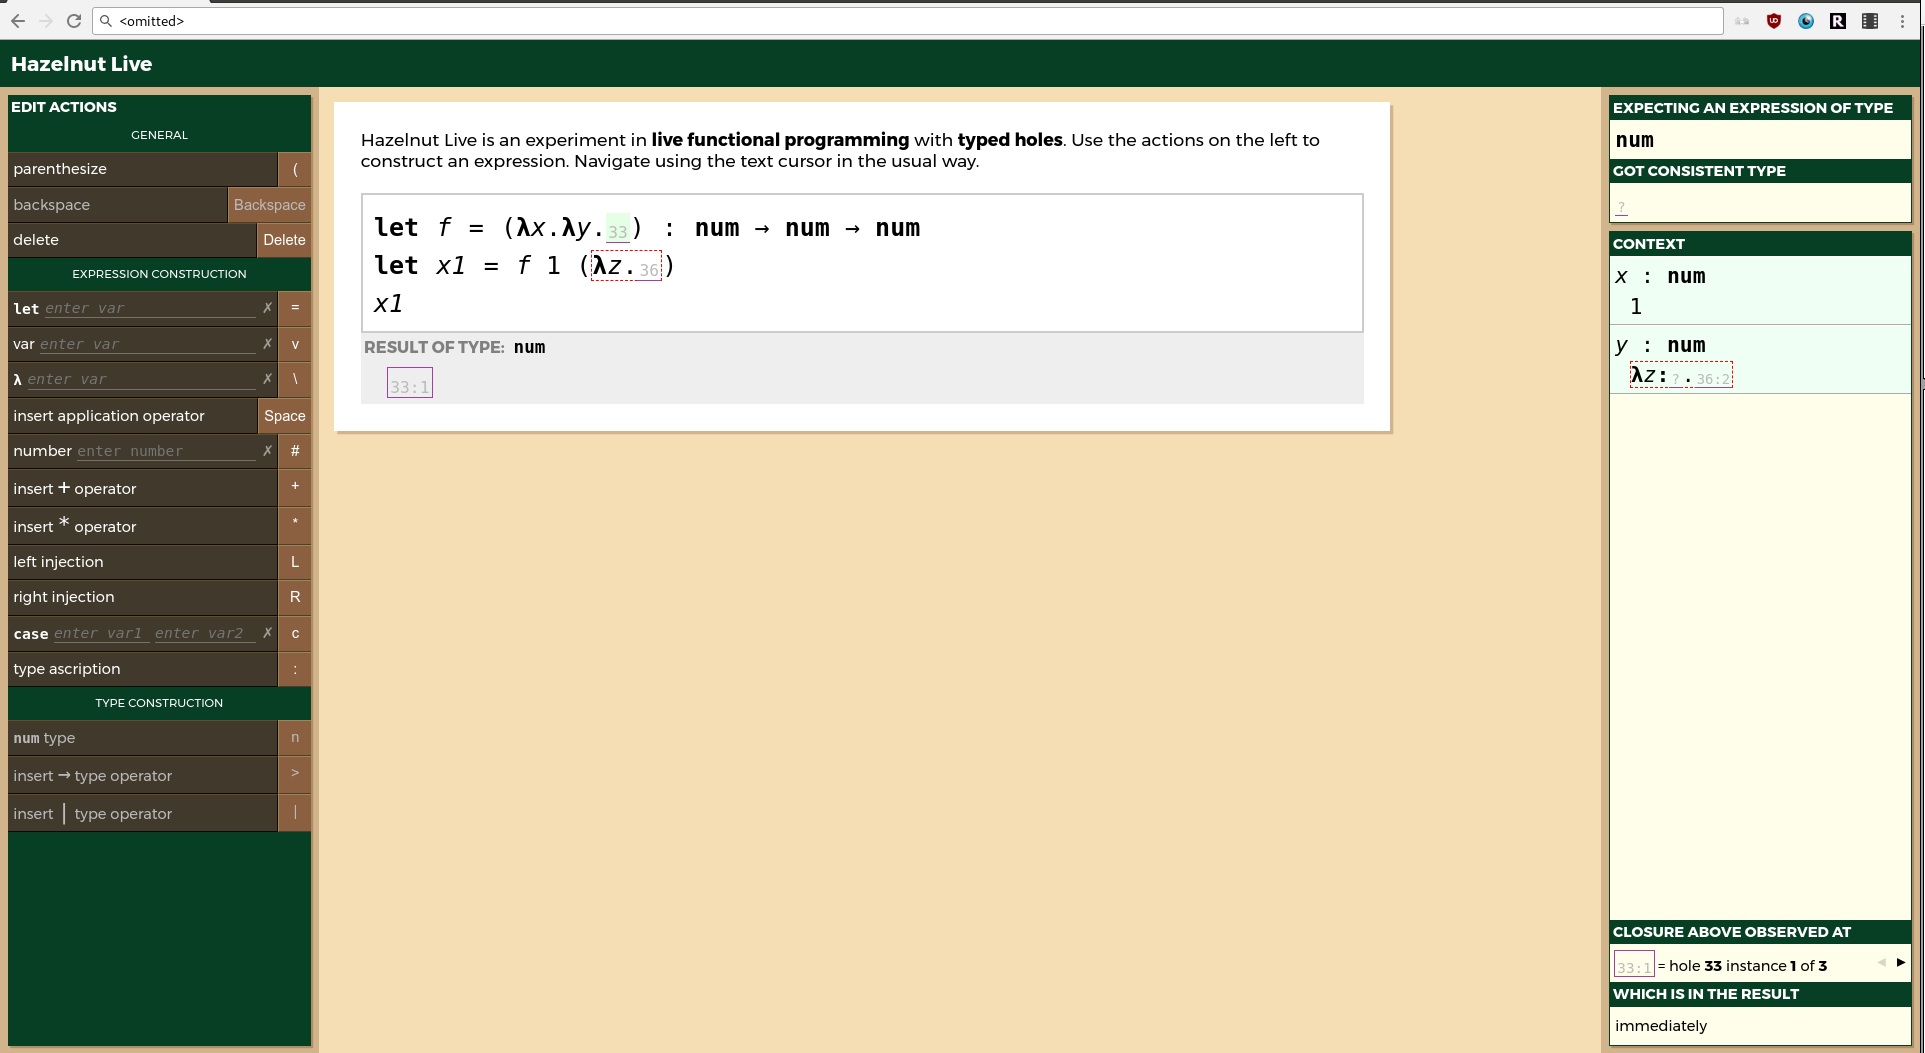
\includegraphics[width=\textwidth]{images/screenshot1.png}
\caption{This screenshot demonstrates both empty and non-empty expression holes as well as the live context inspector.}
\end{figure}

\begin{figure}[h]
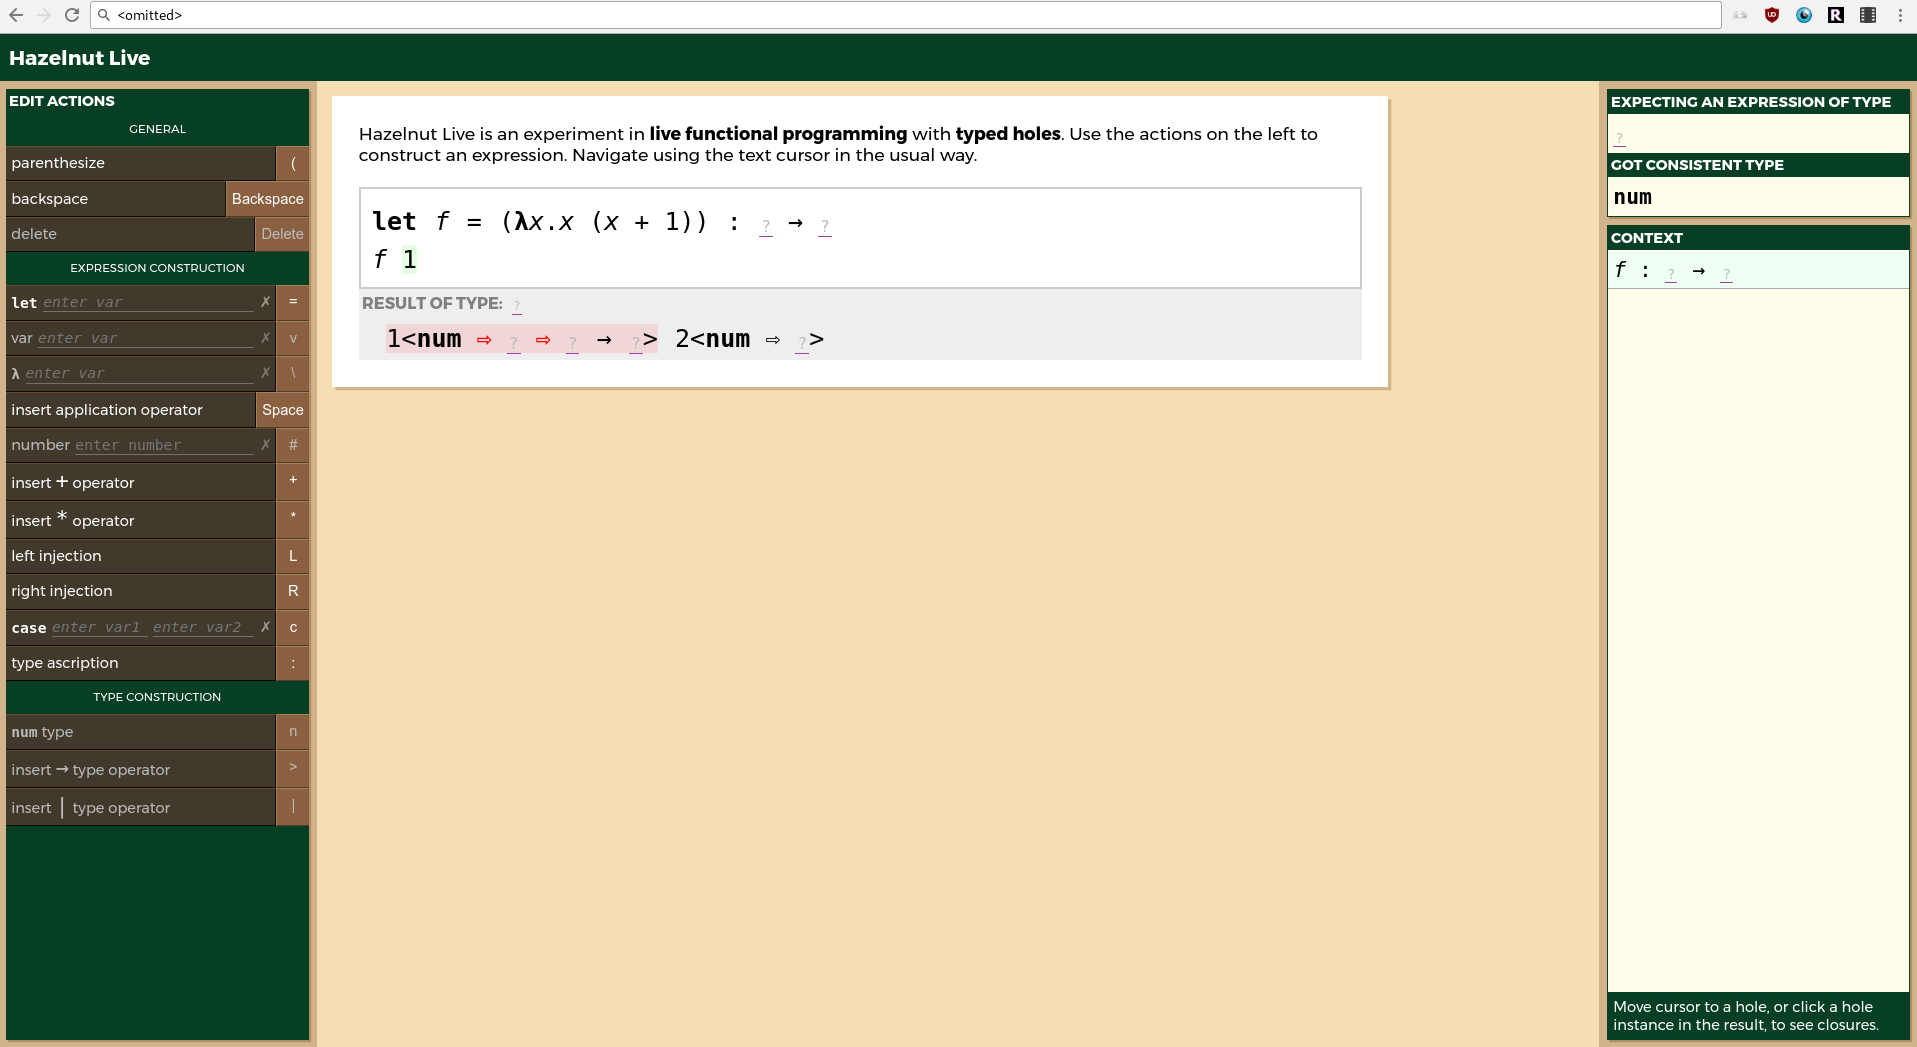
\includegraphics[width=\textwidth]{images/screenshot2.png}
\caption{This screenshot demonstrates dynamic cast failure.}
\end{figure}


\end{document}
